\documentclass[12pt,]{krantz}
\usepackage{lmodern}
\usepackage{amssymb,amsmath}
\usepackage{ifxetex,ifluatex}
\usepackage{fixltx2e} % provides \textsubscript
\ifnum 0\ifxetex 1\fi\ifluatex 1\fi=0 % if pdftex
  \usepackage[T1]{fontenc}
  \usepackage[utf8]{inputenc}
\else % if luatex or xelatex
  \ifxetex
    \usepackage{mathspec}
  \else
    \usepackage{fontspec}
  \fi
  \defaultfontfeatures{Ligatures=TeX,Scale=MatchLowercase}
    \setmonofont[Mapping=tex-ansi,Scale=0.7]{Source Code Pro}
\fi
% use upquote if available, for straight quotes in verbatim environments
\IfFileExists{upquote.sty}{\usepackage{upquote}}{}
% use microtype if available
\IfFileExists{microtype.sty}{%
\usepackage[]{microtype}
\UseMicrotypeSet[protrusion]{basicmath} % disable protrusion for tt fonts
}{}
\PassOptionsToPackage{hyphens}{url} % url is loaded by hyperref
\usepackage[unicode=true]{hyperref}
\PassOptionsToPackage{usenames,dvipsnames}{color} % color is loaded by hyperref
\hypersetup{
            pdftitle={bookdown: Escritura de libros y documentos técnicos con R Markdown},
            pdfauthor={Yihui Xie},
            colorlinks=true,
            linkcolor=Maroon,
            citecolor=Blue,
            urlcolor=Blue,
            breaklinks=true}
\urlstyle{same}  % don't use monospace font for urls
\usepackage{natbib}
\bibliographystyle{apalike}
\usepackage{color}
\usepackage{fancyvrb}
\newcommand{\VerbBar}{|}
\newcommand{\VERB}{\Verb[commandchars=\\\{\}]}
\DefineVerbatimEnvironment{Highlighting}{Verbatim}{commandchars=\\\{\}}
% Add ',fontsize=\small' for more characters per line
\usepackage{framed}
\definecolor{shadecolor}{RGB}{248,248,248}
\newenvironment{Shaded}{\begin{snugshade}}{\end{snugshade}}
\newcommand{\KeywordTok}[1]{\textcolor[rgb]{0.13,0.29,0.53}{\textbf{#1}}}
\newcommand{\DataTypeTok}[1]{\textcolor[rgb]{0.13,0.29,0.53}{#1}}
\newcommand{\DecValTok}[1]{\textcolor[rgb]{0.00,0.00,0.81}{#1}}
\newcommand{\BaseNTok}[1]{\textcolor[rgb]{0.00,0.00,0.81}{#1}}
\newcommand{\FloatTok}[1]{\textcolor[rgb]{0.00,0.00,0.81}{#1}}
\newcommand{\ConstantTok}[1]{\textcolor[rgb]{0.00,0.00,0.00}{#1}}
\newcommand{\CharTok}[1]{\textcolor[rgb]{0.31,0.60,0.02}{#1}}
\newcommand{\SpecialCharTok}[1]{\textcolor[rgb]{0.00,0.00,0.00}{#1}}
\newcommand{\StringTok}[1]{\textcolor[rgb]{0.31,0.60,0.02}{#1}}
\newcommand{\VerbatimStringTok}[1]{\textcolor[rgb]{0.31,0.60,0.02}{#1}}
\newcommand{\SpecialStringTok}[1]{\textcolor[rgb]{0.31,0.60,0.02}{#1}}
\newcommand{\ImportTok}[1]{#1}
\newcommand{\CommentTok}[1]{\textcolor[rgb]{0.56,0.35,0.01}{\textit{#1}}}
\newcommand{\DocumentationTok}[1]{\textcolor[rgb]{0.56,0.35,0.01}{\textbf{\textit{#1}}}}
\newcommand{\AnnotationTok}[1]{\textcolor[rgb]{0.56,0.35,0.01}{\textbf{\textit{#1}}}}
\newcommand{\CommentVarTok}[1]{\textcolor[rgb]{0.56,0.35,0.01}{\textbf{\textit{#1}}}}
\newcommand{\OtherTok}[1]{\textcolor[rgb]{0.56,0.35,0.01}{#1}}
\newcommand{\FunctionTok}[1]{\textcolor[rgb]{0.00,0.00,0.00}{#1}}
\newcommand{\VariableTok}[1]{\textcolor[rgb]{0.00,0.00,0.00}{#1}}
\newcommand{\ControlFlowTok}[1]{\textcolor[rgb]{0.13,0.29,0.53}{\textbf{#1}}}
\newcommand{\OperatorTok}[1]{\textcolor[rgb]{0.81,0.36,0.00}{\textbf{#1}}}
\newcommand{\BuiltInTok}[1]{#1}
\newcommand{\ExtensionTok}[1]{#1}
\newcommand{\PreprocessorTok}[1]{\textcolor[rgb]{0.56,0.35,0.01}{\textit{#1}}}
\newcommand{\AttributeTok}[1]{\textcolor[rgb]{0.77,0.63,0.00}{#1}}
\newcommand{\RegionMarkerTok}[1]{#1}
\newcommand{\InformationTok}[1]{\textcolor[rgb]{0.56,0.35,0.01}{\textbf{\textit{#1}}}}
\newcommand{\WarningTok}[1]{\textcolor[rgb]{0.56,0.35,0.01}{\textbf{\textit{#1}}}}
\newcommand{\AlertTok}[1]{\textcolor[rgb]{0.94,0.16,0.16}{#1}}
\newcommand{\ErrorTok}[1]{\textcolor[rgb]{0.64,0.00,0.00}{\textbf{#1}}}
\newcommand{\NormalTok}[1]{#1}
\usepackage{longtable,booktabs}
% Fix footnotes in tables (requires footnote package)
\IfFileExists{footnote.sty}{\usepackage{footnote}\makesavenoteenv{long table}}{}
\usepackage{graphicx,grffile}
\makeatletter
\def\maxwidth{\ifdim\Gin@nat@width>\linewidth\linewidth\else\Gin@nat@width\fi}
\def\maxheight{\ifdim\Gin@nat@height>\textheight\textheight\else\Gin@nat@height\fi}
\makeatother
% Scale images if necessary, so that they will not overflow the page
% margins by default, and it is still possible to overwrite the defaults
% using explicit options in \includegraphics[width, height, ...]{}
\setkeys{Gin}{width=\maxwidth,height=\maxheight,keepaspectratio}
\IfFileExists{parskip.sty}{%
\usepackage{parskip}
}{% else
\setlength{\parindent}{0pt}
\setlength{\parskip}{6pt plus 2pt minus 1pt}
}
\setlength{\emergencystretch}{3em}  % prevent overfull lines
\providecommand{\tightlist}{%
  \setlength{\itemsep}{0pt}\setlength{\parskip}{0pt}}
\setcounter{secnumdepth}{5}
% Redefines (sub)paragraphs to behave more like sections
\ifx\paragraph\undefined\else
\let\oldparagraph\paragraph
\renewcommand{\paragraph}[1]{\oldparagraph{#1}\mbox{}}
\fi
\ifx\subparagraph\undefined\else
\let\oldsubparagraph\subparagraph
\renewcommand{\subparagraph}[1]{\oldsubparagraph{#1}\mbox{}}
\fi

% set default figure placement to htbp
\makeatletter
\def\fps@figure{htbp}
\makeatother

\usepackage{booktabs}
\usepackage{longtable}
\usepackage[bf,singlelinecheck=off]{caption}

% \setmainfont[UprightFeatures={SmallCapsFont=AlegreyaSC-Regular}]{Alegreya}

\usepackage{framed,color}
\definecolor{shadecolor}{RGB}{248,248,248}

\renewcommand{\textfraction}{0.05}
\renewcommand{\topfraction}{0.8}
\renewcommand{\bottomfraction}{0.8}
\renewcommand{\floatpagefraction}{0.75}

\renewenvironment{quote}{\begin{VF}}{\end{VF}}
\let\oldhref\href
\renewcommand{\href}[2]{#2\footnote{\url{#1}}}

\ifxetex
  \usepackage{letltxmacro}
  \setlength{\XeTeXLinkMargin}{1pt}
  \LetLtxMacro\SavedIncludeGraphics\includegraphics
  \def\includegraphics#1#{% #1 catches optional stuff (star/opt. arg.)
    \IncludeGraphicsAux{#1}%
  }%
  \newcommand*{\IncludeGraphicsAux}[2]{%
    \XeTeXLinkBox{%
      \SavedIncludeGraphics#1{#2}%
    }%
  }%
\fi

\makeatletter
\newenvironment{kframe}{%
\medskip{}
\setlength{\fboxsep}{.8em}
 \def\at@end@of@kframe{}%
 \ifinner\ifhmode%
  \def\at@end@of@kframe{\end{minipage}}%
  \begin{minipage}{\columnwidth}%
 \fi\fi%
 \def\FrameCommand##1{\hskip\@totalleftmargin \hskip-\fboxsep
 \colorbox{shadecolor}{##1}\hskip-\fboxsep
     % There is no \\@totalrightmargin, so:
     \hskip-\linewidth \hskip-\@totalleftmargin \hskip\columnwidth}%
 \MakeFramed {\advance\hsize-\width
   \@totalleftmargin\z@ \linewidth\hsize
   \@setminipage}}%
 {\par\unskip\endMakeFramed%
 \at@end@of@kframe}
\makeatother

\renewenvironment{Shaded}{\begin{kframe}}{\end{kframe}}

\newenvironment{rmdblock}[1]
  {
  \begin{itemize}
  \renewcommand{\labelitemi}{
    \raisebox{-.7\height}[0pt][0pt]{
      {\setkeys{Gin}{width=3em,keepaspectratio}\includegraphics{images/#1}}
    }
  }
  \setlength{\fboxsep}{1em}
  \begin{kframe}
  \item
  }
  {
  \end{kframe}
  \end{itemize}
  }
\newenvironment{rmdnote}
  {\begin{rmdblock}{note}}
  {\end{rmdblock}}
\newenvironment{rmdcaution}
  {\begin{rmdblock}{caution}}
  {\end{rmdblock}}
\newenvironment{rmdimportant}
  {\begin{rmdblock}{important}}
  {\end{rmdblock}}
\newenvironment{rmdtip}
  {\begin{rmdblock}{tip}}
  {\end{rmdblock}}
\newenvironment{rmdwarning}
  {\begin{rmdblock}{warning}}
  {\end{rmdblock}}

\usepackage{makeidx}
\makeindex

\urlstyle{tt}

\title{bookdown: Escritura de libros y documentos técnicos con R Markdown}
\author{Yihui Xie}
\date{2018-01-10}

\usepackage{amsthm}
\newtheorem{theorem}{Teorema}[chapter]
\newtheorem{lemma}{Lema}[chapter]
\theoremstyle{definition}
\newtheorem{definition}{Definición}[chapter]
\newtheorem{corollary}{Corolario}[chapter]
\newtheorem{proposition}{Proposición}[chapter]
\theoremstyle{definition}
\newtheorem{example}{Ejemplo}[chapter]
\theoremstyle{definition}
\newtheorem{exercise}{Ejercicio.}[chapter]
\theoremstyle{remark}
\newtheorem*{remark}{Observación}
\newtheorem*{solution}{Solución}
\let\BeginKnitrBlock\begin \let\EndKnitrBlock\end
\begin{document}
\maketitle

\cleardoublepage\newpage\thispagestyle{empty}\null
\cleardoublepage\newpage\thispagestyle{empty}
\begin{center}
To ...
\end{center}

\setlength{\abovedisplayskip}{-5pt}
\frontmatter

{
\hypersetup{linkcolor=black}
\setcounter{tocdepth}{2}
\tableofcontents
}
\listoftables
\listoffigures
\chapter*{Prefacio}\label{prefacio}


Este breve libro presenta el paquete de R, \textbf{bookdown}, que cambia
la forma de escribir libros. Escribir un libro debe ser técnicamente
fácil, visualmente agradable a la hora de leerlo, divertido para
interactuar con él, cómodo para navegar a través de sus páginas y
sencillo si los lectores desean contribuir o dejar comentarios para
su(s) autor(es), y lo más importante, para que los autores no se
distraigan con los detalles de composición tipográfica.

El paquete \textbf{bookdown} fue construido con base en R Markdown
(\url{http://rmarkdown.rstudio.com}), y heredó la simplicidad en la
sintaxis de R Markdown (puede aprenderse lo básico en cinco minutos;
véase la sección \ref{sintaxis-de-markdown}), así como la posibilidad de
múltiples tipos de formatos de salida (PDF/HTML/Word/\ldots{}).
Asimismo, ha añadido diferentes características como la salida de
múltiples páginas HTML, numeración y referenciación cruzada a
figuras/tablas/secciones/ecuaciones, inserción de partes/apéndices, e
importación del estilo GitBook \index{GitBook}
(\url{https://www.gitbook.com}) para crear páginas de libros en un
formato elegante y atractivo en HTML. Este libro en sí es un ejemplo de
cómo se puede producir un libro de una serie de documentos R Markdown, y
tanto la versión impresa como la versión en línea puede parecer
profesional. Puede encontrar más ejemplos en \url{https://bookdown.org}.

A pesar de que el nombre del paquete contiene la palabra ``libro'',
\textbf{bookdown} no es sólo para libros. El ``libro'' puede ser
cualquier cosa que se componga de varios documentos R Markdown, como
documentación de un curso, notas de estudio, un manual de software, una
tesis de maestría/doctorado, o incluso un diario. De hecho, muchas
características de \textbf{bookdown} se aplican a documentos sencillos
de R Markdown (Sección \ref{un-documento-sencillo}).

\includegraphics{images/by-nc-sa.png}\\
La versión online de este documento está licenciada bajo la
\href{http://creativecommons.org/licenses/by-nc-sa/4.0/}{Creative
Commons Attribution-NonCommercial-ShareAlike 4.0 International License}.
You can purchase a hardcopy from
\href{https://www.crcpress.com/product/isbn/9781138700109}{Chapman \&
Hall} or Amazon.

\section*{¿Por qué leer este libro?}\label{por-que-leer-este-libro}


¿Puede escribirse un libro en un formato de origen, y generar la salida
a múltiples formatos? Tradicionalmente los libros se escriben con LaTeX
o Microsoft Word. Cualquiera de estas herramientas hará que escribir
libros sea un viaje de ida donde no se puede dar marcha atrás: si elige
LaTeX, normalmente termina sólo con un documento PDF; si se trabaja con
Word, es probable que tenga que permanecer en Word para siempre, y
también se pueden desperdiciar muchas de las características útiles y
hermosas de la salida PDF que sí genera LaTeX.

¿Puede enfocarse en escribir el contenido del libro sin tener que
preocuparse demasiado por la composición tipográfica? Parece haber una
contradicción natural entre el contenido y la apariencia, y siempre
tiene que equilibrarse el tiempo que se dedica a estos dos aspectos. Se
quiere que el libro luzca razonablemente bonito, a la vez que quiere
centrarse en su contenido. Una posibilidad es renunciar a PDF
temporalmente, y a cambio obtener una vista previa bastante bella de su
libro en páginas web HTML \index{HTML}. LaTeX \index{LaTeX} es una
excelente herramienta de composición, pero puede ahogarse fácilmente en
las numerosas órdenes de su programación y en los detalles de
composición tipográfica mientras se está trabajando en el libro. Es
difícil obtener una previsualización del libro en PDF, y, por desgracia,
algunas veces aparecen ciertas palabras que exceden el margen de la
página, algunas figuras flotan en páginas al azar, cinco o seis palabras
sueltas en el final de un capítulo llevan a una página nueva, y así
sucesivamente. Si el libro se va a imprimir, tendrá que hacer frente a
estos problemas eventualmente, y realmente no vale la pena distraerse
una y otra vez sobre estos asuntos mientras está escribiendose el libro.
El hecho de que la sintaxis de Markdown es más simple y tiene menos
funciones que LaTeX también ayuda a centrarse en el contenido del libro.
¿Realmente tiene que definirse un nuevo comando como
\texttt{\textbackslash{}myprecious\{\}} que aplica
\texttt{\textbackslash{}textbf\{\textbackslash{}textit\{\textbackslash{}textsf\{\}\}\}}
a su texto? ¿La letra ``R'' tiene que estar encerrada en
\texttt{\textbackslash{}proglang\{\}} cuando los lectores pueden
fácilmente intuir que representa el lenguaje R? No hay mucha diferencia
si todo o nada, necesita la atención del lector.

¿Pueden interactuar los lectores con ejemplos del libro cuando lo leen?
La respuesta es no, sin duda alguna, siempre y cuando el libro esté
impreso en papel, pero es posible hacerlo si su libro tiene una versión
HTML que contenga ejemplos interactivos, como las aplicaciones Shiny
(\url{https://shiny.rstudio.com}) o los HTML widgets
(\url{https://htmlwidgets.org}). Por ejemplo, los lectores pueden saber
de inmediato qué pasa si cambian algunos parámetros en un modelo
estadístico.

¿Puede obtener retroalimentación e incluso contribuciones de los
lectores a medida que se escribe el libro? Tradicionalmente, el editor
puede encontrar un pequeño número de revisores anónimos para corregir su
libro. Los revisores suelen ser útiles, pero es posible que aún así se
pierda el aporte de los lectores más representativos. Es demasiado tarde
después de que se imprimió la primera edición, y el lector tiene que
esperar unos años antes que la segunda edición esté lista. Hay algunas
plataformas web que hacen que sea fácil para las personas proporcionar
retroalimentación y contribución a sus proyectos, y GitHub
(\url{https://github.com}) es un ejemplo prominente. Si alguien
encuentra un error tipográfico en su libro, puede simplemente corregirlo
en línea y enviarle el cambio para su aprobación. Es una cuestión de
hacer clic en un botón para fusionar el cambio, sin hacer preguntas o
correos electrónicos de ida y vuelta. Para poder utilizar estas
plataformas, es necesario aprender los conceptos básicos de herramientas
de control de versiones como GIT, y los archivos de origen del libro
deben estar en texto plano.

La combinación de R (\url{https://www.r-project.org}), Markdown, y
Pandoc (\url{http://pandoc.org}) hace que sea posible pasar de un
formato de fuente simple (R Markdown) a múltiples formatos de salida
posibles (PDF, HTML, EPUB y Word, etc). El paquete \textbf{bookdown}
está basado en R Markdown, y proporciona formatos de salida para libros
y artículos de formato largo, incluyendo el formato GitBook, que es un
formato de salida HTML de varias páginas con una interfaz de usuario
útil y bonita. Es mucho más fácil componer en HTML que en LaTeX, por lo
que siempre se puede obtener una previsualización de su libro en HTML, y
el trabajo sobre el PDF del contenido está casi hecho. Los ejemplos
interactivos se pueden incorporar fácilmente en HTML, lo que puede hacer
al libro más atractivo y útil. R Markdown es un formato de texto plano,
lo que también puede brindar beneficios al control de versiones, como
colaborar en GitHub. También se ha tratado de poner algunas de las
características importantes de LaTeX a HTML y otros formatos de salida,
como enumeración de figuras/tablas y referenciación cruzada.

En resumen, únicamente prepare un par de capítulos de un libro en R
Markdown, y \textbf{bookdown} puede ayudarle a convertirlos en un
hermoso libro.

\section*{Estructura del libro}\label{estructura-del-libro}


Los capítulos \ref{introduccion} y \ref{componentes} introducen el uso
básico y la sintaxis, lo cual debería ser suficiente para que la mayoría
de los lectores empiecen a escribir un libro. Los capítulos
\ref{formatos-de-salida} y \ref{personalizacion} son para aquellos que
quieren afinar la apariencia de sus libros. Pueden parecer muy técnicos
si no se está familiarizados con HTML/CSS y LaTeX. No es necesario leer
estos dos capítulos con mucho cuidado la primera vez. Puede aprender lo
que posiblemente puede cambiarse, y volver después para saber cómo
hacerlo. Para el capítulo \ref{edicion}, los detalles técnicos no son
importantes a menos que no utilice el RStudio IDE (Sección
\ref{ide-rstudio}). Del mismo modo, puede sentirse abrumado por los
comandos presentados en el capítulo \ref{publicacion} para publicar su
libro, pero nuevamente, hemos tratado de facilitar la publicación de su
libro en línea a través de la IDE de RStudio. Los comandos y funciones
personalizadas son sólo para aquellos que deciden no usar el servicio de
RStudio o quieren entender los detalles técnicos.

Para resumir, este libro es una referencia completa del paquete
\textbf{bookdown}. Puede seguir la regla 80/20 al leerla. Algunas
secciones están allí para el bien de la integridad, y no todas las
secciones son igualmente útiles al libro particular que usted piensa
escribir.

\section*{Información acerca del software y
convenciones}\label{informacion-acerca-del-software-y-convenciones}
\addcontentsline{toc}{section}{Información acerca del software y
convenciones}

Este libro es principalmente sobre el paquete \textbf{bookdown} de R,
por lo que necesita instalar al menos R y el paquete \textbf{bookdown}.
Sin embargo, su libro no tiene que estar relacionado en absoluto con el
lenguaje R. Se pueden usar otros lenguajes de computación (C++, SQL,
Python, etc.; véase el Apéndice \ref{uso-de-software}), e incluso puede
ser totalmente irrelevante para la computación (por ejemplo, puede
escribir una novela, o una colección de poemas). Las herramientas de
software necesarias para construir un libro se introducen en el Apéndice
\ref{herramientas-de-software}.

La información de la sesión de R al compilar este libro es la siguiente:

\begin{Shaded}
\begin{Highlighting}[]
\KeywordTok{sessionInfo}\NormalTok{()}
\end{Highlighting}
\end{Shaded}

\begin{verbatim}
## R version 3.4.3 (2017-11-30)
## Platform: x86_64-apple-darwin15.6.0 (64-bit)
## Running under: macOS High Sierra 10.13.2
## 
## Matrix products: default
## BLAS: /Library/Frameworks/R.framework/Versions/3.4/Resources/lib/libRblas.0.dylib
## LAPACK: /Library/Frameworks/R.framework/Versions/3.4/Resources/lib/libRlapack.dylib
## 
## locale:
## [1] en_US.UTF-8/en_US.UTF-8/en_US.UTF-8/C/en_US.UTF-8/en_US.UTF-8
## 
## attached base packages:
## [1] stats     graphics  grDevices utils     datasets 
## [6] base     
## 
## other attached packages:
## [1] gdtools_0.1.6
## 
## loaded via a namespace (and not attached):
## [1] knitr_1.18      tools_3.4.3     miniUI_0.1.1   
## [4] htmltools_0.3.6 bookdown_0.5    shiny_1.0.5    
## [7] rmarkdown_1.8
\end{verbatim}

No se añaden instrucciones (\texttt{\textgreater{}} y \texttt{+}) al
código fuente en R en este libro, y, por defecto, se comenta la salida
de texto mediante dos numerales \texttt{\#\#}, como se pudo advertir
anteriormente en la información de sesión de R . Esto es para comodidad
del lector a la hora que desee copiar y ejecutar el código (el texto
resultante se ignorará ya que se encuentra comentado). Los nombres de
paquetes están en negrita (por ejemplo, \textbf{rmarkdown}), y el código
en línea y los nombres de archivos se formatean en una fuente de máquina
de escribir (por ejemplo,
\texttt{knitr::knit(\textquotesingle{}foo.Rmd\textquotesingle{})}). Los
nombres de funciones son seguidas por paréntesis (por ejemplo,
\texttt{bookdown::render\_book()}). El operador doble dos puntos
(\texttt{::}) significa acceder a un objeto desde un paquete.

\section*{Agradecimientos}\label{agradecimientos}


En primer lugar me gustaría dar las gracias a mi empleador, RStudio, por
darme la oportunidad de trabajar en este emocionante proyecto. Tenía la
esperanza de trabajar en él cuando vi por primera vez el proyecto
GitBook en 2013, ya que de inmediato me di cuenta que era un estilo
hermoso de libro y había mucha más potencia que podríamos agregarle, a
juzgar por mi experiencia de escribir el libro sobre \textbf{knitr}
\citep{xie2015} y la lectura de otros libros. R Markdown se convirtió en
un proyecto maduro dos años después, y por suerte, \textbf{bookdown} se
convirtió en mi trabajo oficial a finales de 2015. No hay muchas cosas
en el mundo mejores que el hecho de que su trabajo pase a ser su afición
(o viceversa). Estoy totalmente complacido de jugar un poco con
bibliotecas de JavaScript, paquetes de LaTeX, y un sinfín de expresiones
regulares en R. Honestamente también debo agradecer a StackOverflow
(\url{http://stackoverflow.com}), y creo que todos ustedes saben
\href{http://bit.ly/2cWbiAp}{lo que quiero decir}, si alguna vez han
escrito algún código de programa.

Este proyecto es, sin duda, no solo el esfuerzo de una sola persona.
Varios colegas en RStudio me han ayudado a lo largo del camino. Hadley
Wickham proporcionó una enorme cantidad de información durante el
desarrollo de \textbf{bookdown}, mientras trabajaba en su libro \emph{R
for Data Science} con Garrett Grolemund. JJ Allaire y Jonathan McPherson
proporcionaron una gran cantidad de ayuda técnica directamente al
paquete, así como apoyo en el IDE RStudio. Jeff Allen, Chaita Chaudhari,
y el equipo de RStudio Connect han mantenido el sitio web
\url{https://bookdown.org}. Robby Shaver diseñó una imagen de portada
bonita para este libro. Tareef Kawaf hizo todo lo posible para ayudarme
a crecer como un ingeniero de software profesional. Es una bendición
trabajar en esta empresa con personas entusiastas e inteligentes.
Recuerdo que una vez le dije a Jonathan ``Hey, me encontré con un
problema en el almacenamiento en caché de HTML widgets y finalmente me
di cuenta de una posible solución'', y Jonathan agarró su cerveza, ``yo
ya lo resolví'' ``Oh, bien, muy bien.''

También he recibido un montón de comentarios de los autores de libros
fuera de RStudio, incluyendo Jan de Leeuw, Jenny Bryan, Dean Attali,
Rafael Irizarry, Michael Love, Roger Peng, Andrew Clark, etc. Algunos
usuarios también contribuyeron con código para el proyecto y ayudaron a
revisar el libro. Aquí está una lista de todos los contribuyentes:
\url{https://github.com/rstudio/bookdown/graphs/contributors}. Se siente
bien cuando uno inventa una herramienta y se da cuenta que también es el
beneficiario de su propia herramienta. Como alguien que ama el modelo de
solicitud de extracción de GitHub, deseaba que los lectores no tuvieran
que enviarme un correo electrónico para mencionar que había un error
tipográfico o un error evidente en mi libro, sino que sólo pudiera
arreglarse a través de una solicitud de extracción. Esto fue posible en
\textbf{bookdown}. Se puede ver el número de solicitudes de extracción
de los errores tipográficos que he fusionado:
\url{https://github.com/rstudio/bookdown/pulls} Es bueno tener tantos
correctores ortográficos humanos. No es que no sepa cómo usar un
verdadero corrector ortográfico, pero no quiero hacer esto antes de que
el libro esté terminado, y el malévolo Yihui también quiere dejar
algunas tareas sencillas para los lectores e involucrarlos en la mejora
del libro.

Callum Webb amablemente diseñó un lindo sticker hexagonal para
\textbf{bookdown}.

El paquete \textbf{bookdown} no sería posible sin un par de paquetes de
software de código abierto. En particular, Pandoc, GitBook, jQuery, y
los paquetes de R dependientes, por no hablar de R en sí. Doy las
gracias a los desarrolladores de estos paquetes.

Me mudé a Omaha, Nebraska en 2015, y disfruté de un año en apartamentos
Steeplechase, donde viví con comodidad para desarrollar el paquete
\textbf{bookdown}, gracias al personal del condominio que fue muy amable
y servicial. Luego me encontré con un agente inmobiliario profesional y
muy listo, Kevin Schaben, que encontró una casa fabulosa para nosotros
en un período de tiempo sorprendentemente corto, y terminé este libro en
nuestra nueva casa.

John Kimmel, el editor de Chapman \& Hall/CRC, me ayudó a publicar mi
primer libro. Es un placer trabajar con él de nuevo. Él generosamente
accedió a que me quedara con la versión en línea de este libro de forma
gratuita, por lo que puede seguirlo para actualizar después de que se
imprima y publique (es decir, usted no tiene que esperar años para la
segunda edición para corregir errores e introducir nuevas
caracteristicas). Me gustaría poder ser lo más abierto de mente posible
como él cuando tenga su edad. Shashi Kumar resolvió algunos de mis
problemas técnicos con la clase del editor de LaTeX
(\texttt{krantz.cls}) cuando yo estaba tratando de integrarlo con
\textbf{bookdown}. También aprecio los comentarios muy útiles de los
revisores Jan de Leeuw, Karl Broma n, Brooke Anderson, Michael Grayling,
Daniel Kaplan y Max Kuhn.

Por último quiero agradecer a mi familia, en especial, a mi esposa e
hijo, por su apoyo. Él, de un año de edad, ha descubierto que el monitor
se enciende cuando toca el teclado, así que en ocasiones simplemente
gatea en mi oficina y presiona al azar el teclado. No estoy seguro de si
esto cuenta como su contribución al libro \ldots{} @)!\%)Y@*

\BeginKnitrBlock{flushright}
Yihui Xie\\
Elkhorn, Nebraska
\EndKnitrBlock{flushright}

\chapter*{Acerca del Autor}\label{acerca-del-autor}


Yihui Xie (\url{http://yihui.name}) es ingeniero de software en RStudio
(\url{http://www.rstudio.com}). Obtuvo su PhD del Departmento de
Estadística de la Iowa State University. Se interesa por los gráficos
estadísticos interactivos y la computación estadística. Como un usuario
activo de R, es autor de varios paquetes, tales como \textbf{knitr},
\textbf{bookdown}, \textbf{animation}, \textbf{DT}, \textbf{tufte},
\textbf{formatR}, \textbf{fun}, \textbf{mime}, \textbf{highr},
\textbf{servr}, y \textbf{Rd2roxygen}, entre los cuales el paquete
\textbf{animation} ganó el premio de Software Estadístico John M.
Chambers (ASA) en 2009. También es coautor de otros pocos paquetes de R,
incluyendo \textbf{shiny}, \textbf{rmarkdown}, y \textbf{leaflet}.

En 2006, fundó el ``Capital of Statistics'' (\url{http://cos.name}), que
ha crecido hasta convertirse en una gran comunidad de estadísticos en
China. Inició la conferencia china de R en 2008, y ha estado involucrado
en la organización de conferencias sobre R en China desde entonces.
Durante su estadía en el PhD en la Iowa State University, ganó el premio
de Computación Estadística Vince Sposito (2011) y el premio Snedecor
(2012) en el Departmento de Estadística.

Ocasionalmente despotrica en Twitter
(\url{https://twitter.com/xieyihui}), y la mayor parte del tiempo se
encuentra en GitHub (\url{https://github.com/yihui}).

Adora la comida picante tanto como la literatura china clásica.

\mainmatter

\chapter{Introducción}\label{introduccion}

Este libro es una guía para la escritura de libros con R Markdown
\citep{R-rmarkdown} y con el paquete \textbf{bookdown} de R
\citep{R-bookdown}. Se enfoca en las características específicas de la
escritura de libros, artículos o reportes de gran extensión . Algunas de
estas características son:

\begin{itemize}
\item
  Cómo se componen figuras y tablas y se hacen referencias cruzadas
  hacia ellas;
\item
  Cómo generar múltiples formatos de salida tales como HTML, PDF y
  e-books para un sólo libro;
\item
  Como personalizar las plantillas de los libros y elementos de
  diferentes estilos en un libro;
\item
  El soporte de editor (en particular, el IDE RStudio);
\item
  Cómo publicar un libro;
\end{itemize}

No es una completa introducción a R Markdown o al paquete \textbf{knitr}
\citep{R-knitr}, sobre el cual se construyó \textbf{bookdown}. Para
obtener más información sobre R Markdown, consulte la documentación en
línea \url{http://rmarkdown.rstudio.com}. Para \textbf{knitr}, consulte
\citet{xie2015}. No hay que ser un experto en el lenguaje R
\citep{R-base} para leer este libro, pero se espera que se tengan
conocimientos básicos sobre R Markdown y \textbf{knitr}. Para los
principiantes, puede empezar a trabajar con los Cheatsheets en
\url{https://www.rstudio.com/resources/cheatsheets/}. El apéndice de
este libro contiene breves introducciones a esos paquetes de software.
Para poder personalizar las plantillas de libros y temas, debe estar
familiarizado con LaTeX, HTML y CSS.

\section{Motivación}\label{motivacion}

Markdown es un maravilloso lenguaje para escribir documentos
relativamente simples que contengan elementos como secciones, párrafos,
listas, vínculos e imágenes, etc. Pandoc \url{http://pandoc.org} ha
extendido enormemente la
\href{http://daringfireball.net/projects/markdown/}{sintaxis original de
Markdown} y ha añadido unas pequeñas nuevas características tales como
notas al pie de página, citas y tablas. Lo más importante que hace
Pandoc es hacer posible la generación de documentos en una amplia
variedad de formatos desde Markdown, incluyendo HTML, LaTeX/PDF, MSWord
y Slides.

Existen unas pocas características que Pandoc aún no permite hacer si lo
que se desea es escribir un documento como un libro relativamente
complicado, tales como numerar automáticamente las figuras y tablas en
la salida de documentos HTML, referencias cruzadas de figuras y tablas y
un control óptimo de la apariencia de figuras (e.g.~actualmente es
imposible especificar la alineación de imágenes usando la sintaxis de
Markdown). Estos son algunos de los problemas que se han intentado
resolver con la librería \textbf{bookdown}.

Bajo la restricción de que queremos producir el libro en varios formatos
de salida, es casi imposible cubrir todas las posibles características
específicas de estos formatos. Por ejemplo, puede ser difícil recrear un
determinado ambiente complicado en LaTeX en la salida HTML utilizando la
sintaxis de R Markdown. El objetivo principal no es reemplazar
\emph{todo} con Markdown, sino cubrir las funcionalidades más comunes
que se requieren para escribir un documento relativamente complicado, y
hacer la sintaxis de dichas funcionalidades consistentes a través de
todos los formatos de salida, por lo que sólo necesita aprenderse una
cosa y ésta funciona bien para todos los formatos de
salida.\index{Markdown}\index{LaTeX}

Otro de los objetivos de este proyecto es hacer que sea fácil producir
libros que parezcan visualmente agradables. Algunos buenos ejemplos
existentes incluyen Gitbook \url{https://www.gitbook.com}, Tufte CSS
\url{http://edwardtufte.github.io/tufte-css/}, y Tufte-LaTeX
\url{https://tufte-latex.github.io/tufte-latex/}. Se espera integrar
estos temas y estilos en \textbf{bookdown}, por lo que los autores no
tienen que sumergirse en los detalles sobre cómo utilizar una cierta
clase de plantilla LaTeX o cómo configurar CSS para la salida HTML.

\section{Comenzando}\label{comenzando}

El camino más fácil para que los principiantes comiencen con la
escritura de un libro con R Markdown y \textbf{bookdown} es a través de
la demostración \texttt{bookdown-demo} en GitHub:

\begin{enumerate}
\def\labelenumi{\arabic{enumi}.}
\item
  Descargue el repositorio de GitHub
  \url{https://github.com/rstudio/bookdown-demo} como un {[}archivo
  Zip{]} y luego descomprímalo localmente;
\item
  Instale el IDE RStudio. Observe que necesita una versión superior a la
  1.0.0. Por favor
  \href{https://www.rstudio.com/products/rstudio/download/preview/}{descargue
  la última versión} si su versión de RStudio es menor a la 1.0.0);
\item
  Instale el paquete de R \textbf{bookdown}:

\begin{Shaded}
\begin{Highlighting}[]
\CommentTok{# version estable en el CRAN}
\KeywordTok{install.packages}\NormalTok{(}\StringTok{'bookdown'}\NormalTok{)}
\CommentTok{# o la versión de desarrollo en GitHub}
\CommentTok{# devtools::install_github('rstudio/bookdown')}
\end{Highlighting}
\end{Shaded}
\item
  Abra el repositorio \texttt{bookdown-demo} que descargó en RStudio
  haciendo click en \texttt{bookdown-demo.Rproj}.
\item
  Abra el archivo de R Markdown \texttt{index.Rmd} y haga clic en el
  botón \texttt{Build\ Book} en la pestaña \texttt{Build} de RStudio;
\end{enumerate}

Ahora debería ver la página de índice de ese libro de demostración en el
visor de RStudio. Puede agregar o cambiar los archivos de R Markdown,
volver a \texttt{index.Rmd}, y pulsar el botón \texttt{Knit} de nuevo
para obtener una vista previa del libro. Si prefiere no utilizar
RStudio, también puede compilar el libro a través de línea de comandos.
Consulte la siguiente sección para más detalles.

Aunque se ve un buen número de archivos en el ejemplo
\texttt{bookdown-demo}, la mayoría de ellos no son esenciales para un
libro. Si se siente abrumado por el número de archivos, puede utilizar
este mínimo ejemplo, en lugar del otro, que es esencialmente un archivo
\texttt{index.Rmd}: \url{https://github.com/yihui/bookdown-minimal} El
ejemplo \texttt{bookdown-demo} contiene algunas configuraciones
avanzadas que es posible que desee aprender más adelante, como la forma
de personalizar el preámbulo de LaTeX, modificar el CSS, y construir el
libro en GitHub, etc.

\section{Uso}\label{uso}

Normalmente, un libro contiene varios capítulos, y un capítulo está
contenido dentro de un archivo de R Markdown, con la extensión de
archivo \texttt{.Rmd}. Cada archivo de R Markdown debe comenzar
inmediatamente con el título del capítulo usando el encabezado de primer
nivel, por ejemplo, \texttt{\#\ Título\ del\ Capítulo}. Todos los
archivos R Markdown deben ser codificados en UTF-8. Aquí hay un ejemplo
(las viñetas son los nombres de archivo, seguidos por el contenido del
archivo):

\begin{itemize}
\item
  index.Rmd

\begin{Shaded}
\begin{Highlighting}[]
\FunctionTok{# Prefacio \{-\}}

\NormalTok{En este libro presentamos un método interesante.}
\end{Highlighting}
\end{Shaded}
\item
  01-intro.Rmd

\begin{Shaded}
\begin{Highlighting}[]
\FunctionTok{# Introducción}

\NormalTok{Este capítulo es un panorama de los métodos con que proponemos resolver un  **problema importante**.}
\end{Highlighting}
\end{Shaded}
\item
  02-literatura.Rmd

\begin{Shaded}
\begin{Highlighting}[]
\FunctionTok{# Literatura}

\NormalTok{Aquí hay una revisión de los métodos existentes.}
\end{Highlighting}
\end{Shaded}
\item
  03-metodos.Rmd

\begin{Shaded}
\begin{Highlighting}[]
\FunctionTok{# Métodos}

\NormalTok{Describimos nuestros métodos en este capítulo.}
\end{Highlighting}
\end{Shaded}
\item
  04-aplicacion.Rmd

\begin{Shaded}
\begin{Highlighting}[]
\FunctionTok{# Aplicaciones}

\NormalTok{Algunos aplicaciones _significativas_ se demuestran}
\NormalTok{en este capítulo.}

\FunctionTok{## Ejemplo uno}

\FunctionTok{## Ejemplo dos}
\end{Highlighting}
\end{Shaded}
\item
  05-resumen.Rmd

\begin{Shaded}
\begin{Highlighting}[]
\FunctionTok{# Palabras finales}

\NormalTok{Hemos finalizado un bello libro.}
\end{Highlighting}
\end{Shaded}
\end{itemize}

De forma predeterminada, \textbf{bookdown} fusiona todos los archivos
Rmd por el orden de los nombres de archivo, por ejemplo,
\texttt{01-intro.Rmd} aparecerá antes de \texttt{02-literatura.Rmd}. Los
nombres de archivo que comiencen con un guión bajo \texttt{\_} se
omiten. Si existe un archivo Rmd llamado \texttt{index.Rmd}, siempre va
a ser tratado como el primer archivo cuando se fusionen todos los
archivos Rmd. La razón de este tratamiento especial es que el archivo
HTML \texttt{index.html} se genera a partir de\texttt{index.Rmd}. Este
\texttt{index.html} suele ser el archivo de índice por defecto cuando se
ve una página web, por ejemplo, usted está viendo
\url{http://yihui.name/index.html} cuando se abre
\url{http://yihui.name/}.

Puede anular el comportamiento anterior mediante la inclusión de un
archivo de configuración llamado \texttt{\_bookdown.yml} en el
directorio del libro. Este es un archivo YAML
(\url{https://en.wikipedia.org/wiki/YAML}), y los usuarios de R Markdown
deben estar familiarizados con este formato, ya que también se utiliza
para escribir los metadatos al comienzo de los documentos R Markdown
(puede aprender más acerca de YAML en la Sección \ref{r-markdown}).
Puede utilizar un campo llamado \texttt{rmd\_files} para definir su
propia lista y el orden de los archivos Rmd para el libro. Por ejemplo,

\begin{Shaded}
\begin{Highlighting}[]
\FunctionTok{rmd_files:}\AttributeTok{ }\KeywordTok{[}\StringTok{"index.Rmd"}\KeywordTok{,} \StringTok{"abstract.Rmd"}\KeywordTok{,} \StringTok{"intro.Rmd"}\KeywordTok{]}
\end{Highlighting}
\end{Shaded}

En este caso, \textbf{bookdown} sólo tiene que utilizar lo que se ha
definido en este campo YAML sin tratamientos especiales de
\texttt{index.Rmd} o guiones bajos. Si desea salidas HTML y LaTeX/PDF
del libro, y usar diferentes archivos Rmd para la salida HTML y LaTeX,
puede especificar estos archivos para los dos formatos de salida por
separado, por ejemplo,

\begin{Shaded}
\begin{Highlighting}[]
\FunctionTok{rmd_files:}
  \FunctionTok{html:}\AttributeTok{ }\KeywordTok{[}\StringTok{"index.Rmd"}\KeywordTok{,} \StringTok{"abstract.Rmd"}\KeywordTok{,} \StringTok{"intro.Rmd"}\KeywordTok{]}
  \FunctionTok{latex:}\AttributeTok{ }\KeywordTok{[}\StringTok{"abstract.Rmd"}\KeywordTok{,} \StringTok{"intro.Rmd"}\KeywordTok{]}
\end{Highlighting}
\end{Shaded}

A pesar de que hemos estado hablando acerca de los archivos de R
Markdown, los archivos de capítulos en realidad no tienen que ser R
Markdown. Pueden ser archivos sin formato Markdown ( \texttt{.md}), y no
tienen que contener trozos de código R (en adelante \emph{chunks}) en
absoluto. ¡Por supuesto que puede utilizar \textbf{bookdown} para
componer novelas o poemas!

Por el momento, los principales formatos de salida que se pueden
utilizar incluyen
\texttt{bookdown::pdf\_book},\texttt{bookdown::gitbook},
\texttt{bookdown::html\_book}, y \texttt{bookdown::epub\_book}. Hay una
función \texttt{bookdown::render\_book()}
\index{bookdown::render\_book()} similar a \texttt{rmarkdown::render()},
pero fue diseñada para hacer \emph{múltiples} documentos Rmd en un libro
utilizando las funciones de formato de salida. Es posible que se quiera
llamar a esta función desde la línea de comandos directamente, o hacer
clic en los botones correspondientes en el IDE RStudio. Estos son
algunos ejemplos de línea de comandos:

\begin{Shaded}
\begin{Highlighting}[]
\NormalTok{bookdown}\OperatorTok{::}\KeywordTok{render_book}\NormalTok{(}\StringTok{'foo.Rmd'}\NormalTok{, }\StringTok{'bookdown::gitbook'}\NormalTok{)}
\NormalTok{bookdown}\OperatorTok{::}\KeywordTok{render_book}\NormalTok{(}\StringTok{'foo.Rmd'}\NormalTok{, }\StringTok{'bookdown::pdf_book'}\NormalTok{)}
\NormalTok{bookdown}\OperatorTok{::}\KeywordTok{render_book}\NormalTok{(}\StringTok{'foo.Rmd'}\NormalTok{, bookdown}\OperatorTok{::}\KeywordTok{gitbook}\NormalTok{(}\DataTypeTok{lib_dir =} \StringTok{'libs'}\NormalTok{))}
\NormalTok{bookdown}\OperatorTok{::}\KeywordTok{render_book}\NormalTok{(}\StringTok{'foo.Rmd'}\NormalTok{, bookdown}\OperatorTok{::}\KeywordTok{pdf_book}\NormalTok{(}\DataTypeTok{keep_tex =} \OtherTok{TRUE}\NormalTok{))}
\end{Highlighting}
\end{Shaded}

Para utilizar las funciones \texttt{render\_book} y el formato de salida
en el IDE RStudio, se puede definir un campo YAML llamado \texttt{site}
que toma el valor \texttt{bookdown::bookdown\_site} \footnote{Esta
  función llama a \texttt{bookdown::render\_book()}.}, y las funciones
de formato de salida se pueden utilizar en el campo \texttt{output}, por
ejemplo,

\begin{Shaded}
\begin{Highlighting}[]
\OtherTok{---}
\FunctionTok{site:}\AttributeTok{ }\StringTok{"bookdown::bookdown_site"}
\FunctionTok{output:}
  \FunctionTok{bookdown:}\AttributeTok{:gitbook:}
    \FunctionTok{lib_dir:}\AttributeTok{ }\StringTok{"book_assets"}
  \FunctionTok{bookdown:}\AttributeTok{:pdf_book:}
    \FunctionTok{keep_tex:}\AttributeTok{ yes}
\OtherTok{---}
\end{Highlighting}
\end{Shaded}

A continuación, puede hacer clic en el botón \texttt{Build\ Book} en el
panel \texttt{Build} en RStudio para compilar los archivos Rmd en un
libro, o haga clic en el botón \texttt{Knit} en la barra de herramientas
para obtener una vista previa del capítulo actual.

Más opciones de configuración \textbf{bookdown} en
\texttt{\_bookdown.yml} se explican en la sección \ref{configuracion}.
Además de estas configuraciones, también puede especificar otras
relacionadas con Pandoc en los metadatos YAML del primer archivo Rmd del
libro, como el título, autor y fecha del libro, etc. Por ejemplo:

\begin{Shaded}
\begin{Highlighting}[]
\OtherTok{--- }
\FunctionTok{title:}\AttributeTok{ }\StringTok{"Creando un libro con R Markdown"}
\FunctionTok{author:}\AttributeTok{ }\StringTok{"Yihui Xie"}
\FunctionTok{date:}\AttributeTok{ }\StringTok{"`r Sys.Date()`"}
\FunctionTok{site:}\AttributeTok{ }\StringTok{"bookdown::bookdown_site"}
\FunctionTok{output:}
  \FunctionTok{bookdown:}\AttributeTok{:gitbook: default}
\FunctionTok{documentclass:}\AttributeTok{ book}
\FunctionTok{bibliography:}\AttributeTok{ }\KeywordTok{[}\StringTok{"book.bib"}\KeywordTok{,} \StringTok{"packages.bib"}\KeywordTok{]}
\FunctionTok{biblio-style:}\AttributeTok{ apalike}
\FunctionTok{link-citations:}\AttributeTok{ yes}
\OtherTok{---}
\end{Highlighting}
\end{Shaded}

\section{Dos enfoques de representación}\label{new-session}

Fusionar todos los capítulos en un archivo Rmd y compilarlo es una
manera de hacer el libro en \textbf{bookdown}. Actualmente, existe otra
forma: es posible compilar cada capítulo en una sesión de R
\emph{separada}, y \textbf{bookdown} combinará los Markdown de todos los
capítulos para hacer el libro. A estos dos enfoques se les llama ``Merge
and knit'' (MK) y ``knit and Merge'' (KM), respectivamente. Las
diferencias entre ellos parecen sutiles, pero pueden ser bastante
importantes dependiendo de sus casos de uso.

\begin{itemize}
\tightlist
\item
  La diferencia más significativa es que el MK corre \emph{todos} los
  trozos de código de todos los capítulos en la misma sesión de R,
  mientras que K-M utiliza sesiones de R separadas para los distintos
  capítulos. Para M-K, el estado de la sesión de R de los capítulos
  anteriores se lleva a capítulos posteriores (por ejemplo, los objetos
  creados en los capítulos anteriores están disponibles para los
  capítulos siguientes, a menos que se les elimine deliberadamente);
  para K-M, todos los capítulos están aislados unos de otros\footnote{Obviamente,
    nadie puede dejar de escribir algunos archivos en un capítulo, y
    leerlos en otro capítulo. Es difícil aislar este tipo de efectos
    colaterales}. Si desea que cada capítulo se compile desde un estado
  limpio, utilice el enfoque K-M. Puede ser muy complicado y difícil
  restaurar una sesión de R corriendo a un estado completamente limpio
  si se utiliza el enfoque de M-K. Por ejemplo, incluso si desea
  desvincular/descargar paquetes previamente cargados en un capítulo
  previo, R no va a limpiar los métodos S3 registrados por los paquetes.
\item
  Debido a que \textbf{knitr} no permite etiquetas de chunk duplicadas
  en un documento de origen, debe asegurarse que no haya etiquetas
  duplicadas en sus capítulos del libro cuando se utilice el enfoque
  M-K, de lo contrario \textbf{knitr} señalará un error cuando compile
  el archivo Rmd fusionado. Tenga en cuenta que esto significa que no
  debe haber etiquetas duplicadas a lo largo de todo el libro. El
  enfoque K-M requiere no tener etiquetas duplicadas dentro de cualquier
  archivo sencillo Rmd.
\item
  El método K-M no permite que los archivos Rmd estén en subdirectorios,
  mientras M-K sí.
\end{itemize}

El método por defecto en \textbf{bookdown} es M-K. Para cambiar a K-M,
use o bien el argumento \texttt{new\_session\ =\ TRUE} al llamar
\texttt{render\_book()}, o establezca \texttt{new\_session:\ yes} en el
archivo de configuración \texttt{\_bookdown.yml}.

Se puede configurar \texttt{book\_filename} en \texttt{\_bookdown.yml}
para el enfoque K-M, pero debe ser un nombre de archivo Markdown, por
ejemplo, \texttt{\_main.md}, aunque la extensión del archivo no importa
realmente, e incluso se puede dejar de lado la extensión, por ejemplo,
establezca \texttt{book\_filename:\ \_main}. Todas las demás
configuraciones funcionan tanto para M-K como para K-M.

\section{Algunos tips}\label{algunos-tips}

Componer textos bajo la restricción de paginación (por ejemplo, para
salidas LaTeX/PDF) puede ser un trabajo muy tedioso y que consume mucho
tiempo. Se recomienda no ver la salida de PDF frecuentemente, ya que la
mayoría de las veces es muy poco probable que quede satisfecho: el texto
puede desbordar el margen de la página, las figuras pueden ubicarse
demasiado lejos de donde se pensó inicialmente, etc. No trate de hacer
que las cosas se vean perfectas \emph{immediatamente}, porque puede
decepcionarse una y otra vez al estar revisando el libro, y las cosas
pueden desorganizarse, incluso si sólo hizo algunos cambios menores
(véase \url{http://bit.ly/tbrLtx} para una mejor ilustración).

Si desea obtener una previsualización del libro, visualice la salida
HTML. Trabaje en el libro en PDF después de haber terminado el contenido
del libro, y seguramente no serán necesarias revisiones importantes.

Si ciertos chunks en los documentos de R Markdown requieren mucho tiempo
para funcionar, es posible almacenarlo en caché mediante la adición de
la opción \texttt{cache\ =\ TRUE} en el encabezado del chunk, y se
recomienda etiquetar dichos chunks, así,

\begin{verbatim}
```{r important-computing, cache=TRUE}
\end{verbatim}

Se hablará acerca de cómo previsualizar rápidamente los libros que se
mantengan en edición en el capítulo \ref{edicion}. En resumen, se puede
utilizar la función \texttt{preview\_chapter()} para compilar un solo
capítulo en lugar de todo el libro. La función \texttt{serve\_book\ ()}
hace que sea fácil previsualizar en tiempo real páginas del libro en
HTML: cada vez que se modifica un archivo Rmd, el libro puede volver a
compilarse y, en consecuencia, el navegador se puede actualizar
automáticamente.

\chapter{Componentes}\label{componentes}

En este capítulo, se muestra la sintaxis de algunos componentes básicos
de un libro, incluyendo el código en R, figuras, tablas, citas, y demás.
Primero empezamos con la sintaxis de Markdown Pandoc.

\section{Sintaxis de Markdown}\label{sintaxis-de-markdown}

En esta sección se da una breve introducción a Markdown de Pandoc. Los
lectores que estén familiarizados con Markdown pueden omitir esta
sección. La sintaxis completa de Markdown de Pandoc se puede encontrar
en el sitio web de Pandoc \url{http://pandoc.org}.

\subsection{Formateo en línea}\label{formateo-en-linea}

Puede producir texto en \emph{cursiva} rodeándolo con guiones o
asteriscos, por ejemplo, \texttt{\_texto\_} o \texttt{*texto*}. Para
texto en \textbf{negrita}, utilice dos guiones bajos (
\texttt{\_\_texto\_\_}) o asteriscos (\texttt{**texto**}). El texto
rodeado por \texttt{\textasciitilde{}} se convertirá en un subíndice
(por ejemplo,
\texttt{H\textasciitilde{}2\textasciitilde{}SO\textasciitilde{}4\textasciitilde{}}
muestra H\textsubscript{2}SO\textsubscript{4}), y de manera similar, dos
signos de intercalación \texttt{\^{}} producen un superíndice (por
ejemplo, \texttt{ClO\^{}-\^{}} muestra ClO\textsuperscript{-}). Para
marcar el texto como \texttt{código\ en\ línea}, utilice un par de
acentos abiertos, por ejemplo,
\texttt{\textasciigrave{}code\textasciigrave{}}\footnote{Para incluir
  acentos abiertos literales, sólo tiene que utilizar más acentos
  abiertos en el exterior, por ejemplo, se pueden utilizar dos comillas
  sencillas para preservar un acento grave en el interior:
  \texttt{\textasciigrave{}\textasciigrave{}\ \textasciigrave{}\ code\ \textasciigrave{}\ \textasciigrave{}\textasciigrave{}}.}.
Las versalitas se pueden producir con la etiqueta HTML \texttt{span},
por ejemplo,
\texttt{\textless{}span\ style="font-variant:small-caps;"\textgreater{}Versalitas\textless{}/span\textgreater{}}
muestra \textsc{Versalitas}. Los enlaces se crean usando
\texttt{{[}texto{]}(link)}, por ejemplo,
\texttt{{[}RStudio{]}(http://www.rstudio.com)}, y la sintaxis de las
imágenes es similar: sólo tiene que añadir un signo de exclamación, por
ejemplo, \texttt{!{[}título\ de\ la\ imagen{]}(ruta)}. Las notas al pie
se colocan dentro de corchetes cuadrados después de un acento
circunflejo \texttt{\^{}{[}{]}}, por
ejemplo,\texttt{\^{}{[}Esta\ es\ una\ nota\ al\ pie.{]}}. Se hablará de
las citas en la sección \ref{citas}.

\subsection{Elementos de nivel bloque}\label{elementos-de-nivel-bloque}

Los encabezados de sección se pueden escribir después de una serie de
símbolos de numeral, por ejemplo,

\begin{Shaded}
\begin{Highlighting}[]
\FunctionTok{# Encabezado de primer nivel}

\FunctionTok{## Encabezado de segundo nivel}

\FunctionTok{### Encabezado de tercer nivel}
\end{Highlighting}
\end{Shaded}

Si no desea que un determinado encabezado sea numerado, puede agregar
\texttt{\{-\}} después del encabezado, por ejemplo,

\begin{Shaded}
\begin{Highlighting}[]
\FunctionTok{# Prefacio \{-\}}
\end{Highlighting}
\end{Shaded}

Los elementos de la lista no ordenada comienzan con \texttt{*}
\texttt{-}, o \texttt{+}, y se puede anidar una lista dentro de otra
lista sangrando la sub-lista con cuatro espacios, por ejemplo,

\begin{Shaded}
\begin{Highlighting}[]
\NormalTok{- }\FloatTok{un item}
\FloatTok{- un item}
\FloatTok{- un item}
\FloatTok{    - un item}
\FloatTok{    - un item}
\end{Highlighting}
\end{Shaded}

La salida es:

\begin{itemize}
\tightlist
\item
  un item
\item
  un item
\item
  un item

  \begin{itemize}
  \tightlist
  \item
    un item
  \item
    un item
  \end{itemize}
\end{itemize}

Los elementos de la lista ordenada comienzan con números (la regla para
las listas anidadas es el mismo que en el anterior), por ejemplo,

\begin{Shaded}
\begin{Highlighting}[]
\NormalTok{1. }\FloatTok{primer item}
\FloatTok{2. segundo item}
\FloatTok{3. tercer item}
\end{Highlighting}
\end{Shaded}

La salida no se ve demasiado diferente que en Markdown:

\begin{enumerate}
\def\labelenumi{\arabic{enumi}.}
\tightlist
\item
  primer item
\item
  segundo item
\item
  tercero item
\end{enumerate}

Un párrafo citado se escribe después de \texttt{\textgreater{}}, por
ejemplo:

\begin{Shaded}
\begin{Highlighting}[]
\NormalTok{>}\DataTypeTok{ "I thoroughly disapprove of duels. If a man should challenge me,}
\DataTypeTok{  I would take him kindly and forgivingly by the hand and lead him}
\DataTypeTok{  to a quiet place and kill him."}
\DataTypeTok{>}
\DataTypeTok{> --- Mark Twain}
\end{Highlighting}
\end{Shaded}

Y la salida es (se personalizó el estilo de las comillas en este libro):

\begin{quote}
``I thoroughly disapprove of duels. If a man should challenge me, I
would take him kindly and forgivingly by the hand and lead him to a
quiet place and kill him.''

\VA{--- Mark Twain}{}
\end{quote}

Los bloques de código sin formato se pueden escribir después de tres o
más acentos abiertos, y también se puede aplicar sangría a los bloques
de cuatro espacios, por ejemplo,

\begin{Shaded}
\begin{Highlighting}[]
\NormalTok{```}
\NormalTok{Este texto se muestra verbatim}
\NormalTok{```}

\NormalTok{O sangrándolo con cuatro espacios:}

\BaseNTok{    Este texto se muestra verbatim}
\end{Highlighting}
\end{Shaded}

\subsection{Expresiones matemáticas en
LaTeX}\label{expresiones-matematicas-en-latex}

Las ecuaciones en LaTeX se pueden escribir dentro de un par de signos
peso usando la sintaxis de LaTeX, por ejemplo
\texttt{\$f(k)\ =\ \{n\ \textbackslash{}choose\ k\}\ p\^{}\{k\}\ (1-p)\^{}\{n-k\}\$}
(cuya salida es: \(f(k)={n \choose k}p^{k}(1-p)^{n-k}\)); las
expresiones matemáticas también pueden centrarse en la página si se
ponen entre dobles signos peso, por ejemplo:
\texttt{\$\$f(k)\ =\ \{n\ \textbackslash{}choose\ k\}\ p\^{}\{k\}\ (1-p)\^{}\{n-k\}\$\$},
cuya salida se vería como:

\[f\left(k\right)=\binom{n}{k}p^k\left(1-p\right)^{n-k}\]

También puede utilizar entornos matemáticos dentro de \texttt{\$\ \$} o
\texttt{\$\$\ \$\$}, por ejemplo,

\begin{Shaded}
\begin{Highlighting}[]
\SpecialStringTok{$$}\SpecialCharTok{\textbackslash{}begin}\SpecialStringTok{\{array\}\{ccc\}}
\SpecialStringTok{x_\{11\} & x_\{12\} & x_\{13\}}\SpecialCharTok{\textbackslash{}\textbackslash{}}
\SpecialStringTok{x_\{21\} & x_\{22\} & x_\{23\}}
\SpecialCharTok{\textbackslash{}end}\SpecialStringTok{\{array\}$$}
\end{Highlighting}
\end{Shaded}

\[\begin{array}{ccc}
x_{11} & x_{12} & x_{13}\\
x_{21} & x_{22} & x_{23}
\end{array}\]

\begin{Shaded}
\begin{Highlighting}[]
\SpecialStringTok{$$X = }\SpecialCharTok{\textbackslash{}begin}\SpecialStringTok{\{bmatrix\}1 & x_\{1\}}\SpecialCharTok{\textbackslash{}\textbackslash{}}
\SpecialStringTok{1 & x_\{2\}}\SpecialCharTok{\textbackslash{}\textbackslash{}}
\SpecialStringTok{1 & x_\{3\}}
\SpecialCharTok{\textbackslash{}end}\SpecialStringTok{\{bmatrix\}$$}
\end{Highlighting}
\end{Shaded}

\[X = \begin{bmatrix}1 & x_{1}\\
1 & x_{2}\\
1 & x_{3}
\end{bmatrix}\]

\begin{Shaded}
\begin{Highlighting}[]
\SpecialStringTok{$$}\SpecialCharTok{\textbackslash{}begin}\SpecialStringTok{\{vmatrix\}a & b}\SpecialCharTok{\textbackslash{}\textbackslash{}}
\SpecialStringTok{c & d}
\SpecialCharTok{\textbackslash{}end}\SpecialStringTok{\{vmatrix\}=ad-bc$$}
\end{Highlighting}
\end{Shaded}

\[\begin{vmatrix}a & b\\
c & d
\end{vmatrix}=ad-bc\]

\section{Extensiones de Markdown en
bookdown}\label{extensiones-de-markdown-en-bookdown}

A pesar de que Pandoc de Markdown es mucho más rico que la sintaxis de
Markdown original, aún existe una serie de cosas que podemos necesitar
para la escritura académica. Por ejemplo, es compatible con ecuaciones
matemáticas, pero no se puede numerar y referenciar ecuaciones en varias
páginas HTML o en salida EPUB. Se ha proporcionado un par de extensiones
de Markdown en \textbf{bookdown} para llenar estos vacíos.

\subsection{Numerar y referenciar ecuaciones}\label{ecuaciones}

Para numerar\index{ecuación} y referenciar
ecuaciones\index{referencia-cruzada}, póngalas dentro de entornos de
ecuaciones y asígneles etiquetas mediante la sintaxis
\texttt{(\textbackslash{}\#eq:label)}, por ejemplo,

\begin{Shaded}
\begin{Highlighting}[]
\KeywordTok{\textbackslash{}begin}\NormalTok{\{}\ExtensionTok{equation}\NormalTok{\}}\SpecialStringTok{ }
\SpecialStringTok{  f}\SpecialCharTok{\textbackslash{}left}\SpecialStringTok{(k}\SpecialCharTok{\textbackslash{}right}\SpecialStringTok{) = }\SpecialCharTok{\textbackslash{}binom}\SpecialStringTok{\{n\}\{k\} p^k}\SpecialCharTok{\textbackslash{}left}\SpecialStringTok{(1-p}\SpecialCharTok{\textbackslash{}right}\SpecialStringTok{)^\{n-k\}}
\SpecialStringTok{  }\SpecialCharTok{\textbackslash{}label}\SpecialStringTok{\{eq:binom\}}
\KeywordTok{\textbackslash{}end}\NormalTok{\{}\ExtensionTok{equation}\NormalTok{\} }
\end{Highlighting}
\end{Shaded}

Esto muestra la siguiente ecuación:

\begin{equation}
f\left(k\right)=\binom{n}{k}p^k\left(1-p\right)^{n-k} \label{eq:binom}
\end{equation}

Puede hacer referencia a la ecuación mediante
\texttt{\textbackslash{}@ref(eq:binom)}, por ejemplo, véase la ecuación
\eqref{eq:binom}.

\BeginKnitrBlock{rmdcaution}
Las etiquetas de una ecuación deben comenzar con el prefijo \texttt{eq:}
en \textbf{bookdown}. Las referencias a una ecuación funcionan mejor
para la producción de LaTeX/PDF, y no están bien soportadas en la
producción de Word o libros electrónicos. Para la salida HTML,
\textbf{bookdown} sólo puede numerar las ecuaciones con etiquetas. Por
favor asegúrese de que las ecuaciones sin etiquetas no estén numeradas
ya sea usando el entorno \texttt{equation*} o adicionando
\texttt{\textbackslash{}nonumber} o \texttt{\textbackslash{}notag} a sus
ecuaciones. Las mismas reglas se aplican a otros entornos de
matemáticas, tales como \texttt{eqnarray},\texttt{gather},
\texttt{align}, etc. (por ejemplo, se puede utilizar el entorno
\texttt{align*}).
\EndKnitrBlock{rmdcaution}

Demostramos unos entornos más de ecuaciones matemáticas abajo. Aquí está
una ecuación sin numerar utilizando el entorno \texttt{equation*}:

\begin{Shaded}
\begin{Highlighting}[]
\KeywordTok{\textbackslash{}begin}\NormalTok{\{}\ExtensionTok{equation*}\NormalTok{\}}\SpecialStringTok{ }
\SpecialCharTok{\textbackslash{}frac}\SpecialStringTok{\{d\}\{dx\}}\SpecialCharTok{\textbackslash{}left}\SpecialStringTok{( }\SpecialCharTok{\textbackslash{}int}\SpecialStringTok{_\{a\}^\{x\} f(u)}\SpecialCharTok{\textbackslash{},}\SpecialStringTok{du}\SpecialCharTok{\textbackslash{}right}\SpecialStringTok{)=f(x)}
\KeywordTok{\textbackslash{}end}\NormalTok{\{}\ExtensionTok{equation*}\NormalTok{\} }
\end{Highlighting}
\end{Shaded}

\begin{equation*}
\frac{d}{dx}\left( \int_{a}^{x} f(u)\,du\right)=f(x)
\end{equation*}

Abajo hay un entorno \texttt{align} \eqref{eq:align}:

\begin{Shaded}
\begin{Highlighting}[]
\KeywordTok{\textbackslash{}begin}\NormalTok{\{}\ExtensionTok{align}\NormalTok{\}}\SpecialStringTok{ }
\SpecialStringTok{g(X_\{n\}) &= g(}\SpecialCharTok{\textbackslash{}theta}\SpecialStringTok{)+g'(\{}\SpecialCharTok{\textbackslash{}tilde}\SpecialStringTok{\{}\SpecialCharTok{\textbackslash{}theta}\SpecialStringTok{\}\})(X_\{n\}-}\SpecialCharTok{\textbackslash{}theta}\SpecialStringTok{) }\SpecialCharTok{\textbackslash{}notag}\SpecialStringTok{ }\SpecialCharTok{\textbackslash{}\textbackslash{}}
\SpecialCharTok{\textbackslash{}sqrt}\SpecialStringTok{\{n\}[g(X_\{n\})-g(}\SpecialCharTok{\textbackslash{}theta}\SpecialStringTok{)] &= g'}\SpecialCharTok{\textbackslash{}left}\SpecialStringTok{(\{}\SpecialCharTok{\textbackslash{}tilde}\SpecialStringTok{\{}\SpecialCharTok{\textbackslash{}theta}\SpecialStringTok{\}\}}\SpecialCharTok{\textbackslash{}right}\SpecialStringTok{)}
\SpecialStringTok{  }\SpecialCharTok{\textbackslash{}sqrt}\SpecialStringTok{\{n\}[X_\{n\}-}\SpecialCharTok{\textbackslash{}theta}\SpecialStringTok{ ] (}\SpecialCharTok{\textbackslash{}#}\SpecialStringTok{eq:align)}
\KeywordTok{\textbackslash{}end}\NormalTok{\{}\ExtensionTok{align}\NormalTok{\} }
\end{Highlighting}
\end{Shaded}

\begin{align}
g(X_{n}) &= g(\theta)+g'({\tilde{\theta}})(X_{n}-\theta) \notag \\
\sqrt{n}[g(X_{n})-g(\theta)] &= g'\left({\tilde{\theta}}\right)
  \sqrt{n}[X_{n}-\theta ] \label{eq:align}
\end{align}

El entorno \texttt{split} dentro de \texttt{equation} de manera que
todas las líneas comparten el mismo número \eqref{eq:var-beta}. Por
defecto, cada línea en el entorno \texttt{align} se le asignará un
número de ecuación. Suprimimos el número de la primera línea en el
ejemplo anterior usando \texttt{\textbackslash{}notag}. En este ejemplo,
a todo el entorno \texttt{split} se le asignó un único número.

\begin{Shaded}
\begin{Highlighting}[]
\KeywordTok{\textbackslash{}begin}\NormalTok{\{}\ExtensionTok{equation}\NormalTok{\}}\SpecialStringTok{ }
\KeywordTok{\textbackslash{}begin}\NormalTok{\{}\ExtensionTok{split}\NormalTok{\}}
\SpecialCharTok{\textbackslash{}mathrm}\SpecialStringTok{\{Var\}(}\SpecialCharTok{\textbackslash{}hat}\SpecialStringTok{\{}\SpecialCharTok{\textbackslash{}beta}\SpecialStringTok{\}) & =}\SpecialCharTok{\textbackslash{}mathrm}\SpecialStringTok{\{Var\}((X'X)^\{-1\}X'y)}\SpecialCharTok{\textbackslash{}\textbackslash{}}
\SpecialStringTok{ & =(X'X)^\{-1\}X'}\SpecialCharTok{\textbackslash{}mathrm}\SpecialStringTok{\{Var\}(y)((X'X)^\{-1\}X')'}\SpecialCharTok{\textbackslash{}\textbackslash{}}
\SpecialStringTok{ & =(X'X)^\{-1\}X'}\SpecialCharTok{\textbackslash{}mathrm}\SpecialStringTok{\{Var\}(y)X(X'X)^\{-1\}}\SpecialCharTok{\textbackslash{}\textbackslash{}}
\SpecialStringTok{ & =(X'X)^\{-1\}}\SpecialCharTok{\textbackslash{}sigma}\SpecialStringTok{^\{2\}}
\KeywordTok{\textbackslash{}end}\NormalTok{\{}\SpecialStringTok{split\}}
\SpecialStringTok{(}\SpecialCharTok{\textbackslash{}#}\SpecialStringTok{eq:var-beta)}
\KeywordTok{\textbackslash{}end}\NormalTok{\{}\ExtensionTok{equation}\NormalTok{\} }
\end{Highlighting}
\end{Shaded}

\begin{equation}
\begin{split}
\mathrm{Var}(\hat{\beta}) & =\mathrm{Var}((X'X)^{-1}X'y)\\
 & =(X'X)^{-1}X'\mathrm{Var}(y)((X'X)^{-1}X')'\\
 & =(X'X)^{-1}X'\mathrm{Var}(y)X(X'X)^{-1}\\
 & =(X'X)^{-1}\sigma^{2}
\end{split}
\label{eq:var-beta}
\end{equation}

\subsection{Teoremas y demostraciones}\label{teoremas}

Los teoremas y las demostraciones se utilizan comúnmente en artículos y
libros en matemáticas. Sin embargo, no se deje engañar por los nombres:
un ``teorema'' es sólo un entorno numerado/etiquetado, y no tiene que
ser un teorema matemático (por ejemplo, puede ser un ejemplo irrelevante
para las matemáticas). Del mismo modo, una ``demostración'' es un
entorno no numerado. En esta sección, siempre usamos los significados
generales de un ``teorema'' y ``demostración'' a menos que se indique
explícitamente.

En \textbf{bookdown}, los tipos de entornos de teoremas soportados están
en la tabla \ref{tab:theorem-envs}. Para escribir un teorema, puede usar
la siguiente sintaxis:

\begin{Shaded}
\begin{Highlighting}[]
\NormalTok{```\{theorem\}}
\NormalTok{Aquí está mi teorema.}
\NormalTok{```}
\end{Highlighting}
\end{Shaded}



\begin{table}

\caption{\label{tab:theorem-envs}Entornos de teoremas en \textbf{bookdown}.}
\centering
\begin{tabular}[t]{lll}
\toprule
Environment & Printed Name & Label Prefix\\
\midrule
theorem & Theorem & thm\\
lemma & Lemma & lem\\
definition & Definition & def\\
corollary & Corollary & cor\\
proposition & Proposition & prp\\
\addlinespace
example & Example & exm\\
exercise & Exercise & exr\\
\bottomrule
\end{tabular}
\end{table}

Para escribir otros entornos de teoremas, reemplace
\texttt{\textasciigrave{}\textasciigrave{}\textasciigrave{}\{theorem\}}
por otros nombres de entornos en la tabla \ref{tab:theorem-envs}, por
ejemplo,
\texttt{\textasciigrave{}\textasciigrave{}\textasciigrave{}\{lemma\}}.

Un teorema puede tener una opción \texttt{name} con lo cual su nombre se
imprimirá, por ejemplo,

\begin{Shaded}
\begin{Highlighting}[]
\NormalTok{```\{theorem, name="Teorema de Pitágoras"\}}
\NormalTok{Para un triángulo rectángulo, si $c$ denota la longitud de la hipotenusa}
\NormalTok{y $a$ y $b$ denotan las longitudes de los otros dos lados, se tiene que}
\NormalTok{$$a^2 + b^2 = c^2$$}
\NormalTok{```}
\end{Highlighting}
\end{Shaded}

Si desea referirse a un teorema, debe etiquetarlo. La etiqueta puede
escribirse después de
\texttt{\textasciigrave{}\textasciigrave{}\textasciigrave{}\{theorem},
por ejemplo,

\begin{Shaded}
\begin{Highlighting}[]
\NormalTok{```\{theorem, label="foo"\}}
\NormalTok{Un teorema etiquetado aquí.}
\NormalTok{```}
\end{Highlighting}
\end{Shaded}

La opción \texttt{label} puede ser implícita, por ejemplo, el siguiente
teorema tiene la etiqueta \texttt{bar}:

\begin{Shaded}
\begin{Highlighting}[]
\NormalTok{```\{theorem, bar\}}
\NormalTok{Un teorema etiquetado aquí}
\NormalTok{```}
\end{Highlighting}
\end{Shaded}

Después de etiquetar un teorema, puede referirse a él usando la sintaxis
\texttt{\textbackslash{}@ref(prefix:label)}. \index{cross-reference}
Consulte la columna \texttt{Label\ Prefix} en la tabla
\ref{tab:theorem-envs} para el valor de \texttt{prefix} en cada entorno.
Por ejemplo, tenemos un teorema etiquetado y llamado a continuación, y
\texttt{\textbackslash{}@ref(thm:pyth)} nos da su número de teorema
\ref{thm:pyth}:

\begin{Shaded}
\begin{Highlighting}[]
\NormalTok{```\{theorem, pyth, name="Pythagorean theorem"\}}
\NormalTok{Para un triángulo rectángulo, si $c$ denota la longitud de la hipotenusa}
\NormalTok{y $a$ y $b$ denotan las longitudes de los otros dos lados, se tiene que}

\NormalTok{$$a^2 + b^2 = c^2$$}
\NormalTok{```}
\end{Highlighting}
\end{Shaded}

\BeginKnitrBlock{theorem}[Teorema de Pitágoras]
\protect\hypertarget{thm:pyth}{}{\label{thm:pyth} \iffalse (Teorema de
Pitágoras) \fi{} }Para un triángulo rectángulo, si \(c\) denota la
longitud de la hipotenusa y \(a\) y \(b\) denotan las longitudes de los
otros dos lados, se tiene que

\[a^2 + b^2 = c^2\]
\EndKnitrBlock{theorem}

Los entornos de demostración que actualmente se soportan \texttt{proof},
\texttt{remark}, and \texttt{solution}. La sintaxis es similar a los
entornos de teoremas, y los entornos de demostración también pueden ser
nombrados. La única diferencia es que, puesto que no tienen número, no
se puede hacer referencia a ellos.

Hemos tratado de hacer que todos estos entornos de teorema y
demostración funcionen fuera de lo normal, no importa si su salida es
PDF, HTML o EPUB. Si es un experto en LaTeX o HTML, quizá desee
personalizar el estilo de estos entornos de todos modos (consulte el
capítulo \ref{personalizacion}). La personalización en HTML es fácil con
CSS, y cada entorno está encerrado en
\texttt{\textless{}div\textgreater{}\textless{}/div\textgreater{}} con
la clase CSS siendo el nombre del entorno, por ejemplo,
\texttt{\textless{}div\ class="lemma"\textgreater{}\textless{}/div\textgreater{}}.
Para la salida de LaTeX, hemos predefinido el estilo para que sea
\texttt{definición} para entornos \texttt{definition}, \texttt{example},
and \texttt{exercise} y \texttt{remark} para entornos \texttt{proof} and
\texttt{remark}. Todos los demás entornos usan el estilo \texttt{plain}.
La definición de estilo se realiza a través del comando
\texttt{\textbackslash{}theoremstyle\{\}} del paquete \textbf{amsthm}.

Por defecto, los teoremas están numerados por capítulos. Si no hay
capítulos en su documento, en su lugar se numeran por secciones. Si todo
el documento no tiene número (la opción de formato de salida
\texttt{number\_sections\ =\ FALSE}), todos los teoremas están numerados
secuencialmente de 1, 2, \ldots{}, N. LaTeX soporta numeración de un
entorno de teorema después de otro, por ejemplo, teoremas y lemas
comparten el mismo contador. Esto no es compatible con la salida
HTML/EPUB en \textbf{bookdown}. Puede cambiar el esquema de numeración
en el preámbulo de LaTeX definiendo sus propios entornos de teorema, por
ejemplo,

\begin{Shaded}
\begin{Highlighting}[]
\FunctionTok{\textbackslash{}newtheorem}\NormalTok{\{theorem\}\{Theorem\}}
\FunctionTok{\textbackslash{}newtheorem}\NormalTok{\{lemma\}[theorem]\{Lemma\}}
\end{Highlighting}
\end{Shaded}

Cuando \textbf{bookdown} detecta
\texttt{\textbackslash{}newtheorem\{theorem\}} en su preámbulo de LaTeX,
no escribirá sus definiciones de teorema por defecto, lo que significa
que usted tiene que definir todos los entornos de teorema por su propia
cuenta. Por razones de simplicidad y consistencia, no recomendamos que
lo haga. Puede ser confuso cuando el Teorema 18 en PDF se convierte en
el Teorema 2.4 en HTML.

Los entornos de teorema y demostración quedarán ocultos si la opción de
bloqueo \texttt{echo} se establece en \texttt{FALSE}. Para asegurarse de
que siempre se muestren, puede agregar la opción de bloqueo
\texttt{echo\ =\ TRUE}, por ejemplo,

\begin{Shaded}
\begin{Highlighting}[]
\NormalTok{```\{theorem, echo=TRUE\}}
\NormalTok{Aquí está mi teorema.}
\NormalTok{```}
\end{Highlighting}
\end{Shaded}

A continuación, mostramos más ejemplos \footnote{Algunos ejemplos se
  adaptan de la página de Wikipedia
  \url{https://en.wikipedia.org/wiki/Caracteristic_function_(probability_theory)}}
de los entornos teorema y demostración, para que pueda ver los estilos
por defecto en \textbf{bookdown}.

\BeginKnitrBlock{definition}
\protect\hypertarget{def:unnamed-chunk-9}{}{\label{def:unnamed-chunk-9} }La
función característica de una variable aleatoria \(X\) está definida por

\[\varphi _{X}(t)=\operatorname {E} \left[e^{itX}\right], \; t\in\mathcal{R}\]
\EndKnitrBlock{definition}

\BeginKnitrBlock{example}
\protect\hypertarget{exm:unnamed-chunk-10}{}{\label{exm:unnamed-chunk-10}
}Derivamos la función característica de \(X\sim U(0,1)\) con la función
de densidad de probabilidad \(f(x)=\mathbf{1}_{x \in [0,1]}\).

\begin{equation*}
\begin{split}
\varphi _{X}(t) &= \operatorname {E} \left[e^{itX}\right]\\
 & =\int e^{itx}f(x)dx\\
 & =\int_{0}^{1}e^{itx}dx\\
 & =\int_{0}^{1}\left(\cos(tx)+i\sin(tx)\right)dx\\
 & =\left.\left(\frac{\sin(tx)}{t}-i\frac{\cos(tx)}{t}\right)\right|_{0}^{1}\\
 & =\frac{\sin(t)}{t}-i\left(\frac{\cos(t)-1}{t}\right)\\
 & =\frac{i\sin(t)}{it}+\frac{\cos(t)-1}{it}\\
 & =\frac{e^{it}-1}{it}
\end{split}
\end{equation*}

Note que usamos el hecho \(e^{ix}=\cos(x)+i\sin(x)\) dos veces.
\EndKnitrBlock{example}

\BeginKnitrBlock{lemma}
\protect\hypertarget{lem:chf-pdf}{}{\label{lem:chf-pdf} }Para dos variables
aleatorias cualquiera \(X_1\), \(X_2\), ambas tienen la misma
distribución de probabilidad si y solo si

\[\varphi _{X_1}(t)=\varphi _{X_2}(t)\]
\EndKnitrBlock{lemma}

\BeginKnitrBlock{theorem}
\protect\hypertarget{thm:chf-sum}{}{\label{thm:chf-sum} }Si \(X_1\),
\ldots{}, \(X_n\) son variables aleatorias independientes, y \(a_1\),
\ldots{}, \(a_n\) son constantes, entonces la función característica de
la combinación lineal \(S_n=\sum_{i=1}^na_iX_i\) es

\[\varphi _{S_{n}}(t)=\prod_{i=1}^n\varphi _{X_i}(a_{i}t)=\varphi _{X_{1}}(a_{1}t)\cdots \varphi _{X_{n}}(a_{n}t)\]
\EndKnitrBlock{theorem}

\BeginKnitrBlock{proposition}
\protect\hypertarget{prp:unnamed-chunk-11}{}{\label{prp:unnamed-chunk-11}
}La distribución de la suma de variables aleatorias independientes
Poisson \(X_i \sim \mathrm{Pois}(\lambda_i),\: i=1,2,\cdots,n\) es
\(\mathrm{Pois}(\sum_{i=1}^n\lambda_i)\).
\EndKnitrBlock{proposition}

\BeginKnitrBlock{proof}
\iffalse{} {Demostración. } \fi{}La función característica de
\(X\sim\mathrm{Pois}(\lambda)\) es
\(\varphi _{X}(t)=e^{\lambda (e^{it}-1)}\). Sea \(P_n=\sum_{i=1}^nX_i\).
Se sabe del teorema \ref{thm:chf-sum} que

\begin{equation*}
\begin{split}
\varphi _{P_{n}}(t) & =\prod_{i=1}^n\varphi _{X_i}(t) \\
& =\prod_{i=1}^n e^{\lambda_i (e^{it}-1)} \\
& = e^{\sum_{i=1}^n \lambda_i (e^{it}-1)}
\end{split}
\end{equation*}

Esta es la función característica de una variable aleatoria Poisson con
parámetro \(\lambda=\sum_{i=1}^n \lambda_i\). Del Lemma
\ref{lem:chf-pdf}, se sabe que la distribución de \(P_n\) es
\(\mathrm{Pois}(\sum_{i=1}^n\lambda_i)\).
\EndKnitrBlock{proof}

\BeginKnitrBlock{remark}
\iffalse{} {Observación. } \fi{}En algunos casos, es muy conveniente y
fácil calcular la distribución de la suma de variables aleatorias
independientes usando funciones características.
\EndKnitrBlock{remark}

\BeginKnitrBlock{corollary}
\protect\hypertarget{cor:unnamed-chunk-14}{}{\label{cor:unnamed-chunk-14}
}La función característica de la suma de dos variables aleatorias
independientes \(X_1\) y \(X_2\) es el producto de las funciones
características de \(X_1\) y \(X_2\), por ejemplo,

\[\varphi _{X_1+X_2}(t)=\varphi _{X_1}(t) \varphi _{X_2}(t)\]
\EndKnitrBlock{corollary}

\BeginKnitrBlock{exercise}[Función característica de la media muestral]
\protect\hypertarget{exr:unnamed-chunk-15}{}{\label{exr:unnamed-chunk-15}
\iffalse (Función característica de la media muestral) \fi{} }Sea
\(\bar{X}=\sum_{i=1}^n \frac{1}{n} X_i\) la media muestral de \(n\)
variables aleatorias independientes e idénticamente distribuidas, cada
una con función característica \(\varphi _{X}\). Compute la función
característica de \(\bar{X}\).
\EndKnitrBlock{exercise}

\BeginKnitrBlock{solution}
\iffalse{} {Solución. } \fi{}Aplicando el teorema \ref{thm:chf-sum},
tenemos

\[\varphi _{\bar{X}}(t)=\prod_{i=1}^n \varphi _{X_i}\left(\frac{t}{n}\right)=\left[\varphi _{X}\left(\frac{t}{n}\right)\right]^n.\]
\EndKnitrBlock{solution}

\subsection{Encabezados especiales}\label{encabezados-especiales}

Hay unos cuantos tipos especiales de encabezados de primer nivel que
serán procesados de forma diferente en \textbf{bookdown}. El primer tipo
es un enzacebzado sin numerar que se inicia con el token
\texttt{(PART)}. Este tipo de encabezados se traducen en títulos de
parte\index{parte}. Si está familiarizado con LaTeX, esto significa
básicamente \texttt{\textbackslash{}part\{\}}. Cuando su libro tenga un
gran número de capítulos, es posible que desee organizarlos en partes,
por ejemplo,

\begin{verbatim}
# (PART) Parte I {-} 

# Capítulo Uno

# Capítulo Dos

# (PART) Parte II {-} 

# Capítulo Tres
\end{verbatim}

El segundo tipo es un encabezado sin numeración que comienza con
\texttt{(APPENDIX)}, lo que indica que todos los capítulos después de
este encabezado son apéndices \index{appendix}, por ejemplo,

\begin{verbatim}
# Capítulo Uno 

# Capítulo Dos

# (APPENDIX) Apéndice {-} 

# Apéndice A

# Apéndice B
\end{verbatim}

El estilo de numeración de los apéndices se cambiará automáticamente en
la salida LaTeX/PDF y HTML (por lo general de la forma A, A.1, A.2, B,
B.1, \ldots{}). Esta función no está disponible para libros electrónicos
o de salida Word

\subsection{Referencias de textos}\label{referencias-de-textos}

Se puede asignar un texto a una etiqueta y hacer referencia al texto
usando la etiqueta en otro lugar del documento. Esto puede ser
particularmente útil para títulos largos de figuras/cuadros (sección
\ref{figuras} y \ref{tablas}), en cuyo caso normalmente tiene que
escribir toda la cadena de caracteres en el encabezado del chunk (por
ejemplo, \texttt{fig.cap\ =\ "Un\ título\ de\ figura\ larguísimo"}) o su
código en R (por ejemplo,
\texttt{kable(caption\ =\ "Un\ título\ de\ tabla\ larguísimo.")}).
También es útil cuando estos títulos contienen caracteres especiales
HTML o LaTeX, por ejemplo, si el pie de figura contiene un guión bajo,
que funciona en la salida HTML, pero no pueden trabajar en la producción
de LaTeX ya que el guión bajo debe ser omitido en LaTeX.

La sintaxis de una referencia de texto es \texttt{(ref:label)text},
donde \texttt{label} es una etiqueta única \footnote{Usted puede
  considerar el uso de las etiquetas de chunk.} en todo el documento
para \texttt{text}. Debe estar en un párrafo separado mediante líneas
vacías por encima y por debajo de ella. Por ejemplo,

\begin{Shaded}
\begin{Highlighting}[]
\NormalTok{(ref:foo) Defina una referencia de texto **aquí**. }
\end{Highlighting}
\end{Shaded}

A continuación, puede usar \texttt{(ref:\ foo)} en sus pies de
figura/tabla. El texto puede contener cualquier cosa que Markdown
soporte, siempre y cuando sea un solo párrafo. Aquí hay un ejemplo
completo:

\begin{Shaded}
\begin{Highlighting}[]
\NormalTok{Un párrafo normal.}

\NormalTok{(ref:foo) Un diagrama de dispersión de los datos }\BaseNTok{`cars`}\NormalTok{ usando las gráficas de la **base** de R. }

\NormalTok{```\{r foo, fig.cap='(ref:foo)'\}}
\NormalTok{plot(cars)  # a scatterplot}
\NormalTok{```}
\end{Highlighting}
\end{Shaded}

Las referencias de texto se pueden usar en cualquier parte del documento
(no están limitadas a las leyendas de las figuras). También puede ser
útil si desea reutilizar un fragmento de texto en múltiples lugares.

\section{Código en R}\label{codigo-en-r}

Hay dos tipos de código en R en documentos R Markdown/\textbf{knitr}:
chunks de R y código en línea R. La sintaxis de este último es
\texttt{\textasciigrave{}r\ R\_CODE\textasciigrave{}}, y puede ser
integrado en línea con otros elementos del documento. Los chunks de R
parecen bloques de código plano, pero tienen \texttt{\{r\}} después de
los tres acentos abiertos y (opcionalmente) parámetros dentro del
\texttt{\{\}}, por ejemplo,

\begin{verbatim}
```{r chunk-label, echo = FALSE, fig.cap = 'A figure caption.'}
1 + 1
rnorm(10)  # 10 random numbers
plot(dist ~ speed, cars)  # a scatterplot
```
\end{verbatim}

Para obtener más información sobre las opciones de trozos de código
\textbf{knitr}, consulte \citet{xie2015} o
\url{http://yihui.name/knitr/options}. Para libros, código adicional en
R puede ser ejecutado antes/después de cada capítulo; véase
\texttt{before\_chapter\_script} y \texttt{after\_chapter\_script} en la
sección \ref{configuracion}.

\section{Figuras}\label{figuras}

Por defecto, las figuras no tienen títulos en la salida generada por
\textbf{knitr}, lo que significa que solo pueden colocarse en el lugar
en el que se generaron en el código en R. A continuación se muestra un
ejemplo de ello.

\begin{Shaded}
\begin{Highlighting}[]
\KeywordTok{par}\NormalTok{(}\DataTypeTok{mar =} \KeywordTok{c}\NormalTok{(}\DecValTok{4}\NormalTok{, }\DecValTok{4}\NormalTok{, .}\DecValTok{1}\NormalTok{, .}\DecValTok{1}\NormalTok{))}
\KeywordTok{plot}\NormalTok{(pressure, }\DataTypeTok{pch =} \DecValTok{19}\NormalTok{, }\DataTypeTok{type =} \StringTok{'b'}\NormalTok{)}
\end{Highlighting}
\end{Shaded}

\begin{center}\includegraphics[width=0.8\linewidth]{bookdown_files/figure-latex/no-caption-1} \end{center}

La desventaja de realizar figuras de esta manera es que cuando no hay
suficiente espacio en la página actual para colocar una figura, puede o
bien llegar a la parte inferior de la página (por lo tanto excede el
margen de la página), o ser empujada a la página siguiente, dejando un
gran margen blanco en la parte inferior de la página actual. Esto es,
básicamente, porque hay ``ambientes flotantes'' en LaTeX: los elementos
que no se pueden dividir en varias páginas (como las figuras) se ponen
en entornos flotantes, para que puedan deambular a una página que tenga
espacio suficiente para sostenerlos. Sin embargo, claramente es una
desventaja el hecho de que floten las cosas hacia adelante o hacia
atrás. Es decir, los lectores pueden tener que saltar a una página
diferente para encontrar la figura mencionada en la página actual. Esto
es simplemente una consecuencia natural de tener que componer las cosas
en varias páginas de tamaños fijos. Este problema no existe en HTML ya
que todo se puede colocar de forma continua en una sola página
(presumiblemente de altura infinita), y no hay necesidad de dividir nada
a través de múltiples páginas del mismo tamaño de página.

Si se asigna un pie de figura a un chunk a través de la opción
\texttt{fig.cap}, los gráficos en R se pondrán dentro de entornos
figura, que serán etiquetados y numerados de forma automática, y también
pueden usarse como una referencia cruzada. La etiqueta de un entorno
figura se genera a partir de la etiqueta del chunk, por ejemplo, si la
etiqueta es \texttt{foo}, la etiqueta de la figura
será\texttt{fig:\ foo} (el prefijo \texttt{fig} se añade antes de
\texttt{foo}). Para hacer referencia a una figura, utilice la sintaxis
\texttt{\textbackslash{}@ref(etiqueta)} \footnote{No olvide de la barra
  invertida inicial! y también note el paréntesis \texttt{()} después de
  \texttt{ref}; no hay corchetes \texttt{\{\}} .}, donde \texttt{label}
es la etiqueta de la figura, por ejemplo,\texttt{fig:\ foo}.

Para aprovechar el formato Markdown en el subtítulo de la figura,
necesitará usar referencias de texto (consulte la sección
\ref{referencias-de-texto}). Por ejemplo, una leyenda de la figura que
contiene \texttt{\_texto\ en\ bastardilla\_} no funcionará cuando el
formato de salida sea LaTeX/PDF, ya que el carácter de subrayado es un
carácter especial en LaTeX, pero si utiliza referencias de
texto,\texttt{\_texto\ en\ bastardilla\_} será traducido a código LaTeX
cuando la salida sea LaTeX.

\BeginKnitrBlock{rmdimportant}
Si desea referencias cruzadas hacia figuras o tablas generadas a partir
de un chunk, por favor asegúrese de que la etiqueta del chunk sólo
contenga caracteres alfanuméricos (a-z, A-Z, 0-9), barras (/) o guiones
(-).
\EndKnitrBlock{rmdimportant}

La opción del chunk \texttt{fig.asp} se puede utilizar para establecer
la relación de aspecto de los gráficos, es decir, la relación entre la
altura/anchura. Si el ancho de la figura es de 6 pulgadas
(\texttt{fig.width\ =\ 6}) y\texttt{fig.asp\ =\ 0.7}, la altura de la
figura se calcula automáticamente con
\texttt{fig.width\ *\ fig.asp\ =\ 6\ *\ 0,7\ =\ 4.2}. La figura
\ref{fig:pressure2-plot} es un ejemplo utilizando las opciones del chunk
\texttt{fig.asp\ =\ 0.7}, \texttt{fig.width\ =\ 6}, y
\texttt{fig.align\ =\ \textquotesingle{}center\textquotesingle{}},
generado a partir del código de abajo:

\begin{Shaded}
\begin{Highlighting}[]
\KeywordTok{par}\NormalTok{(}\DataTypeTok{mar =} \KeywordTok{c}\NormalTok{(}\DecValTok{4}\NormalTok{, }\DecValTok{4}\NormalTok{, .}\DecValTok{1}\NormalTok{, .}\DecValTok{1}\NormalTok{))}
\KeywordTok{plot}\NormalTok{(pressure, }\DataTypeTok{pch =} \DecValTok{19}\NormalTok{, }\DataTypeTok{type =} \StringTok{'b'}\NormalTok{)}
\end{Highlighting}
\end{Shaded}

\begin{figure}

{\centering \includegraphics[width=0.8\linewidth]{bookdown_files/figure-latex/pressure2-plot-1} 

}

\caption{Un ejemplo de figura con el aspecto especificado, ancho, y alineación.}\label{fig:pressure2-plot}
\end{figure}

El tamaño real de un gráfico se determina por las opciones del chunk
\texttt{fig.width} y \texttt{fig.height} (el tamaño del gráfico generado
desde un dispositivo gráfico), y se puede especificar el tamaño de
salida de los gráficos a través de las opciones del chunk
\texttt{out.width} y \texttt{out.height}. El valor posible de estas dos
opciones depende del formato de salida del documento. Por ejemplo,
\texttt{out.width\ =\ \textquotesingle{}30\%\textquotesingle{}} es un
valor válido para la salida HTML, pero no para la producción de
documentos LaTeX/PDF. Sin embargo, \textbf{knitr} convertirá
automáticamente a un valor de porcentaje para \texttt{out.width} de la
forma\texttt{\textasciigrave{}x\%} a
\texttt{(x\ /\ 100)\ \textbackslash{}linewidth}, por ejemplo,
\texttt{out.width\ =\ \textquotesingle{}70\%\textquotesingle{}} se
intrpretará como \texttt{.7\ \textbackslash{}linewidth} cuando el
formato de salida es LaTeX. Esto hace que sea posible especificar una
anchura relativa de un gráfico de una manera consistente. La figura
\ref{fig:cars-plot2} es un ejemplo de \texttt{out.width\ =\ 70\%}.

\begin{Shaded}
\begin{Highlighting}[]
\KeywordTok{par}\NormalTok{(}\DataTypeTok{mar =} \KeywordTok{c}\NormalTok{(}\DecValTok{4}\NormalTok{, }\DecValTok{4}\NormalTok{, .}\DecValTok{1}\NormalTok{, .}\DecValTok{1}\NormalTok{))}
\KeywordTok{plot}\NormalTok{(cars, }\DataTypeTok{pch =} \DecValTok{19}\NormalTok{)}
\end{Highlighting}
\end{Shaded}

\begin{figure}
\includegraphics[width=0.7\linewidth]{bookdown_files/figure-latex/cars-plot2-1} \caption{Una figura de ejemplo con un ancho relativo de 70\%.}\label{fig:cars-plot2}
\end{figure}

Si desea poner varios gráficos en un entorno de figuras, debe utilizar
la opción del chunk
\texttt{fig.show\ =\ \textquotesingle{}hold\textquotesingle{}} para
disponer de múltiples gráficos en un chunk e incluirlas en un único
entorno. También puede poner gráficos uno al lado del otro si la suma de
la anchura de todas los gráficos es menor o igual a la anchura de la
línea actual. Por ejemplo, si dos gráficos tienen la misma anchura
\texttt{50\%}, serán ubicados uno al lado del otro. Del mismo modo,
puede especificar
\texttt{out.width\ =\ \textquotesingle{}33\%\ \textquotesingle{}} para
organizar tres gráficos en una sola línea. La figura
\ref{fig:multi-plots2} es un ejemplo de dos gráficos, cada una con una
anchura de \texttt{50\%}.

\begin{Shaded}
\begin{Highlighting}[]
\KeywordTok{par}\NormalTok{(}\DataTypeTok{mar =} \KeywordTok{c}\NormalTok{(}\DecValTok{4}\NormalTok{, }\DecValTok{4}\NormalTok{, .}\DecValTok{1}\NormalTok{, .}\DecValTok{1}\NormalTok{))}
\KeywordTok{plot}\NormalTok{(pressure, }\DataTypeTok{pch =} \DecValTok{19}\NormalTok{, }\DataTypeTok{type =} \StringTok{'b'}\NormalTok{)}
\KeywordTok{plot}\NormalTok{(cars, }\DataTypeTok{pch =} \DecValTok{19}\NormalTok{)}
\end{Highlighting}
\end{Shaded}

\begin{figure}
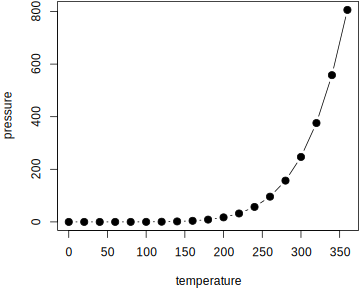
\includegraphics[width=0.5\linewidth]{bookdown_files/figure-latex/multi-plots2-1} 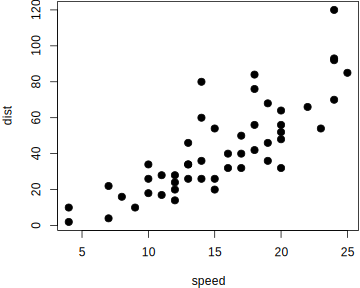
\includegraphics[width=0.5\linewidth]{bookdown_files/figure-latex/multi-plots2-2} \caption{Dos gráficos dispuestos uno al lado del otro.}\label{fig:multi-plots2}
\end{figure}

A veces es posible que tenga imágenes que no se generaron a partir de
código en R. A pesar de esto, puede incluirlas en R Markdown a través de
la función \texttt{knitr::include\_graphics()}. La figura
\ref{fig:knitr-logo2} es un ejemplo de tres logotipos de \textbf{knitr}
incluidos en un entorno gráfico. Se pueden incluir una o varias imágenes
con la función \texttt{include\_graphics()}, y todas las opciones del
chunk que se aplican a los gráficos en R también se aplican a estas
imágenes, por ejemplo, se puede usar
\texttt{out.width\ =\ \textquotesingle{}33\%\ \textquotesingle{}} para
establecer las anchuras de estas imágenes en el documento de salida.

\begin{Shaded}
\begin{Highlighting}[]
\NormalTok{knitr}\OperatorTok{::}\KeywordTok{include_graphics}\NormalTok{(}\KeywordTok{rep}\NormalTok{(}\StringTok{'images/knit-logo.png'}\NormalTok{, }\DecValTok{3}\NormalTok{))}
\end{Highlighting}
\end{Shaded}

\begin{figure}
\includegraphics[width=0.33\linewidth]{images/knit-logo} \includegraphics[width=0.33\linewidth]{images/knit-logo} \includegraphics[width=0.33\linewidth]{images/knit-logo} \caption{Tres logos de knitr incluidos en el documento desde una imagen PNG externa.}\label{fig:knitr-logo2}
\end{figure}

Las ventajas de usar \texttt{include\_graphics()} son:

\begin{enumerate}
\def\labelenumi{\arabic{enumi}.}
\tightlist
\item
  Usted no necesita preocuparse por el formato de salida de documentos,
  por ejemplo, cuando el formato de salida es LaTeX, puede que tenga que
  utilizar el comando LaTeX \texttt{\textbackslash{}includegraphics\{\}}
  para incluir una imagen, y cuando el formato de salida es Markdown,
  usted tiene que usar \texttt{!{[}{]}()}. La función
  \texttt{include\_graphics()} en \textbf{knitr} se ocupa de estos
  detalles de forma automática.
\item
  La sintaxis para el control de los atributos de la imagen es el mismo
  que cuando las imágenes se generan a partir de código en R, por
  ejemplo, las opciones del chunk \texttt{fig.cap},\texttt{out.width}, y
  \texttt{fig.show} tienen todas la misma función.
\item
  \texttt{include\_graphics()} es lo suficientemente versátil como para
  utilizar gráficos PDF de forma automática cuando el formato de salida
  es LaTeX y existen gráficos en formato PDF, por ejemplo, una ruta de
  la imagen \texttt{foo/bar.png} puede sustituirse automáticamente por
  \texttt{foo/bar.PDF} si existe esta última. Las imágenes en PDF a
  menudo tienen mejores cualidades que las imágenes de mapa de bits en
  la producción de LaTeX/PDF. Por supuesto, se puede desactivar esta
  función \texttt{include\_graphics(auto\_pdf\ =\ FALSE)}.
\item
  Se pueden escalar fácilmente estas imágenes de forma proporcional
  utilizando la misma razón. Esto se puede hacer a través del argumento
  \texttt{dpi} (puntos por pulgada), que toma el valor de la opción del
  chunk \texttt{dpi} por defecto. Si se trata de un valor numérico y la
  opción del chunk \texttt{out.width} no está establecida, el ancho de
  salida de una imagen será su anchura real (en píxeles) dividido por
  \texttt{dpi}, y sus unidades estarán en pulgadas. Por ejemplo, para
  una imagen de tamaño de 672 x 480, su anchura de salida será de 7
  pulgadas (\texttt{7in}) cuando \texttt{dpi\ =\ 96}. Esta función
  requiere del paquete \textbf{png} y/o \textbf{jpeg}. Siempre se puede
  anular el cálculo automático del ancho en pulgadas, proporcionando un
  valor no nulo a la opción del chunk \texttt{out.wdith}, o
  usar\texttt{include\_graphics(dpi\ =\ NA)}.
\end{enumerate}

\hypertarget{tablas}{\section{Tablas}\label{tablas}}

Por ahora, la forma más conveniente para generar una tabla es la función
\texttt{knitr::kable()}, porque hay algunos trucos internos en
\textbf{knitr} para que funcione con \textbf{bookdown} y los usuarios no
tienen necesidad de preocuparse por estos detalles de implementación.
Adelante se explicará cómo utilizar otros paquetes y funciones más
detalladamente en esta sección.

Al igual que las figuras, las tablas con títulos también estarán
numeradas y podrán ser referenciadas. La función \texttt{kable()}
generará automáticamente una etiqueta para un entorno de la tabla, que
es el prefijo \texttt{tab:} más la etiqueta del chunk. Por ejemplo, la
etiqueta de la tabla para un chunk con la etiqueta \texttt{foo} será:
\texttt{tab:foo}, y usar la sintaxis
\texttt{\textbackslash{}@ref(etiqueta)} para hacer referencia a la
tabla. La tabla \ref{tab:table-single} es un ejemplo sencillo.

\begin{Shaded}
\begin{Highlighting}[]
\NormalTok{knitr}\OperatorTok{::}\KeywordTok{kable}\NormalTok{(}
  \KeywordTok{head}\NormalTok{(mtcars, }\DecValTok{10}\NormalTok{), }\DataTypeTok{booktabs =} \OtherTok{TRUE}\NormalTok{,}
  \DataTypeTok{caption =} \StringTok{'Una tabla de las primeras 10 filas de la base de datos mtcars.'}
\NormalTok{)}
\end{Highlighting}
\end{Shaded}

\begin{table}

\caption{\label{tab:table-single}Una tabla de las primeras 10 filas de la base de datos mtcars.}
\centering
\begin{tabular}[t]{lrrrrrrrrrrr}
\toprule
  & mpg & cyl & disp & hp & drat & wt & qsec & vs & am & gear & carb\\
\midrule
Mazda RX4 & 21.0 & 6 & 160.0 & 110 & 3.90 & 2.620 & 16.46 & 0 & 1 & 4 & 4\\
Mazda RX4 Wag & 21.0 & 6 & 160.0 & 110 & 3.90 & 2.875 & 17.02 & 0 & 1 & 4 & 4\\
Datsun 710 & 22.8 & 4 & 108.0 & 93 & 3.85 & 2.320 & 18.61 & 1 & 1 & 4 & 1\\
Hornet 4 Drive & 21.4 & 6 & 258.0 & 110 & 3.08 & 3.215 & 19.44 & 1 & 0 & 3 & 1\\
Hornet Sportabout & 18.7 & 8 & 360.0 & 175 & 3.15 & 3.440 & 17.02 & 0 & 0 & 3 & 2\\
\addlinespace
Valiant & 18.1 & 6 & 225.0 & 105 & 2.76 & 3.460 & 20.22 & 1 & 0 & 3 & 1\\
Duster 360 & 14.3 & 8 & 360.0 & 245 & 3.21 & 3.570 & 15.84 & 0 & 0 & 3 & 4\\
Merc 240D & 24.4 & 4 & 146.7 & 62 & 3.69 & 3.190 & 20.00 & 1 & 0 & 4 & 2\\
Merc 230 & 22.8 & 4 & 140.8 & 95 & 3.92 & 3.150 & 22.90 & 1 & 0 & 4 & 2\\
Merc 280 & 19.2 & 6 & 167.6 & 123 & 3.92 & 3.440 & 18.30 & 1 & 0 & 4 & 4\\
\bottomrule
\end{tabular}
\end{table}

Si desea poner varias tablas en un único entorno de tablas, simplemente
empaquete los objetos de datos (usualmente en data frames en R) dentro
de una lista. Véase la tabla \ref{tab:table-multi} para un ejemplo. Por
favor note que esta característica está disponible únicamente para
salida HTML y PDF.

\begin{Shaded}
\begin{Highlighting}[]
\NormalTok{knitr}\OperatorTok{::}\KeywordTok{kable}\NormalTok{(}
  \KeywordTok{list}\NormalTok{(}
    \KeywordTok{head}\NormalTok{(iris[,}\DecValTok{1}\OperatorTok{:}\DecValTok{2}\NormalTok{],}\DecValTok{3}\NormalTok{),}
    \KeywordTok{head}\NormalTok{(mtcars[,}\DecValTok{1}\OperatorTok{:}\DecValTok{3}\NormalTok{],}\DecValTok{5}\NormalTok{)}
\NormalTok{  ),}
  \DataTypeTok{caption =} \StringTok{'Una trama de dos tablas.'}\NormalTok{, }\DataTypeTok{booktabs =} \OtherTok{TRUE}
\NormalTok{)}
\end{Highlighting}
\end{Shaded}

\begin{table}
\caption{\label{tab:table-multi}Una trama de dos tablas.}

\centering
\begin{tabular}[t]{rr}
\toprule
Sepal.Length & Sepal.Width\\
\midrule
5.1 & 3.5\\
4.9 & 3.0\\
4.7 & 3.2\\
\bottomrule
\end{tabular}
\centering
\begin{tabular}[t]{lrrr}
\toprule
  & mpg & cyl & disp\\
\midrule
Mazda RX4 & 21.0 & 6 & 160\\
Mazda RX4 Wag & 21.0 & 6 & 160\\
Datsun 710 & 22.8 & 4 & 108\\
Hornet 4 Drive & 21.4 & 6 & 258\\
Hornet Sportabout & 18.7 & 8 & 360\\
\bottomrule
\end{tabular}
\end{table}

Cuando no se quiera una tabla flotante en PDF, es posible utilizar el
paquete de LaTeX
\href{https://www.ctan.org/pkg/longtable}{\textbf{longtable}}, que puede
dividir una tabla a través de múltiples páginas. Para utilizar
\textbf{longtable}, sólo tiene que poner \texttt{longtable\ =\ TRUE} en
\texttt{kable()}, y asegurarse de incluir
\texttt{\textbackslash{}usepackage\{longtable\}} en el preámbulo de
LaTeX (véase la sección \ref{opciones-yaml} para saber cómo personalizar
el preámbulo LaTeX). Por supuesto, esto es irrelevante para la salida
HTML, ya que las tablas de HTML no necesitan flotar.

\begin{Shaded}
\begin{Highlighting}[]
\NormalTok{knitr}\OperatorTok{::}\KeywordTok{kable}\NormalTok{(}
\NormalTok{  iris[}\DecValTok{1}\OperatorTok{:}\DecValTok{100}\NormalTok{, ], }\DataTypeTok{longtable =} \OtherTok{TRUE}\NormalTok{, }\DataTypeTok{booktabs =} \OtherTok{TRUE}\NormalTok{,}
  \DataTypeTok{caption =} \StringTok{'Una tabla generada mediante el paquete `longtable`.'}
\NormalTok{)}
\end{Highlighting}
\end{Shaded}

\begin{longtable}[t]{rrrrl}
\caption{\label{tab:longtable}Una tabla generada mediante el paquete `longtable`.}\\
\toprule
Sepal.Length & Sepal.Width & Petal.Length & Petal.Width & Species\\
\midrule
5.1 & 3.5 & 1.4 & 0.2 & setosa\\
4.9 & 3.0 & 1.4 & 0.2 & setosa\\
4.7 & 3.2 & 1.3 & 0.2 & setosa\\
4.6 & 3.1 & 1.5 & 0.2 & setosa\\
5.0 & 3.6 & 1.4 & 0.2 & setosa\\
\addlinespace
5.4 & 3.9 & 1.7 & 0.4 & setosa\\
4.6 & 3.4 & 1.4 & 0.3 & setosa\\
5.0 & 3.4 & 1.5 & 0.2 & setosa\\
4.4 & 2.9 & 1.4 & 0.2 & setosa\\
4.9 & 3.1 & 1.5 & 0.1 & setosa\\
\addlinespace
5.4 & 3.7 & 1.5 & 0.2 & setosa\\
4.8 & 3.4 & 1.6 & 0.2 & setosa\\
4.8 & 3.0 & 1.4 & 0.1 & setosa\\
4.3 & 3.0 & 1.1 & 0.1 & setosa\\
5.8 & 4.0 & 1.2 & 0.2 & setosa\\
\addlinespace
5.7 & 4.4 & 1.5 & 0.4 & setosa\\
5.4 & 3.9 & 1.3 & 0.4 & setosa\\
5.1 & 3.5 & 1.4 & 0.3 & setosa\\
5.7 & 3.8 & 1.7 & 0.3 & setosa\\
5.1 & 3.8 & 1.5 & 0.3 & setosa\\
\addlinespace
5.4 & 3.4 & 1.7 & 0.2 & setosa\\
5.1 & 3.7 & 1.5 & 0.4 & setosa\\
4.6 & 3.6 & 1.0 & 0.2 & setosa\\
5.1 & 3.3 & 1.7 & 0.5 & setosa\\
4.8 & 3.4 & 1.9 & 0.2 & setosa\\
\addlinespace
5.0 & 3.0 & 1.6 & 0.2 & setosa\\
5.0 & 3.4 & 1.6 & 0.4 & setosa\\
5.2 & 3.5 & 1.5 & 0.2 & setosa\\
5.2 & 3.4 & 1.4 & 0.2 & setosa\\
4.7 & 3.2 & 1.6 & 0.2 & setosa\\
\addlinespace
4.8 & 3.1 & 1.6 & 0.2 & setosa\\
5.4 & 3.4 & 1.5 & 0.4 & setosa\\
5.2 & 4.1 & 1.5 & 0.1 & setosa\\
5.5 & 4.2 & 1.4 & 0.2 & setosa\\
4.9 & 3.1 & 1.5 & 0.2 & setosa\\
\addlinespace
5.0 & 3.2 & 1.2 & 0.2 & setosa\\
5.5 & 3.5 & 1.3 & 0.2 & setosa\\
4.9 & 3.6 & 1.4 & 0.1 & setosa\\
4.4 & 3.0 & 1.3 & 0.2 & setosa\\
5.1 & 3.4 & 1.5 & 0.2 & setosa\\
\addlinespace
5.0 & 3.5 & 1.3 & 0.3 & setosa\\
4.5 & 2.3 & 1.3 & 0.3 & setosa\\
4.4 & 3.2 & 1.3 & 0.2 & setosa\\
5.0 & 3.5 & 1.6 & 0.6 & setosa\\
5.1 & 3.8 & 1.9 & 0.4 & setosa\\
\addlinespace
4.8 & 3.0 & 1.4 & 0.3 & setosa\\
5.1 & 3.8 & 1.6 & 0.2 & setosa\\
4.6 & 3.2 & 1.4 & 0.2 & setosa\\
5.3 & 3.7 & 1.5 & 0.2 & setosa\\
5.0 & 3.3 & 1.4 & 0.2 & setosa\\
\addlinespace
7.0 & 3.2 & 4.7 & 1.4 & versicolor\\
6.4 & 3.2 & 4.5 & 1.5 & versicolor\\
6.9 & 3.1 & 4.9 & 1.5 & versicolor\\
5.5 & 2.3 & 4.0 & 1.3 & versicolor\\
6.5 & 2.8 & 4.6 & 1.5 & versicolor\\
\addlinespace
5.7 & 2.8 & 4.5 & 1.3 & versicolor\\
6.3 & 3.3 & 4.7 & 1.6 & versicolor\\
4.9 & 2.4 & 3.3 & 1.0 & versicolor\\
6.6 & 2.9 & 4.6 & 1.3 & versicolor\\
5.2 & 2.7 & 3.9 & 1.4 & versicolor\\
\addlinespace
5.0 & 2.0 & 3.5 & 1.0 & versicolor\\
5.9 & 3.0 & 4.2 & 1.5 & versicolor\\
6.0 & 2.2 & 4.0 & 1.0 & versicolor\\
6.1 & 2.9 & 4.7 & 1.4 & versicolor\\
5.6 & 2.9 & 3.6 & 1.3 & versicolor\\
\addlinespace
6.7 & 3.1 & 4.4 & 1.4 & versicolor\\
5.6 & 3.0 & 4.5 & 1.5 & versicolor\\
5.8 & 2.7 & 4.1 & 1.0 & versicolor\\
6.2 & 2.2 & 4.5 & 1.5 & versicolor\\
5.6 & 2.5 & 3.9 & 1.1 & versicolor\\
\addlinespace
5.9 & 3.2 & 4.8 & 1.8 & versicolor\\
6.1 & 2.8 & 4.0 & 1.3 & versicolor\\
6.3 & 2.5 & 4.9 & 1.5 & versicolor\\
6.1 & 2.8 & 4.7 & 1.2 & versicolor\\
6.4 & 2.9 & 4.3 & 1.3 & versicolor\\
\addlinespace
6.6 & 3.0 & 4.4 & 1.4 & versicolor\\
6.8 & 2.8 & 4.8 & 1.4 & versicolor\\
6.7 & 3.0 & 5.0 & 1.7 & versicolor\\
6.0 & 2.9 & 4.5 & 1.5 & versicolor\\
5.7 & 2.6 & 3.5 & 1.0 & versicolor\\
\addlinespace
5.5 & 2.4 & 3.8 & 1.1 & versicolor\\
5.5 & 2.4 & 3.7 & 1.0 & versicolor\\
5.8 & 2.7 & 3.9 & 1.2 & versicolor\\
6.0 & 2.7 & 5.1 & 1.6 & versicolor\\
5.4 & 3.0 & 4.5 & 1.5 & versicolor\\
\addlinespace
6.0 & 3.4 & 4.5 & 1.6 & versicolor\\
6.7 & 3.1 & 4.7 & 1.5 & versicolor\\
6.3 & 2.3 & 4.4 & 1.3 & versicolor\\
5.6 & 3.0 & 4.1 & 1.3 & versicolor\\
5.5 & 2.5 & 4.0 & 1.3 & versicolor\\
\addlinespace
5.5 & 2.6 & 4.4 & 1.2 & versicolor\\
6.1 & 3.0 & 4.6 & 1.4 & versicolor\\
5.8 & 2.6 & 4.0 & 1.2 & versicolor\\
5.0 & 2.3 & 3.3 & 1.0 & versicolor\\
5.6 & 2.7 & 4.2 & 1.3 & versicolor\\
\addlinespace
5.7 & 3.0 & 4.2 & 1.2 & versicolor\\
5.7 & 2.9 & 4.2 & 1.3 & versicolor\\
6.2 & 2.9 & 4.3 & 1.3 & versicolor\\
5.1 & 2.5 & 3.0 & 1.1 & versicolor\\
5.7 & 2.8 & 4.1 & 1.3 & versicolor\\
\bottomrule
\end{longtable}

Puede usar cualquier tipo de tablas de Markdown en su documento. Para
poder hacer una referencia cruzada de una tabla de Markdown, debe tener
un título etiquetado de la forma
\texttt{Table:\ (\textbackslash{}\#label)\ Leyenda\ aquí}, donde la
etiqueta debe tener el prefijo: \texttt{tab}, por ejemplo,
\texttt{tab:\ simple-table}.

Si decide utilizar otros paquetes para generar tablas, tiene que
asegurarse de que la etiqueta para el ambiente de la tabla aparezca al
comienzo de la leyenda de la tabla de la forma
\texttt{(\textbackslash{}\#label)}, donde \texttt{label} debe tener el
prefijo \texttt{tab:}. Tiene que tenerse mucho cuidado con la
\emph{portabilidad} de la función que genera la tabla: deberá trabajar
tanto para la salida HTML como para LaTeX de forma automática, por lo
que debe tener en cuenta el formato de salida internamente (revise
\texttt{knitr::opts\_knit\$get(\textquotesingle{}pandoc.to\textquotesingle{})}).
Al escribir una tabla HTML, el título debe ser escrito en la etiqueta
\texttt{\textless{}caption\textgreater{}\textless{}/caption\textgreater{}}.
Para las tablas simples, \texttt{kable()} debería ser suficiente. Si
usted tiene que crear tablas complicadas (por ejemplo, con ciertas
celdas que atraviesen múltiples columnas/filas), tendrá que tomar las
cuestiones mencionadas en consideración.

\section{Referencias cruzadas}\label{referencias-cruzadas}

Se ha explicado cómo funcionan las referencias cruzadas para ecuaciones
(Sección \ref{ecuaciones}), teoremas (Sección \ref{teoremas}), figuras
(Sección \ref{figuras}) y tablas (Sección \ref{tablas}). De hecho,
también se puede hacer referencia a secciones utilizando la misma
sintaxis \texttt{\textbackslash{}@ref(label)}, donde \texttt{label} es
el identificador de una sección. De forma predeterminada, Pandoc
generará un ID para todos los encabezados de sección, por ejemplo, una
sección \texttt{\#\ Hola\ Mundo} tendrá un ID \texttt{hola-mundo}. Se
recomienda asignar manualmente un identificador para un encabezado de
sección con el fin de asegurarse de que no se olvide actualizar la
etiqueta de referencia después de cambiar el encabezado de sección. Para
asignar un ID a un encabezado de sección, simplemente añada
\texttt{\{\#id\}} hasta el final del encabezado de sección.

Cuando una etiqueta referenciada no se puede encontrar, verá dos signos
de interrogación como \ref{fig:no-existe}, así como un mensaje de
advertencia en la consola de R cuando se compila el libro.

También pueden crearse enlaces basados en texto usando identificadores
de sección explícita o automáticos e incluso el texto del encabezado de
sección actual.

\begin{itemize}
\tightlist
\item
  Si usted está satisfecho con el encabezado de sección como texto de
  enlace, úselo dentro de un único conjunto de paréntesis cuadrados:

  \begin{itemize}
  \tightlist
  \item
    \texttt{{[}Texto\ en\ la\ sección\ de\ encabezado{]}}: ejemplo
    ``\protect\hyperlink{un-documento-sencillo}{Un documento sencillo}''
    a través de \texttt{{[}Un\ documento\ sencillo{]}}
  \end{itemize}
\item
  Hay dos formas de especificar el texto del vínculo personalizado:

  \begin{itemize}
  \tightlist
  \item
    \texttt{{[}Texto\ del\ vínculo{]}{[}Sección\ texto\ de\ encabezado{]}}:
    \protect\hyperlink{internacionalizacion}{los libros que no están en
    inglés} a través de
    \texttt{{[}libros\ no\ están\ en\ inglés{]}\ {[}Internacionalización{]}}
  \item
    \texttt{{[}Texto\ del\ enlace{]}\ (\#ID)}:
    ``\protect\hyperlink{tablas}{Tabla cosas}'' a través de
    \texttt{{[}Tabla\ cosas{]}(\#tablas)}
  \end{itemize}
\end{itemize}

La documentación acerca de Pandoc proporciona más detalles sobre
\href{http://pandoc.org/README.html\#extension-auto_identifiers}{identificación
automática de secciones} y
\href{http://pandoc.org/README.html\#extension-\%20implicit_header_references}{referencias
de cabecera implícitas}.

Las referencias cruzadas siguen funcionando incluso cuando se refiere a
un item que no esté en la página actual de la salida PDF o HTML. Por
ejemplo, véase la ecuación \eqref{eq:binom} y la figura
\ref{fig:knitr-logo2}

\section{Bloques personalizados}\label{bloques-personalizados}

Puede generar bloques personalizados \index{bloques personalizado}
utilizando el motor de \texttt{block} en \textbf{knitr} , es decir, la
opción del chunk
\texttt{engine\ =\ \textquotesingle{}block\textquotesingle{}}, o la
sintaxis más compacta
\texttt{\textasciigrave{}\textasciigrave{}\textasciigrave{}\{block\}}.
Este motor se debe utilizar en combinación con la opción del chunk
\texttt{type}, que tiene una cadena de caracteres. Cuando se utiliza el
motor de \texttt{block}, genera un \texttt{\textless{}div\textgreater{}}
para envolver el contenido del chunk si el formato de salida es HTML, y
un entorno de LaTeX si la salida es ésta. La opción \texttt{type}
especifica la clase del \texttt{\textless{}div\textgreater{}} y el
nombre del entorno de LaTeX. Por ejemplo, la salida HTML de este chunk

\begin{verbatim}
```{block, type='FOO'}
Some text for this block.
```
\end{verbatim}

sería:

\begin{Shaded}
\begin{Highlighting}[]
\KeywordTok{<div}\OtherTok{ class=}\StringTok{"FOO"}\KeywordTok{>}
\NormalTok{Some text for this block.}
\KeywordTok{</div>}
\end{Highlighting}
\end{Shaded}

y la salida en LaTeX sería:

\begin{Shaded}
\begin{Highlighting}[]
\KeywordTok{\textbackslash{}begin}\NormalTok{\{}\ExtensionTok{FOO}\NormalTok{\}}
\NormalTok{Some text for this block.}
\KeywordTok{\textbackslash{}end}\NormalTok{\{}\ExtensionTok{FOO}\NormalTok{\}}
\end{Highlighting}
\end{Shaded}

Depende del autor del libro establecer cómo definir el estilo del
bloque. Puede definir el estilo de \texttt{\textless{}div\textgreater{}}
en CSS e incluirlo en la salida a través de la opción \texttt{includes}
en los metadatos YAML. Del mismo modo, puede definir el entorno de LaTeX
a través de \texttt{\textbackslash{}newenvironment} e incluir la
definición en la salida de LaTeX a través de la opción
\texttt{includes}. Por ejemplo, podemos guardar el siguiente estilo en
un archivo CSS, digamos, \texttt{style.css}:

\begin{Shaded}
\begin{Highlighting}[]
\NormalTok{div}\FloatTok{.FOO} \KeywordTok{\{}
  \KeywordTok{font-weight:} \DataTypeTok{bold}\KeywordTok{;}
  \KeywordTok{color:} \DataTypeTok{red}\KeywordTok{;}
\KeywordTok{\}}
\end{Highlighting}
\end{Shaded}

Y los metadatos YAML del documento R Markdown pueden ser:

\begin{Shaded}
\begin{Highlighting}[]
\OtherTok{---}
\FunctionTok{output:}
  \FunctionTok{bookdown:}\AttributeTok{:html_book:}
    \FunctionTok{includes:}
      \FunctionTok{in_header:}\AttributeTok{ style.css}
\OtherTok{---}
\end{Highlighting}
\end{Shaded}

Hemos definido algunos tipos de bloques para que este libro muestre
notas, consejos y advertencias, etc. A continuación se presentan algunos
ejemplos:

\BeginKnitrBlock{rmdnote}
R es software libre y viene con ABSOLUTAMENTE NINGUNA GARANTÍA. Le
invitamos a redistribuirlo bajo los términos de la GNU General Public
License versiones 2 o 3. Para más información sobre estos asuntos,
\url{http://www.gnu.org/licenses/}.
\EndKnitrBlock{rmdnote}

\BeginKnitrBlock{rmdcaution}
R es software libre y viene con ABSOLUTAMENTE NINGUNA GARANTÍA. Le
invitamos a redistribuirlo bajo los términos de la GNU General Public
License versiones 2 o 3. Para más información sobre estos asuntos,
\url{http://www.gnu.org/licenses/}.
\EndKnitrBlock{rmdcaution}

\BeginKnitrBlock{rmdimportant}
R es software libre y viene con ABSOLUTAMENTE NINGUNA GARANTÍA. Le
invitamos a redistribuirlo bajo los términos de la GNU General Public
License versiones 2 o 3. Para más información sobre estos asuntos,
\url{http://www.gnu.org/licenses/}.
\EndKnitrBlock{rmdimportant}

\BeginKnitrBlock{rmdtip}
R es software libre y viene con ABSOLUTAMENTE NINGUNA GARANTÍA. Le
invitamos a redistribuirlo bajo los términos de la GNU General Public
License versiones 2 o 3. Para más información sobre estos asuntos,
\url{http://www.gnu.org/licenses/}.
\EndKnitrBlock{rmdtip}

\BeginKnitrBlock{rmdwarning}
R es software libre y viene con ABSOLUTAMENTE NINGUNA GARANTÍA. Le
invitamos a redistribuirlo bajo los términos de la GNU General Public
License versiones 2 o 3. Para más información sobre estos asuntos,
\url{http://www.gnu.org/licenses/}.
\EndKnitrBlock{rmdwarning}

El motor \textbf{knitr} \texttt{block} fue diseñado para mostrar
contenido simple (normalmente un párrafo de texto sin formato). Puede
utilizar una sintaxis de formato simple, como hacer que ciertas palabras
sean negritas o cursivas, pero la sintaxis más avanzada, como las citas
y las referencias cruzadas, no funcionarán. Sin embargo, hay un motor
alternativo denominado \texttt{block2} que soporta la sintaxis
arbitraria de Markdown, por ejemplo,

\begin{Shaded}
\begin{Highlighting}[]
\NormalTok{```\{block2, type='FOO'\}}
\NormalTok{Some text for this block [@citation-key].}

\NormalTok{- }\FloatTok{a list item}
\FloatTok{- another item}

\NormalTok{More text.}
\NormalTok{```}
\end{Highlighting}
\end{Shaded}

El motor \texttt{block2} también debería ser más rápido que el motor
\texttt{block} si tiene muchos bloques personalizados en el documento,
pero su implementación se basó en
\href{https://github.com/jgm/pandoc/issues/2453}{un hack,} por lo que no
estamos 100\% seguros de si siempre va a funcionar en el futuro. No
hemos visto problemas con Pandoc v1.17.2 todavía.

Una advertencia más para el motor \texttt{block2}: si el último elemento
del bloque no es un párrafo ordinario, debe dejar una línea en blanco al
final, por ejemplo,

\begin{Shaded}
\begin{Highlighting}[]
\NormalTok{```\{block2, type='FOO'\}}
\NormalTok{Some text for this block [@citation-key].}

\NormalTok{- }\FloatTok{a list item}
\FloatTok{- another item}
\FloatTok{- end the list with a blank line}

\NormalTok{```}
\end{Highlighting}
\end{Shaded}

El teorema y los entornos de prueba en la sección \ref{teoremas} se
implementan en realidad a través del motor \texttt{block2}.

Para todos los bloques personalizados basados en el motor \texttt{block}
o \texttt{block2}, hay una opción de bloqueo \texttt{echo} que puede
usar para mostrar (\texttt{echo\ =\ TRUE}) u ocultar
(\texttt{echo\ =\ FALSE}) los bloques.

\section{Citas}\label{citas}

Aunque Pandoc soporta múltiples formas de escribir las citas, se
recomienda que utilice las bases de datos BibTeX porque trabajan mejor
con la salida de LaTeX/PDF. Pandoc puede procesar otros tipos de bases
de datos bibliográficas con la utilidad \texttt{pandoc-citeproc}
(\url{https://github.com/jgm/pandoc-citeproc}), pero no pone ciertos
elementos de bibliografía correctamente (especialmente en el caso de
múltiples autores). Con las bases de datos BibTeX, podrá definirse el
estilo bibliográfico si se requiere por un determinado editor o revista.

Una base de datos BibTeX es un archivo de texto (con la extensión de
nombre de archivo convencional \texttt{.bib}) que consta de entradas
bibliográficas como:

\begin{Shaded}
\begin{Highlighting}[]
\VariableTok{@Manual}\NormalTok{\{}\OtherTok{R}\NormalTok{-}\OtherTok{base}\NormalTok{,}
  \DataTypeTok{title}\NormalTok{ = \{R: A Language and Environment for Statistical Computing\},}
  \DataTypeTok{author}\NormalTok{ = \{\{R Core Team\}\},}
  \DataTypeTok{organization}\NormalTok{ = \{R Foundation for Statistical Computing\},}
  \DataTypeTok{address}\NormalTok{ = \{Vienna, Austria\},}
  \DataTypeTok{year}\NormalTok{ = \{2015\},}
  \DataTypeTok{url}\NormalTok{ = \{https://www.R-project.org/\},}
\NormalTok{\}}
\end{Highlighting}
\end{Shaded}

Una entrada bibliográfica comienza con \texttt{\{@type}, donde
\texttt{type} puede ser \texttt{article}, \texttt{book},\texttt{manual},
etc.\footnote{El nombre del tipo no diferencia mayúsculas y minúsculas,
  por ende no importa si es \texttt{manual}, \texttt{Manual}, o
  \texttt{MANUAL}.}. A continuación hay una clave de citación, como
\texttt{R-base} en el ejemplo anterior. Para citar una entrada, use
\texttt{@\ key} o \texttt{{[}@key{]}} (este último pone la cita entre
paréntesis), por ejemplo, \texttt{@R-base} se compila como
\citet{R-base}, y \texttt{{[}@\ R-base{]}} genera ``\citep{R-base}''. Si
no está familiarizado con el paquete \textbf{natbib} de LaTeX,
\texttt{@key} es básicamente \texttt{\textbackslash{}citet\{key\}} y
\texttt{{[}@key{]}} es equivalente a
\texttt{\textbackslash{}citep\{key\}}.

Hay una serie de campos en una entrada de bibliografía, tales como
\texttt{title}, \texttt{author}, y \texttt{year}, etc. Puede visitar
\url{https://en.wikipedia.org/wiki/BibTeX} para saber más sobre posibles
tipos de entradas y campos en BibTeX.

Hay una función auxiliar \texttt{write\_bib()} en \textbf{knitr} para
generar entradas BibTeX automáticamente para paquetes en R. Tenga en
cuenta que sólo genera una entrada de BibTeX para el propio paquete en
el momento, mientras que un paquete puede contener múltiples entradas en
el archivo \texttt{CITATION}, y algunas entradas versan sobre las
publicaciones relacionadas con el paquete. Estas entradas son ignoradas
por \texttt{write\_bib()}.

\begin{Shaded}
\begin{Highlighting}[]
\CommentTok{# el segundo argumento puede ser un archivo .bib}
\NormalTok{knitr}\OperatorTok{::}\KeywordTok{write_bib}\NormalTok{(}\KeywordTok{c}\NormalTok{(}\StringTok{'knitr'}\NormalTok{, }\StringTok{'stringr'}\NormalTok{), }\StringTok{''}\NormalTok{)}
\end{Highlighting}
\end{Shaded}

\begin{verbatim}
@Manual{R-knitr,
  title = {knitr: A General-Purpose Package for Dynamic Report Generation in R},
  author = {Yihui Xie},
  year = {2017},
  note = {R package version 1.18},
  url = {https://CRAN.R-project.org/package=knitr},
}
@Manual{R-stringr,
  title = {stringr: Simple, Consistent Wrappers for Common String Operations},
  author = {Hadley Wickham},
  year = {2017},
  note = {R package version 1.2.0},
  url = {https://CRAN.R-project.org/package=stringr},
}
\end{verbatim}

Una vez que tenga uno o varios archivos \texttt{.bib}, puede utilizar el
campo \texttt{bibliography} en los metadatos del documento YAML del
documento R Markdown, y también se puede especificar el estilo de
bibliografía a través de \texttt{biblio-style} (esto sólo se aplica a
las salidas en PDF), por ejemplo,

\begin{Shaded}
\begin{Highlighting}[]
\OtherTok{---}
\FunctionTok{bibliography:}\AttributeTok{ }\KeywordTok{[}\StringTok{"one.bib"}\KeywordTok{,} \StringTok{"another.bib"}\KeywordTok{,} \StringTok{"yet-another.bib"}\KeywordTok{]}
\FunctionTok{biblio-style:}\AttributeTok{ }\StringTok{"apalike"}
\FunctionTok{link-citations:}\AttributeTok{ true}
\OtherTok{---}
\end{Highlighting}
\end{Shaded}

El campo \texttt{link-citations} se puede utilizar para añadir enlaces
internos a partir del texto de la cita del estilo autor-año de la
entrada bibliográfica en la salida HTML.

Cuando el formato de salida es LaTeX, las citas se colocarán
automáticamente en un capítulo o sección. Para la salida no LaTeX, puede
agregar un capítulo vacío como el último capítulo de su libro. Por
ejemplo, si su último capítulo es el archivo Rmd
\texttt{06-references.Rmd}, su contenido puede ser una expresión R en
línea:

\begin{Shaded}
\begin{Highlighting}[]
\BaseNTok{`r if (knitr:::is_html_output()) '# References \{-\}'`}
\end{Highlighting}
\end{Shaded}

\section{Índices}\label{latex-index}

Actualmente el índice \index{index} sólo se admite para la producción de
LaTeX/PDF. Para imprimir un índice después del libro, puede utilizar el
paquete de LaTeX \textbf{makeindex} en el preámbulo (véase la sección
\ref{opciones-yaml}):

\begin{Shaded}
\begin{Highlighting}[]
\BuiltInTok{\textbackslash{}usepackage}\NormalTok{\{}\ExtensionTok{makeidx}\NormalTok{\}}
\FunctionTok{\textbackslash{}makeindex}
\end{Highlighting}
\end{Shaded}

A continuación, inserte \texttt{\textbackslash{}printindex} al final de
su libro a través de la opción YAML
\texttt{includes\ -\textgreater{}\ after\_body}. Una entrada de índice
se puede crear a través del comando \texttt{\textbackslash{}\{index\}}
en el cuerpo del libro, por ejemplo,
\texttt{\textbackslash{}index\{GIT\}}.

\section{HTML Widgets}\label{html-widgets}

Aunque una de las mayores fortalezas de R es la visualización de datos,
hay un gran número de librerías de JavaScript para la visualización de
datos mucho más rica. Estas librerías se pueden utilizar para crear
aplicaciones interactivas que pueden procesarse fácilmente en los
navegadores web, por lo que los usuarios no necesitan instalar ningún
paquete de software adicional para ver las visualizaciones. Una forma de
llevar estas librerías JavaScript a R es a través del paquete
\href{http://htmlwidgets.org}{\textbf{htmlwidgets}}
\citep{R-htmlwidgets}\index{HTML widget}.

Los HTML widgets pueden representarse como una página web independiente
(al igual que un gráfico de R), o incrustarse en los documentos de R
Markdown y aplicaciones Shiny. Fueron diseñados originalmente para
salidas HTML solamente, y requieren la disponibilidad de JavaScript, por
lo que no van a trabajar en formatos que no son HTML de salida, tales
como LaTeX/PDF. Antes de la v1.13 de \textbf{knitr}, se obtenía un error
cuando se procesaban widgets de HTML a un formato de salida que no era
HTML. A partir de esta versión, los widgets de HTML se procesan
automáticamente como imágenes tomadas a través del paquete
\textbf{webshot} \citep{R-webshot}. Por supuesto, es necesario instalar
el paquete \textbf{webshot}. Además, debe instalarse PhantomJS
(\url{http://phantomjs.org}), ya que es lo que \textbf{webshot} utiliza
para capturar imágenes. Tanto \textbf{WebShot} como PhantomJS se pueden
instalar de forma automática desde R:

\begin{Shaded}
\begin{Highlighting}[]
\KeywordTok{install.packages}\NormalTok{(}\StringTok{'webshot'}\NormalTok{)}
\NormalTok{webshot}\OperatorTok{::}\KeywordTok{install_phantomjs}\NormalTok{()}
\end{Highlighting}
\end{Shaded}

La función \texttt{install\_phantomjs()} funciona para Windows, OSX, y
Linux. También puede optar por descargar e instalar PhantomJS por sí
mismo, si está familiarizado con la modificación del entorno del sistema
variable de \texttt{PATH}.

Cuando \textbf{knitr} detecta un objeto widget de HTML en un chunk, o
compila el widget normalmente cuando el formato de salida actual es
HTML, o guarda el widget como una página HTML y llama a \textbf{webshot}
para capturar la pantalla de la página HTML cuando el formato de salida
no es HTML. He aquí un ejemplo de una tabla creada a partir del paquete
\textbf{DT} \citep{R-DT}:

\begin{Shaded}
\begin{Highlighting}[]
\NormalTok{DT}\OperatorTok{::}\KeywordTok{datatable}\NormalTok{(iris)}
\end{Highlighting}
\end{Shaded}

\hypertarget{htmlwidget-e1294e847e7b96ffa195}{}

\label{fig:DT-demo}Una tabla widget compilada a través del paquete DT.

Si usted está leyendo este libro como un página web ahora mismo, debería
ver una tabla interactiva generada a partir del chunk anterior, por
ejemplo, puede ordenar las columnas y generar la búsqueda en la tabla.
Si está leyendo una versión que no sea HTML de este libro, debería ver
una captura de pantalla de la tabla. La captura de pantalla puede tener
un aspecto un poco diferente con el widget real mostrado en el navegador
web, debido a la diferencia entre un navegador web real y navegador
virtual PhantomJS '.

Hay un número de opciones de chunk de \textbf{knitr} relacionados con la
captura de pantalla. En primer lugar, si usted no está satisfecho con la
calidad de las capturas de pantalla automáticas, o desea una captura de
pantalla del widget en un estado en particular (por ejemplo, después de
hacer clic y ordenar una determinada columna de una tabla), puede
capturar la pantalla de forma manual, y proporcionar su propia captura a
través de la opción del chunk \texttt{screenshot.alt} (capturas de
pantalla alternativas). Esta opción toma las ubicaciones de las
imágenes. Si tiene varios widgets en un chunk, se puede proporcionar un
vector con las rutas de las imágenes. Cuando esta opción está presente,
\textbf{knitr} ya no llamará a \textbf{webshot} para tomar capturas de
pantalla automáticas.

En segundo lugar, a veces es posible que desee forzar a \textbf{knitr} a
utilizar imágenes estáticas en lugar de compilar los widgets incluso en
páginas HTML. En este caso, se puede establecer la opción del chunk
\texttt{screenshot.force\ =\ TRUE}, y los widgets siempre serán
mostrados como imágenes estáticas. Debe tenerse en cuenta que aún puede
optar por utilizar capturas de pantalla automáticas o personalizadas.

En tercer lugar, \textbf{webshot} tiene algunas opciones para controlar
las capturas de pantalla automáticas, y es posible especificar estas
opciones a través de la opción en el chunk \texttt{screenshot.opts}, que
toma una lista como
\texttt{list(delay\ =\ 2,\ cliprect\ =\ \textquotesingle{}viewport\textquotesingle{})}.
Ver la página de ayuda \texttt{?} \texttt{webshot::webshot} para la
lista completa de posibles opciones, y la
\href{https://cran.rstudio.com/web/packages/webshot/vignettes/intro.html}{viñeta
del paquete}
\texttt{vignette(\textquotesingle{}intro\textquotesingle{},\ package\ =\ \textquotesingle{}webshot\textquotesingle{})}
ha ilustrado el efecto de estas opciones. Aquí la opción \texttt{delay}
puede ser importante para los widgets que toman mucho tiempo en
cargarse: \texttt{delay} especifica el número de segundos de espera
antes de que PhantomJS capture la pantalla. Si ve una pantalla
incompleta, es posible que desee especificar un retraso más largo (el
valor predeterminado es 0,2 segundos).

En cuarto lugar, si usted siente que esto es lento para capturar las
imágenes, o no quieren hacerlo cada vez que ejecuta el chunk, se puede
utilizar la opción del chunk \texttt{cache\ =\ TRUE} para almacenar en
caché el chunk. El almacenamiento en caché funciona tanto para HTML como
para formatos de salida que no son HTML.

Las imágenes se comportan como gráficos normales en R en el sentido de
que muchas opciones del chunk relacionadas con figuras también se
aplican a las capturas, incluyendo
\texttt{fig.width},\texttt{fig.height}, \texttt{out.width},
\texttt{fig.cap}, etc. Así pues, puede especificarse el tamaño de las
capturas de pantalla en el documento de salida, y asignar los pies de
figura a ellos también. El formato de imagen de las capturas de pantalla
automáticas puede especificarse mediante la opción \texttt{dev}, y los
posibles valores son \texttt{PDF}, \texttt{png}, y \texttt{jpeg}. El
valor predeterminado para la salida PDF es \texttt{PDF}, y \texttt{png}
para otros tipos de salida. Nótese que \texttt{PDF} puede no funcionar
tan fielmente como \texttt{png}: a veces hay ciertos elementos en una
página HTML que no puede representarse en la captura de pantalla en PDF,
por lo que es posible que desee utilizarse
\texttt{dev\ =\ \textquotesingle{}png\textquotesingle{}} incluso para la
salida PDF. Depende de los casos específicos de widgets de HTML, y se
puede intentar tanto \texttt{PDF} como \texttt{png} (o \texttt{jpeg})
antes de decidir qué formato es el más deseable.

\section{Páginas web y aplicaciones
Shiny}\label{paginas-web-y-aplicaciones-shiny}

Al igual que en los HTML widgets, los sitios web se pueden incrustar en
el libro. Puede utilizar la función \texttt{knitr::include\_url()} para
incluir una página web a través de su URL. Cuando el formato de salida
es HTML, se usa un \texttt{iframe}\footnote{Un \texttt{iframe} es
  básicamente una caja en una página Web para incrustar otra página Web.};
en otros casos, \textbf{knitr} trata de tomar una captura de pantalla de
la página web (o utilizar una captura de pantalla personalizada en la
medida en que se haya pensado). Todas las opciones del chunk son las
mismas que para los HTML widgets. Una opción que puede requerir atención
especial es la opción \texttt{delay}: los HTML widgets se compilan a
nivel local, por lo que por lo general son rápidos para cargar por
PhantomJS para tomar capturas de pantalla, pero una URL arbitraria
pueden tardar más tiempo en cargarse, por lo que es posible que desee
utilizar un valor mayor de \texttt{delay}, por ejemplo, utilizar la
opción del chunk \texttt{screenshot.opts\ =\ list(delay\ =\ 5)}.

Una función relacionada es \texttt{knitr::include\_app()}, que es muy
similar a \texttt{include\_url()}, y fue diseñada para incrustar
aplicaciones shiny a través de sus direcciones URL en la salida. Su
única diferencia con \texttt{include\_url()} es que añade
automáticamente un parámetro de consulta \texttt{?showcase=0} a la URL,
si no hay otros parámetros de consulta que estén presentes en la URL,
desactiva el modo showcase de Shiny, lo que es poco probable que sea
útil para las capturas de pantalla o iframes. Si se desea solo el modo
showcase, únicamente use \texttt{include\_url()} en lugar de
\texttt{include\_app()}. A continuación se muestra un ejemplo de
aplicación Shiny (Figura \ref{fig:miniUI}):

\let\ooldhref\href
\let\href\oldhref

\begin{Shaded}
\begin{Highlighting}[]
\NormalTok{knitr}\OperatorTok{::}\KeywordTok{include_app}\NormalTok{(}\StringTok{'https://yihui.shinyapps.io/miniUI/'}\NormalTok{, }\DataTypeTok{height =} \StringTok{'600px'}\NormalTok{)}
\end{Highlighting}
\end{Shaded}

\label{fig:miniUI}Una aplicación en Shiny creada mediante el paquete miniUI;
puede ver una versiòn en vivo en:
\url{https://yihui.shinyapps.io/miniUI/}.

\let\href\ooldhref

Una vez más, verá una aplicación en vivo si está leyendo una versión
HTML de este libro, y una captura de pantalla estática si está leyendo
otros tipos de formatos. La aplicación Shiny anterior se ha creado
usando el paquete \textbf{miniUI} \citep{R-miniUI}, que proporciona
funciones de diseño que son particularmente agradables para aplicaciones
Shiny en pantallas pequeñas. Si utiliza funciones de diseño Shiny
normales, es probable que vea las barras de desplazamiento verticales
y/o horizontales en los marcos flotantes debido a que el tamaño de
página es demasiado grande para caber un marco flotante. Cuando el ancho
predeterminado del marco flotante es demasiado pequeño, puede utilizar
la opción del chunk \texttt{out.width} para cambiarlo. Para la altura
del iframe, utilice el argumento \texttt{height} característica de
\texttt{include\_url()} / \texttt{include\_app()}.

Las aplicaciones Shiny pueden tardar más tiempo en cargar que las URL
habituales. Es posible que desee utilizar un valor conservador para la
opción \texttt{delay}, por ejemplo, 10. Es evidente que tanto
\texttt{include\_url()} como \texttt{include\_app()} requieren conexión
a Internet, a menos que haya almacenado en caché previamente el chunk
(pero páginas Web dentro de iframes aún no funcionan sin una conexión a
Internet).

\chapter{Formatos de salida}\label{formatos-de-salida}

El paquete \textbf{bookdown} es compatible principalmente con tres tipos
de formatos de salida: HTML, LaTeX/PDF y e-books. En este capítulo
presentamos las opciones posibles para estos formatos. Los formatos de
salida pueden especificarse en los metadatos YAML del primer archivo Rmd
del libro o en un archivo YAML por separado llamado
\texttt{\_output.yml} que se encuentra en el directorio raíz del libro.
Un breve ejemplo de los primeros (los formatos de salida que se
especifican en el campo \texttt{output} de los metadatos YAML) es:

\begin{Shaded}
\begin{Highlighting}[]
\OtherTok{---}
\FunctionTok{title:}\AttributeTok{ }\StringTok{"Un libro impresionante"}
\FunctionTok{author:}\AttributeTok{ }\StringTok{"Martín Macías y Prof. Daniel Rodríguez"}
\FunctionTok{output:}
  \FunctionTok{bookdown:}\AttributeTok{:gitbook:}
    \FunctionTok{lib_dir:}\AttributeTok{ assets}
    \FunctionTok{split_by:}\AttributeTok{ section}
    \FunctionTok{config:}
      \FunctionTok{toolbar:}
        \FunctionTok{position:}\AttributeTok{ static}
  \FunctionTok{bookdown:}\AttributeTok{:pdf_book:}
    \FunctionTok{keep_tex:}\AttributeTok{ yes}
  \FunctionTok{bookdown:}\AttributeTok{:html_book:}
    \FunctionTok{css:}\AttributeTok{ toc.css}
\FunctionTok{documentclass:}\AttributeTok{ book}
\OtherTok{---}
\end{Highlighting}
\end{Shaded}

Un ejemplo del archivo \texttt{\_output.yml} es:

\begin{Shaded}
\begin{Highlighting}[]
\FunctionTok{bookdown:}\AttributeTok{:gitbook:}
  \FunctionTok{lib_dir:}\AttributeTok{ assets}
  \FunctionTok{split_by:}\AttributeTok{ section}
  \FunctionTok{config:}
    \FunctionTok{toolbar:}
      \FunctionTok{position:}\AttributeTok{ static}
\FunctionTok{bookdown:}\AttributeTok{:pdf_book:}
  \FunctionTok{keep_tex:}\AttributeTok{ yes}
\FunctionTok{bookdown:}\AttributeTok{:html_book:}
  \FunctionTok{css:}\AttributeTok{ toc.css}
\end{Highlighting}
\end{Shaded}

En este caso, todos los formatos deben estar en el nivel superior, en
vez de estar bajo un campo \texttt{output}. En el archivo
\texttt{\_output.yml} no necesita usar tres guiones \texttt{-\/-\/-} .

\section{HTML}\label{html}

La principal diferencia entre compilar un libro (usando
\textbf{bookdown}) y compilar un simple documento R Markdown (utilizando
\textbf{rmarkdown}) a HTML es que un libro generará múltiples páginas
HTML de forma predeterminada --- normalmente un archivo HTML por
capítulo. Esto hace que sea más fácil de señalar un determinado capítulo
o compartir su URL con otras personas a medida que se lee el libro,
además de ser más rápido a la hora de cargar el libro en el navegador
web. Actualmente se ha proporcionado un número de estilos diferentes
para la salida HTML: el estilo GitBook, el estilo Bootstrap, y el estilo
Tufte.

\subsection{El estilo GitBook}\label{estilo-gitbook}

El estilo GitBook fue tomado de GitBook, un proyecto puesto en marcha
por Friendcode, Inc (\url{https://www.gitbook.com}) y se dedica a ayudar
a los autores a escribir libros con Markdown. Proporciona un estilo
bonito, con un diseño que consiste en una barra lateral que muestra la
tabla de contenido en la parte izquierda de la pantalla, y el cuerpo
principal del libro a la derecha. El diseño es sensible al tamaño de la
ventana, por ejemplo, los botones de navegación se muestran a la
izquierda/derecha del cuerpo del libro cuando la ventana es lo
suficientemente ancha, y colapsa en la parte inferior cuando la ventana
es estrecha para dar a los lectores más espacio horizontal para leer el
cuerpo del libro.

Se han hecho varias mejoras con respecto al proyecto original GitBook.
El más significativo es que se ha sustituido el motor de Markdown con R
Markdown v2 basado en Pandoc, por lo que hay muchas más características
para utilizar cuando se escribe un libro. Por ejemplo,

\begin{itemize}
\tightlist
\item
  Puede incorporar chunks en R y expresiones en línea de R en Markdown,
  y esto hace que sea fácil crear documentos reproducibles y lo libera
  de sincronizar su cómputo con la salida actual (\textbf{knitr} se
  encargará de eso automáticamente);
\item
  La sintaxis de Markdown es mucho más rica: se puede escribir cualquier
  cosa que Markdown de Pandoc soporte, como las expresiones matemáticas
  de LaTeX y citas;
\item
  Puede incrustar contenido interactivo en el libro (para la salida HTML
  únicamente), tales como HTML widgets y aplicaciones Shiny;
\end{itemize}

También se han añadido algunas características útiles en la interfaz de
usuario que se introducirán en detalle a continuación. La función de
formato de salida para el estilo GitBook en \textbf{bookdown} es
\texttt{gitbook()}. A continuación se presentan sus argumentos:

\begin{Shaded}
\begin{Highlighting}[]
\KeywordTok{gitbook}\NormalTok{(}\DataTypeTok{fig_caption =} \OtherTok{TRUE}\NormalTok{, }\DataTypeTok{number_sections =} \OtherTok{TRUE}\NormalTok{,}
  \DataTypeTok{self_contained =} \OtherTok{FALSE}\NormalTok{, }\DataTypeTok{lib_dir =} \StringTok{"libs"}\NormalTok{, ...,}
  \DataTypeTok{split_by =} \KeywordTok{c}\NormalTok{(}\StringTok{"chapter"}\NormalTok{, }\StringTok{"chapter+number"}\NormalTok{, }\StringTok{"section"}\NormalTok{, }\StringTok{"section+number"}\NormalTok{, }\StringTok{"rmd"}\NormalTok{, }\StringTok{"none"}\NormalTok{),}
  \DataTypeTok{split_bib =} \OtherTok{TRUE}\NormalTok{, }\DataTypeTok{config =} \KeywordTok{list}\NormalTok{())}
\end{Highlighting}
\end{Shaded}

La mayoría de los argumentos se pasan a
\texttt{rmarkdown::html\_document()}, incluyendo \texttt{fig\_caption},
\texttt{lib\_dir}, y \texttt{...} . Puede comprobarse en la página de
ayuda de \texttt{rmarkdown::html\_document()}, la lista completa de
opciones posibles. Se recomienda encarecidamente utilizar
\texttt{fig\_caption\ =\ TRUE} por dos razones: 1) Es importante
explicar las figuras con etiquetas; 2) permitir que los pies de figura
representen figuras que se colocarán en entornos flotantes cuando la
salida sea LaTeX, de lo contrario puede terminar con una gran cantidad
de espacio en blanco en ciertas páginas. El formato de los números de
figura/tabla depende de si las secciones están numeradas o no: si
\texttt{number\_sections\ =\ TRUE}, estos números serán del
formato\texttt{X.i}, donde \texttt{X} es el número del capítulo, e
\texttt{i} es un incremento numérico; si las secciones no están
numeradas, todas las figuras/tablas serán numeradas secuencialmente a
través del libro de 1, 2, \ldots{}, N. Note que en cualquiera de los
casos, las figuras y tablas se numerarán de forma independiente.

Entre todos los argumentos posibles en \texttt{...} , es muy probable
que utilice el argumento \texttt{css} para proporcionar uno o más
archivos CSS personalizados para modificar el estilo CSS por defecto.
Hay algunos argumentos de \texttt{html\_document()} que se han
codificado en \texttt{gitbook()} y no se pueden cambiar:
\texttt{toc\ =\ TRUE} (debe haber una tabla de
contenidos),\texttt{theme\ =\ null} (no usar ningún tema Bootstrap), y
\texttt{template} (habrá una plantilla interna GitBook).

Tenga en cuenta que si se cambia \texttt{self\_contained\ =\ TRUE} para
hacer páginas HTML independientes, el tamaño total de todos los archivos
HTML puede aumentar de manera significativa, ya que hay muchos archivos
JS y CSS que se incorporarán en cada archivo HTML.

Además de estas opciones \texttt{html\_document()}, \texttt{gitbook()}
tiene otros dos argumentos: \texttt{split\_by} y \texttt{config}. El
argumento \texttt{split\_by} especifica la forma en que desea dividir la
salida HTML en varias páginas, y sus posibles valores son:

\begin{itemize}
\tightlist
\item
  \texttt{rmd}: utiliza los nombres de archivo base de los archivos de
  entrada Rmd para crear los archivos HTML, por ejemplo
  \texttt{chapter3.html} para \texttt{chapter3.Rmd};
\item
  \texttt{none}: no divide el archivo HTML (el libro será de un sólo
  archivo HTML);
\item
  \texttt{chapter}: divide el archivo por los encabezados de primer
  nivel;
\item
  \texttt{section}: divide el archivo por los encabezados de segundo
  nivel;
\item
  \texttt{chapter+number} y \texttt{section+number}: similar a
  \texttt{chapter} y \texttt{section}, pero los archivos se numerarán;
\end{itemize}

Para \texttt{chapter} y \texttt{section}, los nombres de archivo HTML
serán determinados por los identificadores de encabezado, por ejemplo,
el nombre de archivo para el primer capítulo con un título del capítulo
\texttt{\#\ Introducción} será \texttt{introducción.html} por defecto.
Para \texttt{chapter+number} y \texttt{section+number}, los números de
capítulo/sección se antepondrá a los nombres de archivo HTML, por
ejemplo, \texttt{1-introduction.html} y\texttt{2-1-literature.html}. El
identificador del encabezado se genera automáticamente a partir del
texto del encabezado por defecto\footnote{Para ver más detalles sobre
  cómo se genera automáticamente un identificador, ver la extensión
  \texttt{auto\_identifiers} en la documentación del Pandoc
  \url{http://pandoc.org/README.html\#header-identifiers}}, y puede
especificar manualmente un identificador utilizando la sintaxis
\texttt{\{\#su-propio-id\}} después del texto del encabezado, por
ejemplo,

\begin{Shaded}
\begin{Highlighting}[]
\FunctionTok{# Una introducción \{#introduccion\}}

\NormalTok{El identificador por defecto es }\BaseNTok{`una-introduccion`}\NormalTok{ pero se cambió a }\BaseNTok{`introduccion`}\NormalTok{.}
\end{Highlighting}
\end{Shaded}

Por defecto, la bibliografía se divide y los artículos de citas
relevantes se ponen en la parte inferior de cada página, para que los
lectores no tengan que desplazarse a una página de bibliografía
diferente para ver los detalles de las citas. Esta característica se
puede desactivar usando \texttt{split\_bib\ =\ FALSE}, en cuyo caso
todas las citas se colocan en una página separada.

Hay varias sub-opciones en la opción \texttt{config} para poder ajustar
algunos detalles en la interfaz de usuario. Vale recordar que todas las
opciones de formatos de salida (no sólo para \texttt{bookdown::gitbook})
pueden transmitirse a la función de formato si se utiliza la interfaz de
línea de comandos \texttt{bookdown::render\_book()}, o escritos en los
metadatos YAML. A continuación se muestran las sub-opciones
predeterminadas de \texttt{config} en el formato \texttt{gitbook} como
metadatos YAML (tenga en cuenta que se inserta debajo de la opción
\texttt{config}):

\begin{Shaded}
\begin{Highlighting}[]
\FunctionTok{bookdown:}\AttributeTok{:gitbook:}
  \FunctionTok{config:}
    \FunctionTok{toc:}
      \FunctionTok{collapse:}\AttributeTok{ subsection}
      \FunctionTok{scroll_highlight:}\AttributeTok{ true}
      \FunctionTok{before:}\AttributeTok{ }\DataTypeTok{null}
      \FunctionTok{after:}\AttributeTok{ }\DataTypeTok{null}
    \FunctionTok{toolbar:}
      \FunctionTok{position:}\AttributeTok{ fixed}
    \FunctionTok{edit:}
      \FunctionTok{link:}\AttributeTok{ }\DataTypeTok{null}
      \FunctionTok{text:}\AttributeTok{ }\DataTypeTok{null}
    \FunctionTok{download:}\AttributeTok{ }\DataTypeTok{null}
    \FunctionTok{search:}\AttributeTok{ true}
    \FunctionTok{fontsettings:}
      \FunctionTok{theme:}\AttributeTok{ white}
      \FunctionTok{family:}\AttributeTok{ sans}
      \FunctionTok{size:}\AttributeTok{ 2}
    \FunctionTok{sharing:}
      \FunctionTok{facebook:}\AttributeTok{ yes}
      \FunctionTok{twitter:}\AttributeTok{ yes}
      \FunctionTok{google:}\AttributeTok{ no}
      \FunctionTok{weibo:}\AttributeTok{ no}
      \FunctionTok{instapper:}\AttributeTok{ no}
      \FunctionTok{vk:}\AttributeTok{ no}
      \FunctionTok{all:}\AttributeTok{ }\KeywordTok{[}\StringTok{'facebook'}\KeywordTok{,} \StringTok{'google'}\KeywordTok{,} \StringTok{'twitter'}\KeywordTok{,} \StringTok{'weibo'}\KeywordTok{,} \StringTok{'instapaper'}\KeywordTok{]}
\end{Highlighting}
\end{Shaded}

La opción \texttt{toc} controla el comportamiento de la tabla de
contenido (TOC, por sus siglas en inglés). Puede contraer algunos items
inicialmente cuando una página se carga a través de la opción
\texttt{collapse}. Sus valores posibles son
\texttt{subsection},\texttt{section}, \texttt{none} (o \texttt{null}).
Esta opción puede ser útil si la TOC es muy larga y tiene más de tres
niveles de títulos: \texttt{subsection} para colapsar de todos los items
del índice para las subsecciones (X.X.X), \texttt{section} entenderá que
colapse los items para las secciones (X.X) por lo que sólo los
encabezados de nivel superior se muestran inicialmente, y \texttt{none}
significa que no colapse ningún ítem en la tabla de contenido. Para
aquellos ítems de la TOC colapsados, puede alternar su visibilidad
haciendo clic en los ítems de jerarquía superior. Por ejemplo, puede
hacer clic en un título de capítulo en la tabla de contenido para
mostrar/ocultar sus secciones.

La opción \texttt{scroll\_highlight} en \texttt{toc} se utiliza para
activar el resaltado de elementos de la TOC a medida que se desplaza el
cuerpo del libro (por defecto, esta función está activada). Cada vez que
un nuevo encabezado entra en la ventana gráfica actual a medida que se
desplaza hacia abajo/arriba, se resaltará el elemento correspondiente en
la tabla de contenido de la izquierda.

Como la barra lateral tiene una anchura fija, cuando un elemento en la
tabla de contenido se trunca porque el texto del encabezado es demasiado
amplio, puede pasar el cursor sobre él para ver una información sobre
herramientas que muestran el texto completo.

Es posible añadir más ítems antes y después del TOC utilizando la
etiqueta HTML \texttt{\textless{}li\textgreater{}}. Estos ítems se
separarán de la tabla de contenido utilizando un divisor horizontal. Se
puede utilizar el carácter de barra vertical \texttt{\textbar{}} por lo
que no es necesario omitir ningún carácter en estos ítems siguientes de
la sintaxis YAML, por ejemplo,

\begin{verbatim}
    toc:
      before: |
        <li><a href="...">My Awesome Book</a></li>
        <li><a href="...">John Smith</a></li>
      after: |
        <li><a href="https://github.com/rstudio/bookdown">
        Proudly published with bookdown</a></li>
\end{verbatim}

A medida que navega a través de diferentes páginas HTML, se preservará
la posición de desplazamiento de la TOC. Normalmente verá la barra de
desplazamiento en la tabla de contenido en una posición fija, incluso si
se desplaza a la siguiente página. Sin embargo, si el ítem de la TOC
para el capítulo/sección actual no es visible cuando se carga la página,
se desplazará automáticamente la tabla de contenido para que sea
visible.

\begin{figure}
\includegraphics[width=1\linewidth]{images/gitbook} \caption{La barra de herramientas de GitBook.}\label{fig:gitbook-toolbar}
\end{figure}

El estilo GitBook tiene una barra de herramientas en la parte superior
de cada página que le permite cambiar dinámicamente la configuración de
los libros. La opción \texttt{toolbar} tiene una sub-opción
\texttt{position}, que puede tomar valores \texttt{fixed} o
\texttt{static}. El valor por defecto es que la barra de herramientas se
mantenga fija en la parte superior de la página, por lo que incluso si
se desplaza hacia abajo de la página, la barra de herramientas es aún
visible allí. Si se trata de \texttt{static}, la barra de herramientas
no se desplazará con la página, es decir, una vez que se desplaza lejos,
ya no podrá verla.

El primer botón de la barra de herramientas puede cambiar la visibilidad
de la barra lateral. También puede pulsar la tecla \texttt{s} en el
teclado para hacer lo mismo. El estilo GitBook puede recordar el estado
de visibilidad de la barra lateral, por ejemplo, si se ha cerrado la
barra lateral, permanecerá cerrada la próxima vez que abra el libro. De
hecho, el estilo GitBook recuerda muchas otras configuraciones, así como
la palabra clave de búsqueda y la configuración de la tipografía.

El segundo botón en la barra de herramientas es el botón de búsqueda. Su
combinación de teclas es \texttt{F} (Buscar). Cuando se hace clic en el
botón, verá un cuadro de búsqueda en la parte superior de la barra
lateral. A medida que escribe en el cuadro, la TOC se filtra para
mostrar las secciones que coincidan con la palabra clave de búsqueda.
Ahora bien, puede utilizar las teclas de flecha
\texttt{Up}/\texttt{Down} para resaltar la siguiente palabra clave en la
página actual. Al hacer clic en el botón de búsqueda de nuevo (o digitar
la tecla \texttt{F} fuera del cuadro de búsqueda), la palabra clave de
búsqueda se vacía y la caja de búsqueda se oculta. Para deshabilitar la
búsqueda, establezca la opción \texttt{search:\ no} en \texttt{config}.

El tercer botón es para la configuración de fuente/tema. Se puede
cambiar el tamaño de la fuente (aumentar o reducir), la familia de
fuentes (serif o sans serif), y el tema (\texttt{White}, \texttt{Sepia},
o \texttt{Night}). Estos ajustes se pueden modificar a través de la
opción \texttt{fontsettings}.

La opción \texttt{edit} es la misma que la opción que se mencióno en la
sección \ref{configuracion}. Si no está vacío, un botón de edición se
añadirá a la barra de herramientas. Esto fue diseñado para posibles
contribuyentes del libro para su edición en GitHub después de hacer clic
en el botón y enviar solicitudes de extracción.

Si el libro tiene otros formatos de salida para que los lectores puedan
descargarlo, es posible proporcionar la opción \texttt{download} para
que un botón de descarga se pueda agregar a la barra de herramientas.
Esta opción tiene ya sea un vector de caracteres, o una lista de
vectores de caracteres con la longitud de cada vector. Cuando se trata
de un vector de caracteres, debe ser o bien un vector de nombres de
archivo, o las extensiones nombre de archivo, por ejemplo, los dos
siguientes ajustes están bien:

\begin{Shaded}
\begin{Highlighting}[]
    \FunctionTok{download:}\AttributeTok{ }\KeywordTok{[}\StringTok{"book.pdf"}\KeywordTok{,} \StringTok{"book.epub"}\KeywordTok{]}
    \FunctionTok{download:}\AttributeTok{ }\KeywordTok{[}\StringTok{"pdf"}\KeywordTok{,} \StringTok{"epub"}\KeywordTok{,} \StringTok{"mobi"}\KeywordTok{]}
\end{Highlighting}
\end{Shaded}

Cuando sólo proporciona las extensiones del nombre de archivo, el nombre
del archivo se deriva del nombre del archivo libro del archivo de
configuración \texttt{\_bookdown.yml} (Sección \ref{configuracion}).
Cuando \texttt{download} es \texttt{null}, \texttt{gitbook()} buscará
PDF, EPUB y MOBI en el directorio de salida del libro, y añadirá
automáticamente la opción \texttt{download}. Si lo que desea es suprimir
el botón de descarga, usar \texttt{download:\ no}. Todos los archivos
que los lectores descarguen se muestran en un menú desplegable, y las
extensiones de nombre de archivo se utilizan como en el texto del menú.
Cuando el único formato disponible para los lectores para descargar es
PDF, el botón de descarga será un solo botón PDF en lugar de un menú
desplegable.

Una forma alternativa para el valor de la opción \texttt{download} es
una lista de vectores de longitud 2, por ejemplo,

\begin{Shaded}
\begin{Highlighting}[]
    \FunctionTok{download:}\AttributeTok{ }\KeywordTok{[[}\StringTok{"book.pdf"}\KeywordTok{,} \StringTok{"PDF"}\KeywordTok{],} \KeywordTok{[}\StringTok{"book.epub"}\KeywordTok{,} \StringTok{"EPUB"}\KeywordTok{]]}
\end{Highlighting}
\end{Shaded}

También puede escribirse como:

\begin{Shaded}
\begin{Highlighting}[]
    \FunctionTok{download:}
      \KeywordTok{-} \KeywordTok{[}\StringTok{"book.pdf"}\KeywordTok{,} \StringTok{"PDF"}\KeywordTok{]}
      \KeywordTok{-} \KeywordTok{[}\StringTok{"book.epub"}\KeywordTok{,} \StringTok{"EPUB"}\KeywordTok{]}
\end{Highlighting}
\end{Shaded}

Cada vector en la lista consiste en el nombre del archivo y el texto que
se mostrará en el menú. En comparación con la primera forma, esta le
permite personalizar el texto del menú, por ejemplo, puede tener dos
copias diferentes de PDF para los lectores para descargar y tendrá que
hacer los elementos de menú diferente.

A la derecha de la barra de herramientas, hay algunos botones para
compartir el enlace en sitios web de redes sociales como Twitter,
Facebook y Google+. Puede utilizar la opción \texttt{sharing} para
decidir qué botones activar. Si desea deshacerse de estos botones en su
totalidad, sólo tiene que utilizar \texttt{sharing:\ null} (o
\texttt{no}).

Por último, hay algunas opciones de más alto nivel en los metadatos YAML
que se puede utilizar en la plantilla GitBook HTML a través de Pandoc.
Puede que no tengan efectos visibles claros sobre la salida HTML, pero
pueden ser útiles cuando se implementa la salida HTML como una página
web. Estas opciones incluyen:

\begin{itemize}
\tightlist
\item
  \texttt{description}: Una cadena de caracteres que se escribe en el
  atributo \texttt{content} del tag
  \texttt{\textless{}meta\ name="description"\ content=""\textgreater{}}
  en el encabezado del HTML (si falta, se usará el título del libro).
  Esto puede ser útil para efectos de optimización de motores de
  búsqueda (SEO). Debe ser texto plano sin ningún formato Markdown
  talcomo \emph{itálica} o \textbf{negrita};
\item
  \texttt{url}: La URL de la página web del libro, por ejemplo,
  \texttt{https\textbackslash{}://bookdown.org/yihui/bookdown/}\footnote{El
    backslash antes de \texttt{:} se debe a errores técnicos: se quiere
    prevenir que Pandoc traduzca el vínculo a código HTML
    \texttt{\textless{}a\ href="..."\textgreater{}\textless{}/a\textgreater{}}.};
\item
  \texttt{github-repo}: El repositorio GitHub del libro de la forma:
  \texttt{user/repo};
\item
  \texttt{cover-image}: la ruta de la imagen de la carátula del libro;
\item
  \texttt{apple-touch-icon}: Una ruta a un ícono (e.g., una imagen PNG).
  Esto funciona sólo para iOS: cuando la página web se añade a la
  pantalla de inicio, el vínculo se representa por este ícono.
\item
  \texttt{apple-touch-icon-size}: El tamaño del ícono (por defecto, 152
  x 152 pixels).
\item
  \texttt{favicon}: Una ruta al ``ícono favorito''. Típicamente este
  ícono se muestra en la barra de dirección del buscador, o al frente de
  la página del título, si el buscador lo soporta.
\end{itemize}

Abajo se muestra un ejemplo de metadatos YAML (de nuevo note que existen
opciones \emph{top-level} ):

\begin{Shaded}
\begin{Highlighting}[]
\OtherTok{---}
\FunctionTok{title:}\AttributeTok{ }\StringTok{"Un libro impresionante"}
\FunctionTok{author:}\AttributeTok{ }\StringTok{"Daniel Rodríguez"}
\FunctionTok{description:}\AttributeTok{ }\StringTok{"Este libro introduce la teoría ABC, y ..."}
\FunctionTok{url:}\AttributeTok{ }\StringTok{"https\textbackslash{}://bookdown.org/john/awesome/"}
\FunctionTok{github-repo:}\AttributeTok{ }\StringTok{"john/awesome"}
\FunctionTok{cover-image:}\AttributeTok{ }\StringTok{"images/cover.png"}
\FunctionTok{apple-touch-icon:}\AttributeTok{ }\StringTok{"touch-icon.png"}
\FunctionTok{apple-touch-icon-size:}\AttributeTok{ 120}
\FunctionTok{favicon:}\AttributeTok{ }\StringTok{"favicon.ico"}
\OtherTok{---}
\end{Highlighting}
\end{Shaded}

Un buen efecto para establecer \texttt{description} y
\texttt{cover-image} es que cuando se comparte el enlace de su libro
sobre algunos sitios web de redes sociales como Twitter, el enlace se
puede ampliar de forma automática a una tarjeta de la imagen del libro y
la descripción del libro.

\subsection{El estilo Bootstrap}\label{el-estilo-bootstrap}

Si ha utilizado R Markdown antes, debe estar familiarizado con el estilo
Bootstrap (\url{http://getbootstrap.com}), que es el estilo por defecto
de la salida HTML de R Markdown. La función del formato de salida en
\textbf{rmarkdown} es \texttt{html\_document()}, y se tiene un formato
correspondiente \texttt{html\_book()} en \textbf{bookdown} usando
\texttt{html\_document()} como formato de base. De hecho, hay un formato
más general \texttt{html\_chapters()} en \textbf{bookdown} y
\texttt{html\_book()} es sólo su caso especial:

\begin{Shaded}
\begin{Highlighting}[]
\KeywordTok{html_chapters}\NormalTok{(}\DataTypeTok{toc =} \OtherTok{TRUE}\NormalTok{, }\DataTypeTok{number_sections =} \OtherTok{TRUE}\NormalTok{,}
  \DataTypeTok{fig_caption =} \OtherTok{TRUE}\NormalTok{, }\DataTypeTok{lib_dir =} \StringTok{"libs"}\NormalTok{,}
  \DataTypeTok{template =} \KeywordTok{bookdown_file}\NormalTok{(}\StringTok{"templates/default.html"}\NormalTok{),}
\NormalTok{  ..., }\DataTypeTok{base_format =}\NormalTok{ rmarkdown}\OperatorTok{::}\NormalTok{html_document,}
  \DataTypeTok{split_bib =} \OtherTok{TRUE}\NormalTok{, }\DataTypeTok{page_builder =}\NormalTok{ build_chapter,}
  \DataTypeTok{split_by =} \KeywordTok{c}\NormalTok{(}\StringTok{"section+number"}\NormalTok{, }\StringTok{"section"}\NormalTok{, }\StringTok{"chapter+number"}\NormalTok{, }\StringTok{"chapter"}\NormalTok{, }\StringTok{"rmd"}\NormalTok{, }\StringTok{"none"}\NormalTok{))}
\end{Highlighting}
\end{Shaded}

Tenga en cuenta que tiene un argumento \texttt{base\_format} que tiene
una función base de formato de salida, y \texttt{html\_book()} es,
básicamente,
\texttt{html\_chapters(base\_format\ =\ rmarkdown::html\_document)}.
Todos los argumentos de \texttt{html\_book()} se pueden utilizar en
\texttt{html\_chapters()}:

\begin{Shaded}
\begin{Highlighting}[]
\KeywordTok{html_book}\NormalTok{(...)}
\end{Highlighting}
\end{Shaded}

Esto significa que puede utilizar la mayoría de los argumentos de
\texttt{rmarkdown::html\_document}, como \texttt{toc} (si desea mostrar
la tabla de contenidos), \texttt{number\_sections} (si quiere numerar
encabezados de sección), y así sucesivamente. Una vez más, vale la pena
visitar la página de ayuda de \texttt{rmarkdown::html\_document} para
ver la lista completa de posibles opciones. Tenga en cuenta que el
argumento \texttt{self\_contained} no es modificable a \texttt{FALSE}
internamente, por lo que no puede cambiar el valor de este argumento. Ya
hemos explicado el argumento \texttt{split\_by} en la sección anterior.

La argumentos \texttt{template} y \texttt{page\_builder} son para
usuarios avanzados, y no es necesario entenderlos a menos que tenga una
imperiosa necesidad de personalizar la salida HTML, y la gran variedad
de opciones de que dispone \texttt{rmarkdown::html\_document()} no le
muestren el resultado deseado.

Si desea pasar una plantilla HTML diferente al argumento
\texttt{template}, la plantilla debe contener tres pares de comentarios
HTML, y cada comentario tiene que estar en una línea separada:

\begin{itemize}
\tightlist
\item
  \texttt{\textless{}!-\/-bookdown:title:start-\/-\textgreater{}} y
  \texttt{\textless{}!-\/-bookdown:title:end-\/-\textgreater{}} para
  marcar la sección de título del libro. Esta sección se pondrá en la
  primera página del libro compilado.
\item
  \texttt{\textless{}!-\/-bookdown:toc:start-\/-\textgreater{}} y
  \texttt{\textless{}!-\/-bookdown:toc:end-\/-\textgreater{}} para
  marcar la sección de tabla de contenidos. Esta sección se pondrá en
  todas las páginas HTML.
\item
  \texttt{\textless{}!-\/-bookdown:body:start-\/-\textgreater{}} y
  \texttt{\textless{}!-\/-bookdown:body:end-\/-\textgreater{}} para
  marcar el cuerpo HTML del libro, y el cuerpo HTML se dividirá en
  múltiples páginas separadas. Recuerde que se combinan todos los
  archivos Mrkdown y R Markdown, se compilan en un solo archivo HTML y
  se dividen.
\end{itemize}

Puede abrir la plantilla HTML por defecto para ver donde se insertaron
estos comentarios:

\begin{Shaded}
\begin{Highlighting}[]
\NormalTok{bookdown}\OperatorTok{:::}\KeywordTok{bookdown_file}\NormalTok{(}\StringTok{'templates/default.html'}\NormalTok{)}
\CommentTok{# puede usar file.edit() para abrir este archivo}
\end{Highlighting}
\end{Shaded}

Una vez que sepa cómo \textbf{bookdown} trabaja internamente para
generar varias páginas HTML de salida, será más fácil entender el
argumento \texttt{page\_builder}, que es una función para componer cada
página HTML individual utilizando los fragmentos HTML extraídos de la
ficha de comentario anterior. El valor por defecto de
\texttt{page\_builder} es una función \texttt{build\_chapter} en
\textbf{bookdown} , y su código fuente es relativamente simple (ignore
esas funciones internas como \texttt{button\_link()}):

\begin{Shaded}
\begin{Highlighting}[]
\NormalTok{build_chapter =}\StringTok{ }\ControlFlowTok{function}\NormalTok{(}
\NormalTok{  head, toc, chapter, link_prev, link_next, rmd_cur, html_cur, foot}
\NormalTok{) \{}
  \CommentTok{# add a has-sub class to the <li> items that has sub lists}
\NormalTok{  toc =}\StringTok{ }\KeywordTok{gsub}\NormalTok{(}\StringTok{'^(<li>)(.+<ul>)$'}\NormalTok{, }\StringTok{'<li class="has-sub">}\CharTok{\textbackslash{}\textbackslash{}}\StringTok{2'}\NormalTok{, toc)}
  \KeywordTok{paste}\NormalTok{(}\KeywordTok{c}\NormalTok{(}
\NormalTok{    head,}
    \StringTok{'<div class="row">'}\NormalTok{,}
    \StringTok{'<div class="col-sm-12">'}\NormalTok{,}
\NormalTok{    toc,}
    \StringTok{'</div>'}\NormalTok{,}
    \StringTok{'</div>'}\NormalTok{,}
    \StringTok{'<div class="row">'}\NormalTok{,}
    \StringTok{'<div class="col-sm-12">'}\NormalTok{,}
\NormalTok{    chapter,}
    \StringTok{'<p style="text-align: center;">'}\NormalTok{,}
    \KeywordTok{button_link}\NormalTok{(link_prev, }\StringTok{'Previous'}\NormalTok{),}
    \KeywordTok{edit_link}\NormalTok{(rmd_cur),}
    \KeywordTok{button_link}\NormalTok{(link_next, }\StringTok{'Next'}\NormalTok{),}
    \StringTok{'</p>'}\NormalTok{,}
    \StringTok{'</div>'}\NormalTok{,}
    \StringTok{'</div>'}\NormalTok{,}
\NormalTok{    foot}
\NormalTok{  ), }\DataTypeTok{collapse =} \StringTok{'}\CharTok{\textbackslash{}n}\StringTok{'}\NormalTok{)}
\NormalTok{\}}
\end{Highlighting}
\end{Shaded}

Básicamente, esta función toma un número de componentes como el
encabezado de HTML, la tabla de contenido, el cuerpo del capítulo, etc.,
y se espera que devuelva una cadena de caracteres que es el código
fuente HTML de una página HTML completa. Es posible manipular todos los
componentes de esta función utilizando las funciones de procesamiento de
textos como \texttt{gsub()} y \texttt{paste()}.

Lo que el constructor de página por defecto hace es poner la tabla de
contenido en la primera fila, el cuerpo en la segunda fila, los botones
de navegación en la parte inferior del cuerpo, y concatenarlos con el
encabezado y el final del HTML. Aquí hay un boceto del código fuente
HTML que pueden ayudarle a entender la salida de
\texttt{build\_chapter\ ()}:

\begin{Shaded}
\begin{Highlighting}[]
\KeywordTok{<html>}
  \KeywordTok{<head>}
    \KeywordTok{<title>}\NormalTok{A Nice Book}\KeywordTok{</title>}
  \KeywordTok{</head>}
  \KeywordTok{<body>}
  
    \KeywordTok{<div}\OtherTok{ class=}\StringTok{"row"}\KeywordTok{>}\NormalTok{TOC}\KeywordTok{</div>}
    
    \KeywordTok{<div}\OtherTok{ class=}\StringTok{"row"}\KeywordTok{>}
\NormalTok{      CHAPTER BODY}
      \KeywordTok{<p>}
        \KeywordTok{<button>}\NormalTok{PREVIOUS}\KeywordTok{</button>}
        \KeywordTok{<button>}\NormalTok{NEXT}\KeywordTok{</button>}
      \KeywordTok{</p>}
    \KeywordTok{</div>}
  
  \KeywordTok{</body>}
\KeywordTok{</html>}
\end{Highlighting}
\end{Shaded}

Para todas las páginas HTML, la principal diferencia es el cuerpo del
capítulo, y la mayoría del resto de elementos son los mismos. La salida
por defecto de \texttt{html\_book()} incluirá la Bootstrap CSS y los
archivos JavaScript en la etiqueta
\texttt{\textless{}head\textgreater{}}.

La tabla de contenidos se utiliza a menudo para fines de navegación. En
el estilo GitBook, el índice se mostrará en la barra lateral. Para el
estilo Bootstrap, no se aplica un estilo especial a ella, por lo que se
muestra como una lista desordenada normal (en la etiqueta HTML
\texttt{\textless{}ul\textgreater{}}). Es fácil dar vuelta a esta lista
en una barra de navegación con algunas técnicas de CSS. Se ha
proporcionado un archivo CSS \texttt{toc.css} en este paquete que se
puede utilizar, y se puede encontrar aquí:
\url{https://github.com/rstudio/bookdown/blob/master/inst/examples/css/toc.css}

Puede copiar este archivo en el directorio raíz de su libro, y aplicarla
a la salida HTML a través de la opción \texttt{css}, por ejemplo,

\begin{Shaded}
\begin{Highlighting}[]
\OtherTok{---}
\FunctionTok{output:}
  \FunctionTok{bookdown:}\AttributeTok{:html_book:}
    \FunctionTok{toc:}\AttributeTok{ yes}
    \FunctionTok{css:}\AttributeTok{ toc.css}
\OtherTok{---}
\end{Highlighting}
\end{Shaded}

Hay muchas maneras posibles de convertir listas
\texttt{\textless{}ul\textgreater{}} a menús de navegación si hace una
pequeña búsqueda en la web, puede elegir un estilo de menú que le guste.
El archivo \texttt{toc.css} que se mencionó anteriormente es un estilo
de menú con textos blancos sobre un fondo negro, y es compatible con los
submenús (por ejemplo, los títulos de las secciones se muestran como
menús desplegables bajo los títulos de los capítulos).

De hecho, usted puede deshacerse del estilo Bootstrap en
\texttt{html\_document()} si se establece la opción \texttt{theme} como
\texttt{null}, y queda libre de aplicar estilos arbitrarios en la salida
HTML utilizando la opción \texttt{css} (y posiblemente la opción
\texttt{includes} si desea incluir contenido arbitrario en el
encabezado/pie del HTML).

\subsection{El estilo Tufte}\label{el-estilo-tufte}

Al igual que el estilo Bootstrap, el estilo Tufte es proporcionado por
un formato de salida \texttt{tufte\_html\_book()}, que es también un
caso especial de \texttt{html\_chapters()} usando
\texttt{tufte::tufte\_html()} como el formato de base. Por favor, vea el
paquete \textbf{Tufte} \citep{R-tufte} si no está familiarizado con el
estilo Tufte. Básicamente, es un diseño con una columna principal a la
izquierda y una columna al margen, dispuesta a la derecha. El cuerpo
principal está en la columna principal, y la columna al margen se
utiliza para poner notas al pie, notas al margen, referencias y figuras
al margen, etc.

Todos los argumentos de \texttt{tufte\_html\_book()} tienen exactamente
el mismo significado que en \texttt{html\_book()}, por ejemplo, también
se puede personalizar el CSS a través de la opción \texttt{css}. Hay
algunos elementos que son específicos del estilo Tufte, tales como notas
al margen, figuras de margen, y figuras de ancho completo. Estos
elementos requieren una sintaxis especial para su generación, por lo que
se recomienda consultar la documentación del paquete \textbf{Tufte}.
Note que no es necesario hacer nada especial para las notas al pie y las
referencias (sólo tiene que utilizar la sintaxis Markdown normal
\texttt{\^{}{[}nota{]}} y \texttt{{[}@citas{]}}), ya que éstas se ponen
automáticamente al margen. Un breve ejemplo YAML del formato
\texttt{tufte\_html\_book}:

\begin{Shaded}
\begin{Highlighting}[]
\OtherTok{---}
\FunctionTok{output:}
  \FunctionTok{bookdown:}\AttributeTok{:tufte_html_book:}
    \FunctionTok{toc:}\AttributeTok{ yes}
    \FunctionTok{css:}\AttributeTok{ toc.css}
\OtherTok{---}
\end{Highlighting}
\end{Shaded}

\section{LaTeX/PDF}\label{latexpdf}

Se recomienda encarecidamente el uso de un formato de salida HTML en
lugar de LaTeX cuando se hace un libro, ya que no tendrá que estar
distrayéndose por los detalles de composición tipográfica que pueden
molestar mucho si se revisa constantemente la salida PDF de un libro.
Deje el trabajo de cuidar la composición tipográfica sólo para el final
(idealmente después de que realmente haya terminado el contenido del
libro).

El formato de salida de LaTeX/PDF es proporcionado por
\texttt{pdf\_book()} en \textbf{bookdown}. No hay una diferencia
significativa entre \texttt{pdf\_book()} y el \texttt{pdf\_document()}
del formato \textbf{rmarkdown}. El objetivo principal de
\texttt{pdf\_book()} es aclarar las etiquetas y referencias cruzadas
escritas usando la sintaxis descrita en las secciones \ref{figuras},
\ref{tablas}, y \ref{referencias-cruzadas}. Si el único formato de
salida que desea para un libro es el LaTeX/PDF, puede utilizar la
sintaxis específica de LaTeX, por ejemplo
\texttt{\textbackslash{}label\{\}} para etiquetar las
figuras/tablas/secciones, y \texttt{\textbackslash{}ref\{\}} para sus
referencias cruzadas, puesto que Pandoc admite comandos de LaTeX en
Markdown. Sin embargo, la sintaxis LaTeX no es portátil a otros formatos
de salida, tales como HTML y libros electrónicos. Es por eso que se ha
introducido la sintaxis \texttt{(\textbackslash{}\#label)} para
etiquetas y \texttt{\textbackslash{}@ref(label)} para referencias
cruzadas.

Hay algunas opciones YAML de alto nivel que se aplicarán a la salida
LaTeX. Para un libro, puede cambiar la clase de documento predeterminado
a \texttt{book} (el valor predeterminado es\texttt{article}), y
especificar un estilo de bibliografía requerida por su editor. Un breve
ejemplo YAML:

\begin{Shaded}
\begin{Highlighting}[]
\OtherTok{---}
\FunctionTok{documentclass:}\AttributeTok{ book}
\FunctionTok{bibliography:}\AttributeTok{ }\KeywordTok{[}\NormalTok{book.bib}\KeywordTok{,}\NormalTok{ packages.bib}\KeywordTok{]}
\FunctionTok{biblio-style:}\AttributeTok{ apalike}
\OtherTok{---}
\end{Highlighting}
\end{Shaded}

Hay una gran cantidad de opciones de YAML que puede especificar para la
salida de LaTeX, como el tamaño del papel, el tamaño de la fuente, el
margen de página, el espaciado entre líneas, las familias de fuentes,
etc. Consulte \url{http://pandoc.org/MANUAL.html\#variables-for-latex}
para obtener una lista completa de opciones.

El formato \texttt{pdf\_book()} es un formato general como
\texttt{html\_chapters}, que también tiene un argumento
\texttt{base\_format}:

\begin{Shaded}
\begin{Highlighting}[]
\KeywordTok{pdf_book}\NormalTok{(}\DataTypeTok{toc =} \OtherTok{TRUE}\NormalTok{, }\DataTypeTok{number_sections =} \OtherTok{TRUE}\NormalTok{,}
  \DataTypeTok{fig_caption =} \OtherTok{TRUE}\NormalTok{, ...,}
  \DataTypeTok{base_format =}\NormalTok{ rmarkdown}\OperatorTok{::}\NormalTok{pdf_document,}
  \DataTypeTok{toc_unnumbered =} \OtherTok{TRUE}\NormalTok{, }\DataTypeTok{toc_appendix =} \OtherTok{FALSE}\NormalTok{,}
  \DataTypeTok{toc_bib =} \OtherTok{FALSE}\NormalTok{, }\DataTypeTok{quote_footer =} \OtherTok{NULL}\NormalTok{,}
  \DataTypeTok{highlight_bw =} \OtherTok{FALSE}\NormalTok{)}
\end{Highlighting}
\end{Shaded}

Puede cambiar la función \texttt{base\_format} a otras funciones de
formato de salida, y \textbf{bookdown} ha proporcionado una sencilla
función de contenedor \texttt{tufte\_book2()}, que es básicamente
\texttt{pdf\_book(base\_format\ =\ Tufte::tufte\_book)}, para producir
un libro PDF utilizando el estilo PDF Tufte (de nuevo, ver el paquete
\textbf{tufte}).

\section{E-Books}\label{e-books}

Actualmente \textbf{bookdown} proporciona dos formatos de libros
electrónicos, EPUB y MOBI. Los libros en estos formatos se pueden leer
en dispositivos como teléfonos inteligentes, tabletas o lectores
electrónicos especiales como el Kindle.

\subsection{EPUB}\label{epub}

Para crear un libro EPUB, puede utilizar el formato
\texttt{epub\_book()}. Este formato tiene algunas opciones en común con
\texttt{rmarkdown::html\_document()}:

\begin{Shaded}
\begin{Highlighting}[]
\KeywordTok{epub_book}\NormalTok{(}\DataTypeTok{fig_width =} \DecValTok{5}\NormalTok{, }\DataTypeTok{fig_height =} \DecValTok{4}\NormalTok{, }\DataTypeTok{dev =} \StringTok{"png"}\NormalTok{,}
  \DataTypeTok{fig_caption =} \OtherTok{TRUE}\NormalTok{, }\DataTypeTok{number_sections =} \OtherTok{TRUE}\NormalTok{,}
  \DataTypeTok{toc =} \OtherTok{FALSE}\NormalTok{, }\DataTypeTok{toc_depth =} \DecValTok{3}\NormalTok{, }\DataTypeTok{stylesheet =} \OtherTok{NULL}\NormalTok{,}
  \DataTypeTok{cover_image =} \OtherTok{NULL}\NormalTok{, }\DataTypeTok{metadata =} \OtherTok{NULL}\NormalTok{,}
  \DataTypeTok{chapter_level =} \DecValTok{1}\NormalTok{, }\DataTypeTok{epub_version =} \KeywordTok{c}\NormalTok{(}\StringTok{"epub3"}\NormalTok{, }\StringTok{"epub"}\NormalTok{),}
  \DataTypeTok{md_extensions =} \OtherTok{NULL}\NormalTok{, }\DataTypeTok{pandoc_args =} \OtherTok{NULL}\NormalTok{)}
\end{Highlighting}
\end{Shaded}

La opción \texttt{toc} se deshabilita debido a que el lector de libros
electrónicos puede determinar a menudo una tabla de contenido de forma
automática desde el libro, por lo que no es necesario añadir unas pocas
páginas para la tabla de contenido. Hay algunas opciones específicas
para EPUB:

\begin{itemize}
\tightlist
\item
  \texttt{stylesheet}: Es similar a la opción \texttt{css} en formatos
  de salida HTML, y se puede personalizar la apariencia de los elementos
  usando CSS;
\item
  \texttt{cover\_image}: La ruta de la imagen de la portada del libro;
\item
  \texttt{metadata}: La ruta de acceso a un archivo XML para los
  metadatos del libro (ver documentación Pandoc para más detalles);
\item
  \texttt{chapter\_level}: Internamente un libro EPUB es una serie de
  archivos ``capítulo'', y esta opción determina el nivel por el cual el
  libro se divide en estos archivos. Esto es similar al argumento
  \texttt{split\_by} de formatos de salida HTML que hemos mencionado en
  la sección \ref{html}, con la diferencia de que un libro EPUB es un
  solo archivo, y no se verán estos archivos ``capítulo'' directamente.
  El nivel predeterminado es el primer nivel, y si lo ajusta a 2,
  significa que el libro será organizado por la sección de archivos
  internos, lo que puede hacer al lector más rápido para cargar el
  libro;
\item
  \texttt{epub\_version}: Versión 3 o 2 de EPUB;
\end{itemize}

Un libro EPUB es esencialmente una colección de páginas HTML, por
ejemplo, se pueden aplicar reglas CSS a sus elementos, incrustar
imágenes, insertar expresiones matemáticas (debido a MathML está
soportado parcialmente), etc. Las leyendas de las figuras/tablas,
referencias cruzadas, bloques personalizados, y las citas mencionadas en
el capítulo \ref{componentes} también deben trabajar en EPUB. Es posible
comparar la salida EPUB de este libro a la salida HTML, con la única
diferencia importante del aspecto visual.

Hay varios lectores EPUB disponibles, incluyendo Calibre
(\url{https://www.calibre-ebook.com}), iBooks de Apple y Google Play
Books.

\subsection{MOBI}\label{mobi}

Los libros electrónicos MOBI pueden leerse en dispositivos Kindle de
Amazon. Pandoc no es compatible con la salida MOBI de forma nativa, pero
Amazon ha proporcionado una herramienta llamada KindleGen
(\url{https://www.amazon.com/gp/feature.html?docId=1000765211}) para
crear libros MOBI de otros formatos, incluyendo EPUB y HTML. Hemos
proporcionado una simple función de contenedor \texttt{KindleGen()} en
\textbf{bookdown} para llamar KindleGen con el fin de convertir un libro
EPUB a MOBI. Esto requiere que se descargue primero KindleGen, y
asegurarse de que el ejecutable KindleGen se pueda encontrar a través de
la variable de entorno de sistema \texttt{PATH}.

Otra herramienta para convertir EPUB a MOBI es proporcionada por
Calibre. A diferencia de KindleGen, Calibre es de código abierto y
libre, y soporta la conversión entre muchos más formatos. Por ejemplo,
se puede convertir HTML a EPUB, documentos de Word a MOBI, etc. La
función \texttt{calibre()} en \textbf{bookdown} es una función de
contenedor de la utilidad de línea de comandos \texttt{ebook-convert} en
Calibre. Del mismo modo, es necesario asegurarse de que el ejecutable
\texttt{ebook-convert} se pueda encontrar a través de la variable de
entorno \texttt{PATH}. Si utiliza OS X, puede instalar tanto KindleGen
como Calibre a través de Homebrew-Cask
(\url{https://caskroom.github.io}), por lo que no necesita preocuparse
por el problema \texttt{PATH}.

\hypertarget{un-documento-sencillo}{\section{Un documento
sencillo}\label{un-documento-sencillo}}

A veces, puede que no desee escribir un libro, sino un simple artículo
de formato largo o un reporte. Por lo general, lo que se hace es llamar
a \texttt{rmarkdown::render()} con un determinado formato de salida. Las
principales características que faltan son la numeración automática de
títulos de figuras/tablas y referenciación cruzada de
figuras/tablas/secciones. Se han descartado estas características en
\textbf{bookdown} para que puedan utilizarse sin tener que preparar un
libro de varios archivos Rmd.

Las funciones \texttt{html\_document2()}, \texttt{tufte\_html2()},
\texttt{pdf\_document2()}, \texttt{word\_document2()},
\texttt{tufte\_handout2()} y \texttt{tufte\_book2()} están diseñadas
para estos propósitos. Si se procesa un documento R Markdown con el
formato de salida, por ejemplo, \texttt{bookdown::html\_document2}, se
obtendrán números de figuras/tablas y podrán referenciarse cruzadamente
en una simple página HTML usando la sintaxis descrita en el capítulo
\ref{componentes}.

Las funciones de formato de salida HTML y PDF anteriores son básicamente
envolturas de formatos de salida \texttt{bookdown::html\_book} y
\texttt{bookdown::pdf\_book}, en el sentido de que cambiaron el
argumento \texttt{base\_format}. Por ejemplo, puede echar un vistazo al
código fuente de \texttt{pdf\_document2}:

\begin{Shaded}
\begin{Highlighting}[]
\NormalTok{bookdown}\OperatorTok{::}\NormalTok{pdf_document2}
\end{Highlighting}
\end{Shaded}

\begin{verbatim}
## function (...) 
## {
##     pdf_book(..., base_format = rmarkdown::pdf_document)
## }
## <environment: namespace:bookdown>
\end{verbatim}

Después de conocer este hecho, puede aplicar la misma idea a otros
formatos de salida mediante el \texttt{base\_format} apropiado. Por
ejemplo, puede portar las características \textbf{bookdown} al formato
\texttt{jss\_article} en el paquete \textbf{rticles} \citep{R-rticles}
usando los metadatos YAML:

\begin{Shaded}
\begin{Highlighting}[]
\FunctionTok{output:}
  \FunctionTok{bookdown:}\AttributeTok{:pdf_book:}
    \FunctionTok{base_format:}\AttributeTok{ rticles::jss_article}
\end{Highlighting}
\end{Shaded}

A continuación, podrá utilizar todas las funciones que hemos introducido
en el capítulo \ref{componentes}.

Aunque el formato \texttt{gitbook()} fue diseñado principalmente para
libros, en realidad se puede también aplicar a un simple documento R
Markdown. La única diferencia es que no habrá ningún botón de búsqueda
en la salida de una página, ya que simplemente puede utilizar la
herramienta de búsqueda de su navegador web para buscar texto (por
ejemplo, pulse \texttt{Ctrl\ +\ F} o \texttt{Command\ +\ F}). También
puede configurar la opción \texttt{split\_by} con \texttt{none} para
generar una página de salida única, en cuyo caso no habrá ningún botón
de navegación, ya que no hay otras páginas para navegar. Aun es posible
generar archivos HTML de varias páginas si se desea. Otra opción posible
es utilizar `self\_contained = TRUE cuando sólo es una página de salida.

\chapter{Personalización}\label{personalizacion}

Como se mencionó al comienzo de este libro, se asume que el usuario
tiene algunos conocimientos básicos sobre R Markdown, para centrarse en
la introducción de las características de \textbf{bookdown} en lugar de
las de \textbf{rmarkdown}. De hecho, R Markdown es altamente
personalizable, y hay muchas opciones que se pueden utilizar para
personalizar el documento de salida. Dependiendo de qué tanto quiera
personalizar la salida, es posible utilizar algunas opciones simples en
los metadatos YAML, o simplemente reemplazar toda la plantilla Pandoc.

\section{Opciones YAML}\label{opciones-yaml}

\index{YAML}Para la mayoría de los tipos de formatos de salida, puede
personalizar los estilos de resaltado de sintaxis utilizando la opción
\texttt{highlight} del formato específico. En la actualidad, los estilos
posibles son \texttt{default}, \texttt{tango}, \texttt{pygments},
\texttt{kate}, \texttt{monochrome}, \texttt{espresso}, \texttt{zenburn},
and \texttt{haddock}. Por ejemplo, se puede elegir el estilo
\texttt{tango} para el formato de \texttt{gitbook}:

\begin{Shaded}
\begin{Highlighting}[]
\OtherTok{---}
\FunctionTok{output:}
  \FunctionTok{bookdown:}\AttributeTok{:gitbook:}
    \FunctionTok{highlight:}\AttributeTok{ tango}
\OtherTok{---}
\end{Highlighting}
\end{Shaded}

Para formatos de salida HTML, es preferible usar la opción \texttt{css}
con el fin de proporcionar sus propias hojas de estilo CSS para
personalizar la apariencia de los elementos HTML. Hay una opción
\texttt{includes} que se aplica a más formatos, incluyendo HTML y LaTeX.
La opción \texttt{includes} permite insertar contenido personalizado
antes y/o después del cuerpo de salida. Tiene tres sub-opciones:
\texttt{in\_header}, \texttt{before\_body}, y \texttt{after\_body}. Es
necesario conocer la estructura básica de un documento HTML o LaTeX para
entender estas opciones. El código fuente de un documento HTML luce de
la siguiente forma:

\begin{Shaded}
\begin{Highlighting}[]
\KeywordTok{<html>}
  
  \KeywordTok{<head>}
  \CommentTok{<!-- head content here, e.g. CSS and JS -->}
  \KeywordTok{</head>}
  
  \KeywordTok{<body>}
  \CommentTok{<!-- body content here -->}
  \KeywordTok{</body>}

\KeywordTok{</html>}
\end{Highlighting}
\end{Shaded}

La opción \texttt{in\_header} toma una ruta de archivo y lo inserta en
la etiqueta \texttt{\textless{}head\textgreater{}}. Se insertará el
archivo \texttt{before\_body} justo debajo de la apertura
\texttt{\textless{}body\textgreater{}}, y \texttt{after\_body} se
inserta antes de la etiqueta de cierre
\texttt{\textless{}/body\textgreater{}}.

Un documento de origen LaTeX tiene una estructura similar:

\begin{Shaded}
\begin{Highlighting}[]
\BuiltInTok{\textbackslash{}documentclass}\NormalTok{\{}\ExtensionTok{book}\NormalTok{\}}

\CommentTok{% LaTeX preamble}
\CommentTok{% insert in_header here}

\KeywordTok{\textbackslash{}begin}\NormalTok{\{}\ExtensionTok{document}\NormalTok{\}}
\CommentTok{% insert before_body here}

\CommentTok{% body content here}

\CommentTok{% insert after_body here}
\KeywordTok{\textbackslash{}end}\NormalTok{\{}\ExtensionTok{document}\NormalTok{\}}
\end{Highlighting}
\end{Shaded}

La opción \texttt{includes} es muy útil y flexible. Para la salida HTML,
quiere decir que se puede insertar código HTML arbitrario a la salida.
Por ejemplo, cuando se tienen expresiones matemáticas de LaTeX
compiladas a través de la biblioteca MathJax en la salida HTML, y desea
enumerar las ecuaciones en el entorno \texttt{equation}, puede crear un
archivo de texto que contenga el siguiente código:

\begin{Shaded}
\begin{Highlighting}[]
\KeywordTok{<script}\OtherTok{ type=}\StringTok{"text/x-mathjax-config"}\KeywordTok{>}
\VariableTok{MathJax}\NormalTok{.}\VariableTok{Hub}\NormalTok{.}\AttributeTok{Config}\NormalTok{(}\OperatorTok{\{}
  \DataTypeTok{TeX}\OperatorTok{:} \OperatorTok{\{} \DataTypeTok{equationNumbers}\OperatorTok{:} \OperatorTok{\{} \DataTypeTok{autoNumber}\OperatorTok{:} \StringTok{"AMS"} \OperatorTok{\}} \OperatorTok{\}}
\OperatorTok{\}}\NormalTok{)}\OperatorTok{;}
\KeywordTok{</script>}
\end{Highlighting}
\end{Shaded}

Asumiendo que el archivo se denomina \texttt{mathjax-number.html}, y que
está en el directorio raíz de su libro (el directorio que contiene todos
los archivos Rmd). Puede insertar este archivo en el encabezado del HTML
a través de la opción \texttt{in\_header}, por ejemplo,

\begin{Shaded}
\begin{Highlighting}[]
\OtherTok{---}
\FunctionTok{output:}
  \FunctionTok{bookdown:}\AttributeTok{:gitbook:}
    \FunctionTok{includes:}
      \FunctionTok{in_header:}\AttributeTok{ mathjax-number.html}
\OtherTok{---}
\end{Highlighting}
\end{Shaded}

Si se utiliza el formato de salida HTML \texttt{html\_book} o
\texttt{gitbook} en \textbf{bookdown}, esto ya se ha establecido en las
plantillas HTML, por lo que no es realmente necesario insertar un
archivo de este tipo en el encabezado HTML. Sólo es necesario que lo
haga para otros formatos de salida HTML.

Del mismo modo, si usted está familiarizado con LaTeX, puede agregar
código LaTeX arbitrariamente al preámbulo. Esto significa que puede
utilizar cualquier paquete de LaTeX y configurar las opciones de
cualquier paquete para su libro. Por ejemplo, este libro utiliza la
opción \texttt{in\_header} para utilizar unos pocas paquetes de LaTeX
adicionales, tales como \textbf{booktabs} (para mejorar el aspecto de
las tablas) y \textbf{longtable} (para las tablas que se extienden a
través de múltiples páginas), y arreglar un problema XeLaTeX en el que
el vínculo de los gráficos no funcionen:

\begin{Shaded}
\begin{Highlighting}[]
\BuiltInTok{\textbackslash{}usepackage}\NormalTok{\{}\ExtensionTok{booktabs}\NormalTok{\}}
\BuiltInTok{\textbackslash{}usepackage}\NormalTok{\{}\ExtensionTok{longtable}\NormalTok{\}}

\FunctionTok{\textbackslash{}ifxetex}
  \BuiltInTok{\textbackslash{}usepackage}\NormalTok{\{}\ExtensionTok{letltxmacro}\NormalTok{\}}
  \FunctionTok{\textbackslash{}setlength}\NormalTok{\{}\FunctionTok{\textbackslash{}XeTeXLinkMargin}\NormalTok{\}\{1pt\}}
  \FunctionTok{\textbackslash{}LetLtxMacro\textbackslash{}SavedIncludeGraphics\textbackslash{}includegraphics}
  \FunctionTok{\textbackslash{}def}\NormalTok{\textbackslash{}includegraphics#1#\{}\CommentTok
\NormalTok{  \}}\CommentTok
    \FunctionTok{\textbackslash{}XeTeXLinkBox}\NormalTok{\{}\CommentTok
\NormalTok{    \}}\CommentTok
\FunctionTok{\textbackslash{}fi}
\end{Highlighting}
\end{Shaded}

El código LaTeX anterior se guarda en un archivo \texttt{preamble.tex},
y los metadatos YAML se ven así:

\begin{Shaded}
\begin{Highlighting}[]
\OtherTok{---}
\FunctionTok{output:}
  \FunctionTok{bookdown:}\AttributeTok{:pdf_book:}
    \FunctionTok{includes:}
      \FunctionTok{in_header:}\AttributeTok{ preamble.tex}
\OtherTok{---}
\end{Highlighting}
\end{Shaded}

\section{Temas}\label{temas}

A veces es posible que desee cambiar el tema general de la salida, y por
lo general esto se puede hacer a través de la opción \texttt{in\_header}
descrita en el apartado anterior, o mediante la opción \texttt{css} si
la salida es HTML. Algunos formatos de salida tienen sus temas únicos,
tales como \texttt{gitbook}, \texttt{tufte\_html\_book}, y
\texttt{tufte\_book2}, y es preferible no modificar estos temas
demasiado. En comparación, los formatos de salida \texttt{html\_book()}
y \texttt{pdf\_book()} no están vinculados a temas particulares y son
más personalizables.

Como se mencionó en la sección \ref{el-estilo-bootstrap}, el estilo
predeterminado de \texttt{html\_book()} es el estilo Bootstrap. El
estilo Bootstrap en realidad tiene varios temas incorporados que se
pueden utilizar, incluyendo \texttt{default}, \texttt{cerulean},
\texttt{journal}, \texttt{flatly}, \texttt{readable}, \texttt{spacelab},
\texttt{united}, \texttt{cosmo}, \texttt{lumen}, \texttt{paper},
\texttt{sandstone}, \texttt{simplex}, and \texttt{yeti}. Puede
establecer el tema a través de la opción \texttt{theme}, por ejemplo,

\begin{Shaded}
\begin{Highlighting}[]
\OtherTok{---}
\FunctionTok{output:}
  \FunctionTok{bookdown:}\AttributeTok{:html_book:}
    \FunctionTok{theme:}\AttributeTok{ united}
\OtherTok{---}
\end{Highlighting}
\end{Shaded}

Si no le gusta ninguno de estos estilos de Bootstrap, se puede
establecer \texttt{theme} como \texttt{null}, y aplicar su propio CSS a
través de la opción \texttt{css} o \texttt{includes}.

Para \texttt{pdf\_book()}, además de la opción \texttt{in\_header}
mencionada en el apartado anterior, otra posibilidad es cambiar la clase
de documento. Hay muchos posibles clases de LaTeX para libros, tales
como \textbf{memoir} (\url{https://www.ctan.org/pkg/memoir}),
\textbf{amsbook} (\url{https://www.ctan.org/pkg/} amsbook), KOMA-script
(\url{https://www.ctan.org/pkg/koma-script}), etc. Una breve muestra de
los metadatos YAML especificando la clase \texttt{scrbook} del paquete
KOMA-Script es:

\begin{Shaded}
\begin{Highlighting}[]
\OtherTok{---}
\FunctionTok{documentclass:}\AttributeTok{ scrbook}
\FunctionTok{output:}
  \FunctionTok{bookdown:}\AttributeTok{:pdf_book:}
    \FunctionTok{template:}\AttributeTok{ }\DataTypeTok{null}
\OtherTok{---}
\end{Highlighting}
\end{Shaded}

Algunos editores (por ejemplo, Springer y Chapman \& Hall/CRC) tienen
sus propios archivos de estilo de LaTeX o de class. Puede intentar
cambiar la opción \texttt{documentclass} para utilizar sus clases de
documento, aunque generalmente no es tan simple como eso. Puede terminar
usando \texttt{in\_header}, o incluso diseñar una plantilla
personalizada Pandoc LaTeX para dar cabida a estas clases de documentos.

Tenga en cuenta que cuando se cambia \texttt{documentclass}, es posible
especificar un argumento adicional Pandoc\texttt{-\/-chapters} de modo
que Pandoc reconozca que los encabezados de primer nivel deben ser
tratados como capítulos en lugar de secciones (este es el valor
predeterminado cuando \texttt{documentclass} es \texttt{book}), por
ejemplo,

\begin{Shaded}
\begin{Highlighting}[]
\FunctionTok{documentclass:}\AttributeTok{ krantz}
\FunctionTok{output:}
  \FunctionTok{bookdown:}\AttributeTok{:pdf_book:}
    \FunctionTok{pandoc_args:}\AttributeTok{ --chapters}
\end{Highlighting}
\end{Shaded}

\section{Plantillas}\label{plantillas}

Cuando Pandoc convierte Markdown a otro formato de salida, utiliza una
plantilla bajo la manga. La plantilla es un archivo de texto plano que
contiene algunas variables de la forma \texttt{\$variable\$}. Estas
variables se reemplazarán por sus valores generados mediante Pandoc. A
continuación se muestra una breve plantilla para la salida HTML:

\begin{Shaded}
\begin{Highlighting}[]
\KeywordTok{<html>}
  \KeywordTok{<head>}
    \KeywordTok{<title>}\NormalTok{$title$}\KeywordTok{</title>}
  \KeywordTok{</head>}
  
  \KeywordTok{<body>}
\NormalTok{  $body$}
  \KeywordTok{</body>}
\KeywordTok{</html>}
\end{Highlighting}
\end{Shaded}

Tiene dos variables \texttt{title} y \texttt{body}. El valor de
\texttt{title} viene del campo \texttt{title} de los metadatos YAML, y
\texttt{body} es el código HTML generado por el cuerpo del documento
Markdown. Por ejemplo, supongamos que tenemos un documento Markdown:

\begin{Shaded}
\begin{Highlighting}[]
\NormalTok{---}
\NormalTok{title: Un libro chévere}
\NormalTok{---}

\FunctionTok{# Introducción}

\NormalTok{Este es una **berraquera** de libro!}
\end{Highlighting}
\end{Shaded}

Si usamos la plantilla anterior para generar un documento HTML, su
código fuente sería así:

\begin{Shaded}
\begin{Highlighting}[]
\KeywordTok{<html>}
  \KeywordTok{<head>}
    \KeywordTok{<title>}\NormalTok{Una berraquera de libro}\KeywordTok{</title>}
  \KeywordTok{</head>}
  
  \KeywordTok{<body>}
  
  \KeywordTok{<h1>}\NormalTok{Introducción</h1>}
  
  \KeywordTok{<p>}\NormalTok{Este es una }\KeywordTok{<strong>}\NormalTok{berraquera}\KeywordTok{</strong>}\NormalTok{ de libro!}\KeywordTok{</p>}
  
  \KeywordTok{</body>}
\KeywordTok{</html>}
\end{Highlighting}
\end{Shaded}

Las plantillas actuales HTML, LaTeX, y EPUB son más complicadas pero la
idea es la misma. Usted sólo necesita saber qué variables están
disponibles: algunas variables están incorporados en las variables
Pandoc, y algunas se puede definir por los usuarios en los metadatos
YAML, o se pasan de la opción de línea de comandos \texttt{-V} o
\texttt{-\/-variable}. Algunas variables sólo tienen sentido para
determinados formatos de salida, por ejemplo, la variable
\texttt{documentclass} sólo se utiliza en la producción de documentos en
LaTeX. Consulte la documentación de Pandoc para aprender más sobre estas
variables, y puede encontrar todas las plantillas Pandoc por defecto en
el repositorio GitHub \url{https://github.com/jgm/pandoc-templates}.

Tenga en cuenta que para la salida HTML, \textbf{bookdown} requiere
algunas fichas adicionales de comentarios en la plantilla que se explicó
en la sección \ref{el-estilo-bootstrap}.

\section{Configuración}\label{configuracion}

Se han mencionado los \texttt{rmd\_files} en la Sección \ref{uso}, pero
hay más cosas que se pueden configurar para un libro en
\texttt{\_bookdown.yml}:

\begin{itemize}
\tightlist
\item
  \texttt{book\_filename}: el nombre del archivo principal Rmd, es
  decir, el archivo Rmd a partir del cual se fusionan todos los
  capítulos; por defecto, se llama \texttt{\_main.Rmd}.
\item
  \texttt{before\_chapter\_script}: una o varias secuencias de comandos
  en R para ser ejecutadas antes de cada capítulo, por ejemplo, es
  posible que desee limpiar el área de trabajo antes de compilar cada
  capítulo, en cuyo caso se puede usar
  \texttt{rm(list\ =\ ls(all\ =\ TRUE))} en el script de R.
\item
  \texttt{after\_chapter\_script}: similar a
  \texttt{before\_chapter\_script}, y el script de R se ejecuta después
  de cada capítulo.
\item
  \texttt{edit}: un enlace que los colaboradores pueden utilizar para
  editar el documento original Rmd de la página actual; esto fue
  diseñado principalmente para los repositorios de Github, ya que es
  fácil editar archivos arbitrarios de texto sin formato en Github
  incluso en los repositorios de otras personas (si usted no tiene
  acceso a escritura en el repositorio, Github se trinchará
  automáticamente y le permitirá enviar una solicitud de extracción
  después de haber terminado de editar el archivo). Este enlace debe
  tener \texttt{s\%} dentro de él, que será sustituido por el nombre de
  archivo actual Rmd para cada página.
\item
  \texttt{rmd\_subdir}: si desea buscar archivos de origen del libro de
  Rmd en subdirectorios (por defecto, sólo el directorio raíz se
  busca).\\
\item
  \texttt{output\_dir}: el directorio de salida del libro; esta
  configuración es leída y utilizada por \texttt{render\_book()}.
\item
  \texttt{clean}: un vector de archivos y directorios a ser limpiados
  por la función \texttt{clean\_book()}.
\end{itemize}

Aquí hay un ejemplo de \texttt{\_bookdown.yml}:

\begin{Shaded}
\begin{Highlighting}[]
\FunctionTok{book_filename:}\AttributeTok{ }\StringTok{"mi-libro.Rmd"}
\FunctionTok{chapter_name:}\AttributeTok{ }\StringTok{"CAPÍTULO "}
\FunctionTok{before_chapter_script:}\AttributeTok{ }\KeywordTok{[}\StringTok{"script1.R"}\KeywordTok{,} \StringTok{"script2.R"}\KeywordTok{]}
\FunctionTok{after_chapter_script:}\AttributeTok{ }\StringTok{"script3.R"}
\FunctionTok{edit:}\AttributeTok{ https://github.com/rstudio/bookdown/edit/master/inst/examples/%s}
\FunctionTok{output_dir:}\AttributeTok{ }\StringTok{"book-output"}
\FunctionTok{clean:}\AttributeTok{ }\KeywordTok{[}\StringTok{"my-book.bbl"}\KeywordTok{,} \StringTok{"R-packages.bib"}\KeywordTok{]}
\end{Highlighting}
\end{Shaded}

\hypertarget{internacionalizacion}{\section{Internacionalización}\label{internacionalizacion}}

Si el idioma de su libro no es Inglés, se necesita traducir ciertas
palabras y frases de inglés a su lengua materna, tales como ``Figure'' y
``Table'' cuando las figuras/tablas se enumeren automáticamente en la
salida HTML. La internacionalización puede no ser un problema para la
salida de LaTeX, ya que algunos paquetes de LaTeX pueden traducir
automáticamente estos términos al idioma local, tal como el paquete
\textbf{ctexcap} al chino.

Para la salida que no sea de látex, se puede establecer el campo
\texttt{language} en el archivo de configuración\texttt{\_bookdown.yml}.
Actualmente los ajustes por defecto son:

\begin{Shaded}
\begin{Highlighting}[]
\FunctionTok{language:}
  \FunctionTok{label:}
    \FunctionTok{fig:}\AttributeTok{ }\StringTok{'Figure '}
    \FunctionTok{tab:}\AttributeTok{ }\StringTok{'Table '}
    \FunctionTok{eq:}\AttributeTok{ }\StringTok{'Equation '}
    \FunctionTok{thm:}\AttributeTok{ }\StringTok{'Theorem '}
    \FunctionTok{lem:}\AttributeTok{ }\StringTok{'Lemma '}
    \FunctionTok{def:}\AttributeTok{ }\StringTok{'Definition '}
    \FunctionTok{cor:}\AttributeTok{ }\StringTok{'Corollary '}
    \FunctionTok{prp:}\AttributeTok{ }\StringTok{'Proposition '}
    \FunctionTok{exm:}\AttributeTok{ }\StringTok{'Example '}
    \FunctionTok{exr:}\AttributeTok{ }\StringTok{'Exercise '}
    \FunctionTok{proof:}\AttributeTok{ }\StringTok{'Proof. '}
    \FunctionTok{remark:}\AttributeTok{ }\StringTok{'Remark. '}
    \FunctionTok{solution:}\AttributeTok{ }\StringTok{'Solution. '}
  \FunctionTok{ui:}
    \FunctionTok{edit:}\AttributeTok{ Edit}
    \FunctionTok{chapter_name:}\AttributeTok{ }\StringTok{''}
\end{Highlighting}
\end{Shaded}

Por ejemplo, si desea \texttt{FIGURE\ x.x} en lugar
de\texttt{Figure\ x.x}, puede cambiar \texttt{fig} a \texttt{"Figure"}:

\begin{Shaded}
\begin{Highlighting}[]
\FunctionTok{language:}
  \FunctionTok{label:}
    \FunctionTok{fig:}\AttributeTok{ }\StringTok{"FIGURE "}
\end{Highlighting}
\end{Shaded}

Los campos bajo \texttt{ui} se utilizan para especificar algunos
términos en la interfaz de usuario. El campo \texttt{edit} especifica el
texto asociado con el enlace \texttt{edit} en \texttt{\_bookdown.yml}
(Sección \ref{configuracion}). El campo \texttt{chapter\_name} puede ser
una cadena de caracteres que se antepone a los números de capítulos en
títulos de los capítulos (por ejemplo, ``Capítulo''), o una función de R
que toma el número de capítulo como entrada y devuelve una cadena como
el nuevo número de capítulo (por ejemplo,
\texttt{!expr\ function(i)\ paste(\textquotesingle{}Capítulo\textquotesingle{},\ i)}).
Si se trata de un vector de caracteres de longitud 2, el prefijo del
título de capítulo será
\texttt{paste0(chapter\_name{[}1{]},\ i,\ chapter\_name{[}2{]})}, donde
\texttt{i} es el número de capítulo.

Hay una advertencia cuando se escribe en un idioma que utiliza
caracteres de varios bytes, como el chino, japonés y coreano (CJK):
Pandoc no puede generar identificadores de los encabezados de las
secciones que son caracteres CJK puros, por lo que no será capaz de
hacer referencias cruzadas a las secciones (no tienen etiquetas), a
menos que asigne manualmente identificadores, añadiendo
\texttt{\{\#identifier\}} a la cabecera de sección, donde
\texttt{identifier} es un identificador arbitrario que elija.

\chapter{Edición}\label{edicion}

En este capítulo, se explica cómo editar, crear, previsualizar y
presentar el libro localmente. Se puede utilizar cualquier editor de
texto para editar el libro, y mostraremos algunos consejos sobre la IDE
RStudio. Vamos a introducir las funciones de R subyacentes para la
construcción, previsualización, y presentación del libro antes de
presentar al editor, quien realmente entiende lo que sucede detrás de
cámaras cuando se hace clic en un botón determinado en la IDE RStudio, y
también puede personalizar otros editores llamando estas funciones.

\section{Construyendo el libro}\label{construyendo-el-libro}

Para conformar todos los archivos Rmd en un libro, puede llamar a la
función \texttt{render\_book()} en \textbf{bookdown}. A continuación se
presentan los argumentos de \texttt{render\_book()}:

\begin{Shaded}
\begin{Highlighting}[]
\KeywordTok{render_book}\NormalTok{(input, }\DataTypeTok{output_format =} \OtherTok{NULL}\NormalTok{, ...,}
  \DataTypeTok{clean =} \OtherTok{TRUE}\NormalTok{, }\DataTypeTok{envir =} \KeywordTok{parent.frame}\NormalTok{(),}
  \DataTypeTok{clean_envir =} \OperatorTok{!}\KeywordTok{interactive}\NormalTok{(), }\DataTypeTok{output_dir =} \OtherTok{NULL}\NormalTok{,}
  \DataTypeTok{new_session =} \OtherTok{NA}\NormalTok{, }\DataTypeTok{preview =} \OtherTok{FALSE}\NormalTok{,}
  \DataTypeTok{encoding =} \StringTok{"UTF-8"}\NormalTok{)}
\end{Highlighting}
\end{Shaded}

El argumento más importante es \texttt{output\_format}, que puede tomar
una cadena de caracteres del formato de salida (por
ejemplo,\texttt{\textquotesingle{}bookdown::gitbook\textquotesingle{}}).
Puede dejar este argumento vacío, y el formato de salida por defecto
será el primer formato de salida especificado en los metadatos YAML del
primer archivo Rmd o un archivo YAML por separado \texttt{\_output.yml},
como se mencionó en la sección \ref{configuracion}. Si va a generar
múltiples formatos de salida para un libro, se recomienda especificar
todos los formatos en \texttt{\_output.yml}.

Una vez que todos los formatos se especifican en el
\texttt{\_output.yml}, es fácil escribir un script en R o en Shell o
Makefile para compilar el libro. A continuación se muestra un ejemplo
sencillo del uso de un script de Shell para compilar un libro a HTML
(con el estilo GitBook) y PDF:

\begin{Shaded}
\begin{Highlighting}[]
\CommentTok{#!/usr/bin/env Rscript}

\ExtensionTok{bookdown}\NormalTok{::render_book(}\StringTok{"index.Rmd"}\NormalTok{, }\StringTok{"bookdown::gitbook"}\NormalTok{)}
\ExtensionTok{bookdown}\NormalTok{::render_book(}\StringTok{"index.Rmd"}\NormalTok{, }\StringTok{"bookdown::pdf_book"}\NormalTok{)}
\end{Highlighting}
\end{Shaded}

El script de Shell no funciona en Windows (no es estrictamente cierto),
pero espero que se entienda la idea.

El argumento \texttt{...} se pasa a la función de formato de salida. Los
argumentos \texttt{clean} y \texttt{envir} se pasan a
\texttt{rmarkdown::render()}, para decidir si se deben limpiar los
archivos intermedios, y especificar el entorno para evaluar el código en
R, respectivamente.

El directorio de salida del libro se puede especificar a través del
argumento \texttt{output\_dir}. Por defecto, el libro se genera en el
directorio \texttt{\_book}. Esto también se puede ajustar por medio del
campo \texttt{output\_dir} en el archivo de configuración
\texttt{\_bookdown.yml}, de modo que no se tiene que especificar varias
veces para la presentación de un libro a múltiples formatos de salida.
El argumento \texttt{new\_session} se explicó en la sección
@ref(\#new-session). Al configurar \texttt{preview\ =\ TRUE}, sólo los
archivos Rmd especificados en el argumento \texttt{input} se compilan,
lo que puede ser conveniente al previsualizar un determinado capítulo,
ya que no se vuelve a compilar el libro entero, sino cuando se publica
un libro, este argumento sin duda se debe establecer a `FALSE.

Al reproducir el libro en múltiples formatos en la misma sesión de R,
hay que tener cuidado porque el siguiente formato podrá tener acceso a
los objetos R creados a partir del formato anterior. Se recomienda
reproducir el libro con un ambiente limpio para cada formato de salida.
El argumento \texttt{clean\_envir} se puede utilizar para limpiar todos
los objetos en el entorno especificado por \texttt{envir}. De forma
predeterminada, es \texttt{TRUE} para las sesiones de R no interactivos
(por ejemplo, en modo batch). Note que incluso
\texttt{clean\_envir\ =\ TRUE} en realidad no garantiza que la sesión R
esté limpia. Por ejemplo, los paquetes cargados cuando se reproduce el
formato anterior permanecerán en la sesión para el siguiente formato de
salida. Para asegurarse de que cada formato se reproduce en una sesión
de R completamente limpia, debe iniciar una nueva sesión de R para
generar cada formato, por ejemplo, utilizar la línea de comandos

\begin{Shaded}
\begin{Highlighting}[]
\ExtensionTok{Rscript}\NormalTok{ -e }\StringTok{"bookdown::render_book('index.Rmd', 'bookdown::gitbook')"}
\ExtensionTok{Rscript}\NormalTok{ -e }\StringTok{"bookdown::render_book('index.Rmd', 'bookdown::pdf_book')"}
\end{Highlighting}
\end{Shaded}

Una serie de archivos de salida se generarán mediante
\texttt{render\_book()}. A veces es posible que desee limpiar el
directorio del libro y empezar todo de nuevo, por ejemplo, eliminar los
archivos de caché que se generaron de forma automática desde
\textbf{knitr}. La función \texttt{clean\_book()} fue diseñada para este
propósito. Por defecto, esta le indica qué archivos posiblemente son los
de salida y que pueden borrarse. Si usted ha revisado esta lista de
archivos, y está seguro de que ningún archivo se identificó erróneamente
como archivo de salida (claramente no desea borrar un archivo de entrada
que haya creado manualmente), puede eliminar todos ellos usando
\texttt{bookdown::clean\_book(TRUE)}. Como la eliminación de archivos es
una operación relativamente peligrosa, le recomendamos que conserve su
libro a través de herramientas de control de versiones como GIT, o un
servicio que soporte copias de seguridad y restauración, con el fin de
no perder algunos archivos para siempre una vez los elimine por error.

\section{Previsualizar un capítulo}\label{previsualizar-un-capitulo}

La conformación de todo el libro puede ser lenta cuando el tamaño del
libro es grande. Hay dos cosas que pueden afectar la velocidad de la
conformación de un libro: el cómputo de chunks en R, y la conversión de
Markdown a otros formatos a través de Pandoc. El primero se puede
mejorar permitiendo el almacenamiento en caché en \textbf{knitr} usando
la opción de chunk \texttt{cache\ =\ TRUE}, y no hay mucho que se pueda
hacer para que el segundo sea más rápido. Sin embargo, se puede optar
por compilar un sólo capítulo utilizando la función
\texttt{preview\_chapter()} en \textbf{bookdown} , y, por lo general,
esto será mucho más rápido que compilar todo el libro. Sólo los archivos
Rmd pasados a \texttt{preview\_chapter()} se reproducirán.

La previsualización del capítulo actual es muy útil cuando sólo se está
enfocando en ese capítulo, ya que se puede ver rápidamente la salida
actual a medida que agrega más contenido o revisar el capítulo. Aunque
la vista previa funciona para todos los formatos de salida, se
recomienda previsualizar la salida HTML.

Una desventaja de la vista previa de un capítulo es que las referencias
cruzadas a otros capítulos no funcionarán, ya que \textbf{bookdown} en
ese momento desconoce la situación de otros capítulos. Ese es un precio
razonablemente pequeño a pagar por la ganancia en velocidad. Como la
vista previa de un capítulo sólo muestra el resultado de ese capítulo
específico, no se debe esperar que el contenido de otros capítulos se
procese también de forma correcta. Por ejemplo, cuando se navega a un
capítulo diferente, en realidad está viendo la antigua salida de ese
capítulo (que incluso puede no existir).

\section{Presentar el libro}\label{presentar-el-libro}

En lugar de ejecutar \texttt{render\_book()} o
\texttt{preview\_chapter()} una y otra vez, se puede previsualizar el
libro ``en vivo'' en el navegador web, y lo único que hay que hacer es
guardar el archivo Rmd. La función \texttt{serve\_book()} en
\textbf{bookdown} puede iniciar un servidor web local para presentar la
salida HTML basada en el paquete \textbf{servr} \citep{R-servr}.

\begin{Shaded}
\begin{Highlighting}[]
\KeywordTok{serve_book}\NormalTok{(}\DataTypeTok{dir =} \StringTok{"."}\NormalTok{, }\DataTypeTok{output_dir =} \StringTok{"_book"}\NormalTok{,}
  \DataTypeTok{preview =} \OtherTok{TRUE}\NormalTok{, }\DataTypeTok{in_session =} \OtherTok{TRUE}\NormalTok{, ...)}
\end{Highlighting}
\end{Shaded}

Sólo tiene que pasar el directorio raíz del libro al argumento
\texttt{dir}, y esta función iniciará un servidor web local para que
pueda ver la salida del libro usando el servidor. La dirección URL
predeterminada para acceder a la salida del libro es
\texttt{http://127.0.0.1:4321}. Si ejecuta esta función en una sesión
interactiva de R, este URL se abrirá automáticamente en su navegador
web. Si se encuentra en la IDE RStudio, el visor de RStudio se utilizará
como el navegador web por defecto, por lo que se podrá escribir en los
archivos de origen Rmd y ver la salida en el mismo entorno (por ejemplo,
la fuente en la izquierda y la salida en el derecha).

El servidor atenderá a los cambios en el directorio raíz del libro:
siempre que modifique los archivos en el directorio de libro,
\texttt{serve\_book()} puede detectar los cambios, volver a compilar los
archivos Rmd, y refrescar el navegador web de forma automática. Si los
archivos modificados no incluyen archivos Rmd, sólo se actualiza el
navegador (por ejemplo, si sólo actualizó un determinado archivo CSS).
Esto significa que una vez que se inicie el servidor, todo lo que tiene
que hacer es simplemente escribir el libro y guardar los archivos. La
compilación y previsualización se llevarán a cabo automáticamente al
guardar archivos.

Si en realidad no se toma demasiado tiempo para volver a compilar todo
el libro, es posible establecer el argumento \texttt{preview\ =\ FALSE},
de modo que cada vez que se actualice el libro, todo el libro se vuelve
a compilar, de lo contrario sólo los capítulos modificados se vuelven a
compilar a través de \texttt{preview\_chapter()}.

Los argumentos \texttt{...} se pasan a \texttt{servr::httw()}, y debe
consultarse la página de ayuda para conocer todas las opciones posibles,
como \texttt{port} y \texttt{daemon}. Hay ventajas y desventajas al
utilizar \texttt{in\_session\ =\ TRUE} o \texttt{FALSE}:

\begin{itemize}
\item
  Para \texttt{in\_session\ =\ TRUE}, tendrá acceso a todos los objetos
  creados en el libro en la sesión actual de R: si utiliza un servidor
  endemoniado (a través del argumento \texttt{daemon\ =\ TRUE}), puede
  revisar los objetos en cualquier momento cuando la sesión de R actual
  no esté ocupado; de lo contrario tendrá que detener el servidor antes
  de poder revisar los objetos. Esto puede ser útil cuando necesite
  explorar de forma interactiva los objetos de R en el libro. La
  desventaja de \texttt{in\_session\ =\ TRUE} es que la salida puede ser
  diferente con el libro compilado a partir de una sesión de R fresca,
  porque el estado de la sesión de R actual puede no estar limpio.
\item
  Para \texttt{in\_sesion\ =\ FALSE}, no tiene acceso a los objetos del
  libro en la sesión actual de R, pero es más probable que la salida sea
  reproducible, ya que todo se crea a partir de las nuevas sesiones de
  R. Como esta función es sólo para propósitos de previsualización, la
  limpieza de la sesión de R no puede es una gran preocupación.
\end{itemize}

Usted puede elegir \texttt{in\_session\ =\ TRUE} o \texttt{FALSE}
dependiendo de sus casos de uso específicos. Con el tiempo, se debe
ejecutar \texttt{render\_book()} desde una sesión de R fresca para
generar una copia fiable de la salida del libro.

\section{IDE RStudio}\label{ide-rstudio}

Se recomienda
\href{https://www.rstudio.com/products/rstudio/download/}{actualizar}\index{RStudio IDE}
su RStudio IDE si su versión es inferior a 1.0.0. Como se mencionó en la
sección \ref{uso}, todos los archivos R Markdown deben ser codificados
en UTF-8. Esto es importante sobre todo cuando sus archivos contienen
caracteres de varios bytes. Para guardar un archivo con la codificación
UTF-8, puede utilizar el menú
\texttt{Archivo\ -\textgreater{}\ Guardar\ con\ Encoding}, y elija
\texttt{UTF-8}.

Cuando se hace click en el botón \texttt{knit} para compilar un
documento R Markdown en el IDE RStudio, la función por defecto llamada
por RStudio es \texttt{rmarkdown::render()}, que no es la que se quiere
para los libros. Para llamar a la función
\texttt{bookdown::render\_book()} en lugar de la anterior, se puede
establecer el campo \texttt{site} a \texttt{bookdown::bookdown\_site} en
los metadatos YAML del documento R Markdown llamado `index.Rmd, por
ejemplo,

\begin{Shaded}
\begin{Highlighting}[]
\OtherTok{---}
\FunctionTok{title:}\AttributeTok{ }\StringTok{"Un libro chévere"}
\FunctionTok{knit:}\AttributeTok{ bookdown::render_book}
\FunctionTok{output:}
  \FunctionTok{bookdown:}\AttributeTok{:gitbook: default}
\OtherTok{---}
\end{Highlighting}
\end{Shaded}

Cuando haya configurado \texttt{site:bookdown::bookdown\_site}
en\texttt{index.Rmd}, RStudio será capaz de encontrar el directorio como
un directorio de origen del libro \footnote{Este directorio tiene que
  ser un proyecto RStudio.}, y verá una botón \texttt{Build\ Book} en el
panel\texttt{Build}. Puede hacer clic en el botón para construir todo el
libro en diferentes formatos, y si hace clic en el botón \texttt{Knit}
en la barra de herramientas, RStudio va a obtener una vista previa de
forma automática del capítulo actual, sin tener que usar
\texttt{preview\_chapter()} explícitamente.

El paquete \textbf{bookdown} viene con unos pocos addins para RStudio.
Si no está familiarizado con los addins de RStudio, es posible echarle
un vistazo a la documentación en
\url{http://rstudio.github.io/rstudioaddins/}. Después de haber
instalado el paquete \textbf{bookdown} y utilizar RStudio v0.99.878 o
versiones anteriores, verá un menú desplegable en la barra de
herramientas denominado ``Complementos'' y elementos en el menú tales
como ``Preview Book'' y ``Input LaTeX Math'' después de abrir el menú.

El complemento ``Preview Book'' llama a \texttt{bookdown::serve\_book()}
para compilar y presentar el libro. Se bloqueará la sesión actual de R,
es decir, cuando \texttt{serve\_book()} se esté ejecutando, no se podrá
ejecutar ninguna operación en la consola de R. Para evitar el bloqueo de
la sesión de R, se puede demonizar el servidor usando
\texttt{bookdown::serve\_book\ (daemon\ =\ TRUE)}. Tenga en cuenta que
este complemento debe ser usado cuando el documento actual abierto en
RStudio esté bajo el directorio raíz de su libro, de lo contrario
\texttt{serve\_book()} puede que no encuentre el origen del libro.

El complemento de ``entrada de LaTeX Math'' es esencialmente una pequeña
aplicación Shiny que proporciona un cuadro de texto para ayudarle a
escribir expresiones matemáticas de LaTeX (Figure \ref{fig:mathquill}).
A medida que escribe, verá la vista previa de la expresión matemática y
su código fuente LaTeX. Esto hará que sea mucho menos propenso a errores
para escribir expresiones matemáticas --- cuando se escribe una
expresión matemática LaTeX sin previsualizar, es fácil cometer errores
como \texttt{X\_ij} cuando la intención era \texttt{X\_\ \{ij\}}, u
omitiendo un paréntesis de cierre. Si ha seleccionado una expresión
matemática de LaTeX en el editor RStudio antes de hacer clic en el
complemento, la expresión se carga y representa en el cuadro de texto de
forma automática. Este complemento fue construido con base en la
biblioteca MathQuill (\url{http://mathquill.com}). No está destinado a
proporcionar apoyo total a todos los comandos de látex para las
expresiones matemáticas, sino que debe ayudarle a escribir algunas
expresiones matemáticas comunes.

\begin{figure}

{\centering \includegraphics{images/mathquill} 

}

\caption{The RStudio addin to help input LaTeX math.}\label{fig:mathquill}
\end{figure}

También existen otros paquetes que proporcionan complementos de R para
ayudarle al autor de libros. El paquete \textbf{citr} \citep{R-citr}
proporciona un complemento llamado ``Insertar citas'', lo que resuelve
fácilmente la inserción de citas \index{citation} en documentos de R
Markdown. Este complemento analiza las bases de datos bibliográficas, y
muestra todos las citas en un menú desplegable, para que se pueda elegir
de la lista, recordando qué cita corresponde a qué elemento de la cita
(figure \ref{fig:citr}).

\begin{figure}

{\centering \includegraphics{images/citr} 

}

\caption{The RStudio addin to help insert citations.}\label{fig:citr}
\end{figure}

\section{Colaboración}\label{colaboracion}

Escribir un libro casi de seguro involucrará a más de una sola persona.
Usted puede tener co-autores, y los lectores que le dan
retroalimentación de vez en cuando.

Dado que todos los capítulos de libros son archivos de texto sin
formato, son perfectos para herramientas de control de versiones, lo que
significa que si todos sus coautores y colaboradores tienen
conocimientos básicos de una herramienta de control de versiones como
GIT, pueden colaborar con ellos en el contenido del libro usando estas
herramientas. De hecho, la colaboración con GIT es posible incluso si no
saben cómo usar GIT, porque GitHub \index{GitHub} ha hecho posible crear
y editar archivos en línea directamente en su navegador web. La persona
sólo tiene que estar familiarizada con GIT, y puede configurar el
repositorio de libros. El resto de los colaboradores pueden aportar
contenido en línea, aunque tendrán más libertad si conocen el uso básico
de GIT para trabajar localmente.

Los lectores pueden contribuir de dos maneras. Una forma es aportar
contenido directamente, y la forma más fácil, es a través de
\href{https://help.github.com/articles/about-pull-requests/}{GitHub pull
requests} si la fuente de su libro está alojada en GitHub. Básicamente,
cualquier usuario de GitHub puede hacer clic en el botón de edición en
la página de un archivo de origen Rmd, editar el contenido y enviar los
cambios a su aprobación. Si está satisfecho con los cambios propuestos
(puede ver claramente lo que se cambió exactamente), puede hacer clic en
un botón ``Combinar'' para combinar los cambios. Si no está satisfecho,
puede proporcionar su retroalimentación en la solicitud de extracción,
por lo que el lector puede revisarla de acuerdo a sus necesidades. Hemos
mencionado el botón de edición en el estilo de GitBook en la sección
\ref{estilo-gitbook}. Este botón está vinculado a la fuente Rmd de cada
página y puede guiarlo para crear la solicitud de extracción. No hay
necesidad de escribir correos electrónicos de ida y vuelta para
comunicar cambios sencillos, como arreglar un error tipográfico.

Otra forma de que los lectores contribuyan a su libro es dejar
comentarios. Los comentarios se pueden dejar en múltiples formas:
correos electrónicos, problemas de GitHub o comentarios de páginas HTML.
Aquí utilizamos Disqus (ver Sección \ref{opciones-yaml}) como ejemplo.
Disqus es un servicio para integrar un área de discusión en sus páginas
web, y se puede cargar a través de JavaScript. Puede encontrar el código
JavaScript después de registrarte y crear un nuevo foro en Disqus, que
tiene este aspecto:

\begin{Shaded}
\begin{Highlighting}[]
\KeywordTok{<div}\OtherTok{ id=}\StringTok{"disqus_thread"}\KeywordTok{></div>}
\KeywordTok{<script>}
\NormalTok{(}\KeywordTok{function}\NormalTok{() }\OperatorTok{\{} \CommentTok{// DON'T EDIT BELOW THIS LINE}
\KeywordTok{var}\NormalTok{ d }\OperatorTok{=}\NormalTok{ document}\OperatorTok{,}\NormalTok{ s }\OperatorTok{=} \VariableTok{d}\NormalTok{.}\AttributeTok{createElement}\NormalTok{(}\StringTok{'script'}\NormalTok{)}\OperatorTok{;}
\VariableTok{s}\NormalTok{.}\AttributeTok{src} \OperatorTok{=} \StringTok{'//yihui.disqus.com/embed.js'}\OperatorTok{;}
\VariableTok{s}\NormalTok{.}\AttributeTok{setAttribute}\NormalTok{(}\StringTok{'data-timestamp'}\OperatorTok{,} \OperatorTok{+}\KeywordTok{new} \AttributeTok{Date}\NormalTok{())}\OperatorTok{;}
\NormalTok{(}\VariableTok{d}\NormalTok{.}\AttributeTok{head} \OperatorTok{||} \VariableTok{d}\NormalTok{.}\AttributeTok{body}\NormalTok{).}\AttributeTok{appendChild}\NormalTok{(s)}\OperatorTok{;}
\OperatorTok{\}}\NormalTok{)()}\OperatorTok{;}
\KeywordTok{</script>}
\KeywordTok{<noscript>}\NormalTok{Please enable JavaScript to view the}
\KeywordTok{<a}\OtherTok{ href=}\StringTok{"https://disqus.com/?ref_noscript"}\KeywordTok{>}
\NormalTok{  comments powered by Disqus.}\KeywordTok{</a></noscript>}
\end{Highlighting}
\end{Shaded}

Tenga en cuenta que tendrá que reemplazar el nombre \texttt{yihui} con
su propio nombre de foro (este nombre debe proporcionarse al crear un
nuevo foro de Disqus). Puede guardar el código en un archivo HTML
denominado, por ejemplo, \texttt{disqus.html}. A continuación, puede
incrustarlo al final de cada página a través de la opción
\texttt{after\_body} (Figura \ref{fig:disqus} muestra cómo se ve el área
de discusión):

\begin{Shaded}
\begin{Highlighting}[]
\OtherTok{---}
\FunctionTok{output:}
  \FunctionTok{bookdown:}\AttributeTok{:gitbook:}
    \FunctionTok{includes:}
      \FunctionTok{after_body:}\AttributeTok{ disqus.html}
\OtherTok{---}
\end{Highlighting}
\end{Shaded}

\begin{figure}
\includegraphics[width=1\linewidth]{images/disqus} \caption{Una página del ibro con un área de discusión.}\label{fig:disqus}
\end{figure}

\chapter{Publicación}\label{publicacion}

A medida que desarrolla el libro, puede incluir un borrador del libro
públicamente para obtener retroalimentación temprana de los lectores,
por ejemplo, publicarla en un sitio web. Después de terminar de escribir
el libro, es necesario pensar acerca de las opciones para publicar
formalmente como copias impresas o libros electrónicos.

\section{RStudio Connect}\label{rstudio-connect}

En teoría, se puede compilar el libro por sí mismo y publicar la salida
de cualquier lugar que desee. Por ejemplo, puede alojar los archivos
HTML en su propio servidor web. Se ha proporcionado una función
\texttt{publish\_book()} en \textbf{bookdown} para que sea muy simple
cargar su libro en \url{https://bookdown.org}, que es un sitio web
proporcionado por RStudio para alojar sus libros de forma gratuita.
\index{bookdown.org} Este sitio web está construido con base en
\href{https://www.rstudio.com/products/connect/}{``RStudio Connect''}
\index{RStudio Connect}, un producto de RStudio que le permite
implementar una variedad de aplicaciones relacionadas con R hacia un
servidor, incluyendo documentos R Markdown, aplicaciones Shiny, gráficos
de R, etc.

No tiene que saber mucho sobre RStudio Connect para publicar su libro en
bookdown.org. Básicamente, sólo tiene que registrarse en
\url{https://bookdown.org/connect/}, y la primera vez que intente
ejecutar
\texttt{bookdown::publish\_book()}\index{bookdown::publish\_book()}, se
le pedirá autorizar \textbf{bookdown} publicar en su cuenta
bookdown.org. En el futuro, sólo tiene que llamar
\texttt{publish\_book()} de nuevo y \textbf{bookdown} ya no pedirá nada.

\begin{Shaded}
\begin{Highlighting}[]
\KeywordTok{publish_book}\NormalTok{(}\DataTypeTok{name =} \OtherTok{NULL}\NormalTok{, }\DataTypeTok{account =} \OtherTok{NULL}\NormalTok{,}
  \DataTypeTok{server =} \OtherTok{NULL}\NormalTok{, }\DataTypeTok{render =} \KeywordTok{c}\NormalTok{(}\StringTok{"none"}\NormalTok{, }\StringTok{"local"}\NormalTok{, }\StringTok{"server"}\NormalTok{))}
\end{Highlighting}
\end{Shaded}

El único argumento de \texttt{publish\_book()} que es posible que desee
tocar es \texttt{render}. Este determina si desea procesar el libro
antes de publicar. Si ha ejecutado \texttt{render\_book()} antes, no es
necesario cambiar este argumento, de lo contrario puede configurarlo
para que quede \texttt{\textquotesingle{}local\textquotesingle{}}:

\begin{Shaded}
\begin{Highlighting}[]
\NormalTok{bookdown}\OperatorTok{::}\KeywordTok{publish_book}\NormalTok{(}\DataTypeTok{render =} \StringTok{'local'}\NormalTok{)}
\end{Highlighting}
\end{Shaded}

Si ha establecido su propio servidor RStudio Connect, sin duda puede
publicar el libro a ese servidor en lugar de en bookdown.org.

\section{GitHub}\label{github}

Puede alojar su libro en GitHub \index{GitHub} de forma gratuita a
través de GitHub Pages (\url{https://pages.github.com}). GitHub sopporta
Jekyll (\url{http://jekyllrb.com}), un constructor de sitios web
estático, para construir un sitio web a partir de archivos Markdown. Ese
puede ser el caso de uso más común de GitHub pages, pero GitHub también
es compatible con archivos HTML estáticos arbitrarios, por ende puede
albergar los archivos de salida HTML de su libro en GitHub. La clave es
crear un archivo oculto \texttt{.nojekyll} que le indique a GitHub que
su sitio web no se construirá a través de Jekyll, ya que el resultado
HTML de bookdown ya es un sitio web independiente.

\begin{Shaded}
\begin{Highlighting}[]
\CommentTok{# se asume que ha inicializado el repositorio de git,}
\CommentTok{# y en este momento se encuentra en el directorio del repositorio del libro}

\CommentTok{# crear un archivo oculto .nojekyll}
\FunctionTok{touch}\NormalTok{ .nojekyll}
\CommentTok{# agregar a git aquí porque no se mostrará en RStudio}
\FunctionTok{git}\NormalTok{ add .nojekyll}
\end{Highlighting}
\end{Shaded}

Si está en Windows, es posible que no tenga el comando \texttt{touch},
puede crear el archivo en R usando `file.create(`.nojekyll').

Un enfoque es publicar su libro como un sitio en GitHub Pages desde una
carpeta \texttt{/docs} en su rama principal \texttt{master} como se
describe en \href{http://bit.ly/2cvloKV}{GitHub Help.}. Primero,
configure el directorio de salida de su libro para que sea
\texttt{/docs} agregando la línea \texttt{output\_dir:\ "docs"} al
archivo de configuración \texttt{\_bookdown.yml}. Luego, después de
enviar sus cambios a GitHub, vaya a la configuración de su repositorio y
en ``GitHub Pages'' cambie el ``Source'' para que sea ``master branch
/docs folder''. En este caso, el archivo \texttt{.nojekyll} tiene que
estar en la carpeta \texttt{/docs}.

Un enfoque alternativo es crear una rama \texttt{gh-pages} en su
repositorio, construir el libro, poner la salida HTML (incluyendo todos
los recursos externos, como imágenes, CSS y archivos JavaScript) en esta
rama, y empujar la rama al repositorio remoto. Si el repositorio de
libro no tiene la rama \texttt{gh-pages}, puede utilizar los siguientes
comandos para crear una:

\begin{Shaded}
\begin{Highlighting}[]
\CommentTok{# se asume que ha inicializado el repositorio git,}
\CommentTok{# y en este momento se encuentra en el directorio del repositorio del libro}

\CommentTok{# crear una rama llamada gh-pages y limpiar todo}
\FunctionTok{git}\NormalTok{ checkout --orphan gh-pages}
\FunctionTok{git}\NormalTok{ rm -rf .}

\CommentTok{# crear un archivo aoculto .nojekyll}
\FunctionTok{touch}\NormalTok{ .nojekyll}
\FunctionTok{git}\NormalTok{ add .nojekyll}

\FunctionTok{git}\NormalTok{ commit -m}\StringTok{"Initial commit"}
\FunctionTok{git}\NormalTok{ push origin gh-pages}
\end{Highlighting}
\end{Shaded}

Después de haber configurado GIT, el resto del trabajo puede ser
automatizado a través de una secuencia de comandos (Shell, R o Makefile,
dependiendo de su preferencia). Básicamente, se compila el libro a HTML,
a continuación, ejecuta los comandos git para empujar los archivos en
GitHub, pero es probable que no quiera hacer esto una y otra vez de
forma manual y localmente. Puede ser muy útil para automatizar el
proceso de publicación por completo en la nube, por lo que una vez que
se haya configurado correctamente, todo lo que tiene que hacer ahora es
escribir el libro y empujar los archivos de origen Rmd a GitHub, y su
libro siempre será construido de forma automática y publicado hacia el
servidor.

Un servicio que se puede utilizar es Travis CI
(\url{https://travis-ci.org}). \index{Travis CI}. Es libre para
repositorios públicos en GitHub, y fue diseñado para la integración
continua (CI) de los paquetes de software. Travis CI se puede conectar a
GitHub en el sentido de que cada vez que se empuja a GitHub, Travis
puede ser activado para ejecutar ciertos comandos/scripts en la versión
más reciente de su repositorio \footnote{Debe autorizar el servicio
  Travis CI para su repositorio en GitHub primero . Ver
  \url{https://docs.travis-ci.com/user/getting-started/} de cómo empezar
  con Travis CI.}. Estos comandos se especifican en un archivo YAML
llamado \texttt{.travis.yml} en el directorio raíz de su repositorio, y
están por lo general con el propósito de pruebas de software, pero en
realidad son bastante abiertos, lo que significa que puede ejecutar
arbitrariamente programas en una máquina Travis (virtual). Esto
significa que sin duda puede ejecutar sus propios scripts para construir
su libro sobre Travis. \emph{Nota}: Travis sólo es compatible con Ubuntu
y Mac OS X en este momento, por lo que debe tener algunos conocimientos
básicos acerca de los comandos de Linux/Unix.

La siguiente pregunta es, cómo publicar el libro construido sobre Travis
a GitHub? Básicamente tiene que conceder acceso de escritura a Travis a
su repositorio GitHub. Esta autorización se puede hacer a través de
varias maneras, y la más fácil a los principiantes puede ser una señal
de acceso personal. A continuación se presentan algunos pasos que puede
seguir:

\begin{enumerate}
\def\labelenumi{\arabic{enumi}.}
\tightlist
\item
  Crear un \href{http://bit.ly/2cEBYWB}{token de acceso personal} para
  su cuenta en GitHub (asegúrese de que sea posible el funcionamiento
  ``repo'', por lo que el uso de esta muestra permitirá escrito a sus
  repositorios de GitHub);
\item
  Cifrarlo en la variable de entorno \texttt{GITHUB\_PAT} a través de la
  línea de comandos \texttt{travis\ encrypt} y almacenarlo en
  \texttt{.travis.yml}, por ejemplo
  \texttt{travis\ encrypt\ GITHUB\_PAT=TOKEN}. Si usted no sabe cómo
  instalar o utilizar la herramienta de línea de comandos Travis,
  simplemente guarde esta variable de entorno a través de
  \url{https://travis-ci.org/user/repo/settings} donde \texttt{user} es
  su ID de GitHub, y \texttt{repo} es el nombre del repositorio;
\item
  Puede clonar esta rama \texttt{gh-pages} en Travis utilizando el token
  de GitHub, añadir los archivos HTML de salida de R Markdown (no se
  olvide de añadir figuras y archivos de estilo CSS, también), y empujar
  al repositorio remoto.
\end{enumerate}

Suponga que usted está en la rama \texttt{master} en este momento (donde
pone los archivos de origen Rmd), y ha compilado el libro en el
directorio \texttt{\_book}. Lo que puede hacer al lado de Travis es:

\begin{Shaded}
\begin{Highlighting}[]
\CommentTok{# configure su nombre y email si no lo ha hecho anteriormente}
\FunctionTok{git}\NormalTok{ config --global user.email }\StringTok{"you@example.com"}
\FunctionTok{git}\NormalTok{ config --global user.name }\StringTok{"Your Name"}

\CommentTok{# clone el repository al directorio de salida del libro}
\FunctionTok{git}\NormalTok{ clone -b gh-pages \textbackslash{}}
\NormalTok{  https://}\VariableTok{$\{GITHUB_PAT\}}\NormalTok{@github.com/}\VariableTok{$\{TRAVIS_REPO_SLUG\}}\NormalTok{.git \textbackslash{}}
\NormalTok{  book-output}
\BuiltInTok{cd}\NormalTok{ book-output}
\FunctionTok{git}\NormalTok{ rm -rf *}
\FunctionTok{cp}\NormalTok{ -r ../_book/* ./}
\FunctionTok{git}\NormalTok{ add --all *}
\FunctionTok{git}\NormalTok{ commit -m}\StringTok{"Update the book"}
\FunctionTok{git}\NormalTok{ push origin gh-pages}
\end{Highlighting}
\end{Shaded}

El nombre de la variable \texttt{GITHUB\_PAT} y el nombre del directorio
\texttt{book-output} son arbitrarios, y se puede usar cualquier nombre
que desee, siempre y cuando los nombres no entren en conflicto con los
nombres de variables de entorno existentes o nombres de directorio. Esta
secuencia de comandos, junto con la escritura de la estructura
mencionamos en la sección \ref{construir-el-libro}, se puede poner en la
rama \texttt{master} como scripts de shell, por ejemplo, puede
nombrarlos a ellos como \texttt{\_build.sh} y \texttt{\_deploy.sh}.
Luego, su \texttt{.travis.yml} puede tener este aspecto:

\begin{Shaded}
\begin{Highlighting}[]
\FunctionTok{language:}\AttributeTok{ r}

\FunctionTok{env:}
  \FunctionTok{global:}
    \KeywordTok{-} \FunctionTok{secure:}\AttributeTok{ A_LONG_ENCRYPTED_STRING}

\FunctionTok{before_script:}
  \KeywordTok{-}\NormalTok{ chmod +x ./_build.sh}
  \KeywordTok{-}\NormalTok{ chmod +x ./_deploy.sh}

\FunctionTok{script:}
  \KeywordTok{-}\NormalTok{ ./_build.sh}
  \KeywordTok{-}\NormalTok{ ./_deploy.sh}
\end{Highlighting}
\end{Shaded}

La clave \texttt{language} le dice a Travis que utilice una máquina
virtual que ha instalado R. La clave \texttt{secure} es el token de
acceso personal encriptada. Si ya ha guardado la variable
\texttt{GITHUB\_PAT} utilizando la interfaz Web Travis en lugar de la
herramienta de línea de comandos \texttt{travis\ encrypt}, puede dejar
de lado esta clave.

Como este servicio Travis es principalmente para el control de paquetes
en R, también se necesita un (falso) archivo de \texttt{DESCRIPTION}
como si el repositorio de libro fuera un paquete R. La única cosa en
este archivo que realmente importa es la especificación de las
dependencias. Todas las dependencias se instalarán a través deL paquete
\textbf{devtools}. Si una dependencia está en CRAN o BioConductor, sólo
tiene que incluirla en el campo \texttt{Imports} del archivo
\texttt{DESCRIPTION}. Si está en GitHub, puede utilizar el campo
\texttt{Remotes} para listar el nombre de su repositorio. A continuación
se muestra un ejemplo:

\begin{verbatim}
Package: placeholder
Title: Does not matter.
Version: 0.0.1
Imports: bookdown, ggplot2
Remotes: rstudio/bookdown
\end{verbatim}

Si se utiliza la
\href{https://docs.travis-ci.com/user/workers/container-based-infrastructure/}{infraestructura
basada en contenedores} de Travis, puede habilitar el almacenamiento en
caché mediante el uso de \texttt{sudo:false} en \texttt{.travis.yml}.
Normalmente debería almacenar en caché al menos dos tipos de
directorios: el directorio de la figura (por ejemplo,
\texttt{\_main\_files}) y el directorio de caché (por
ejemplo,\texttt{\_main\_cache}). Estos nombres de los directorios
también pueden ser diferentes si se ha especificado las opciones del
chunk \textbf{knitr} `\texttt{\textasciigrave{}fig.path} y
\texttt{cache.path}, pero se recomienda encarecidamente que no cambie
estas opciones. Los directorios de las figuras y de caché se almacenan
en el directorio \texttt{\_bookdown\_files} del directorio raíz del
libro. Un archivo \texttt{.travis.yml} que ha permitido el
almacenamiento en caché de la figura \textbf{knitr} los y directorios de
caché pueden tener configuraciones
adicionales\texttt{\textasciigrave{}sudo} y \texttt{cache} como este:

\begin{Shaded}
\begin{Highlighting}[]
\FunctionTok{sudo:}\AttributeTok{ false}

\FunctionTok{cache:}
  \FunctionTok{packages:}\AttributeTok{ yes}
  \FunctionTok{directories:}
    \KeywordTok{-}\NormalTok{ $TRAVIS_BUILD_DIR/_bookdown_files}
\end{Highlighting}
\end{Shaded}

Si el libro consume mucho tiempo para construir, puede utilizar las
configuraciones anteriores de Travis para ahorrar tiempo. Note que
\texttt{packages:\ yes} significa que los paquetes instalados en R
Travis también están almacenados en caché.

Todas las secuencias de comandos y configuraciones anteriores se pueden
encontrar en el repositorio \texttt{bookdown-demo}:
\url{https://github.com/rstudio/bookdown-demo/}. Si los copia a su
propio repositorio, por favor recuerde que debe cambiar la tecla
\texttt{secure} en \texttt{.travis.yml} usando su propia variable de
cifrado \texttt{GITHUB\_PAT}.

GitHub y Travis CI ciertamente no son las únicas opciones para construir
y publicar su libro. Usted es libre para almacenar y publicar el libro
en su propio servidor.

\section{Editores}\label{editores}

Además de publicar su libro en línea, sin duda puede considerar la
publicación con un editor index\{publisher\}. Por ejemplo, este libro
fue publicado con Chapman \& Hall/CRC, y también hay una versión en
línea gratis en \url{https://bookdown.org/yihui/bookdown/} (con un
acuerdo con la editorial). Otra opción que puede considerar es la
auto-publicación (\url{https://en.wikipedia.org/wiki/Self-publishing})
si no desea trabajar con una editorial establecida.

Será mucho más fácil publicar un libro escrito con \textbf{bookdown} si
el editor que elija es compatible con LaTeX. \index{LaTeX} Por ejemplo,
Chapman \& Hall proporciona una clase de LaTeX llamado
\texttt{krantz.cls}, y Springer ofrece\texttt{svmono.cls}. Para aplicar
estas clases de látex para sus libros en PDF, sólo establezca
\texttt{documentclass} en los metadatos de YAML en el \texttt{index.Rmd}
al nombre del archivo de clase (sin la extensión \texttt{.cls}).

La clase LaTeX es el escenario más importante de los metadatos YAML.
Controla el estilo general del libro PDF. A menudo hay otros ajustes que
desea modificar, y se mostrarán algunos detalles sobre este libro a
continuación.

Los metadatos YAML de este libro contiene los siguientes ajustes:

\begin{Shaded}
\begin{Highlighting}[]
\FunctionTok{documentclass:}\AttributeTok{ krantz}
\FunctionTok{lot:}\AttributeTok{ yes}
\FunctionTok{lof:}\AttributeTok{ yes}
\FunctionTok{fontsize:}\AttributeTok{ 12pt}
\FunctionTok{monofont:}\AttributeTok{ }\StringTok{"Source Code Pro"}
\FunctionTok{monofontoptions:}\AttributeTok{ }\StringTok{"Scale=0.7"}
\end{Highlighting}
\end{Shaded}

El campo \texttt{lot:\ yes} significa que queremos la ``Lista de
tablas'', y de manera similar, \texttt{lof} significa ``Lista de
figuras''. El tamaño de la fuente base es \texttt{12pt}, y usamos"
\href{https://www.fontsquirrel.com/fonts/source-code-pro}{Source Code
Pro} ``como el tipo de letra monoespaciada (ancho fijo), la cual es
aplicada a todo el código del programa en este libro.

En el preámbulo LaTeX (Sección \ref{opciones-yaml}), se tienen unos
cuantos ajustes. En primer lugar, se propuso la principal fuente
\index{font} como
``\href{https://www.fontsquirrel.com/fonts/alegreya}{Alegreya}'', y dado
que esta fuente no tiene la función \textsc{Small Capitals}, se utilizó
la fuente ``Alegreya SC''.

\begin{Shaded}
\begin{Highlighting}[]
\FunctionTok{\textbackslash{}setmainfont}\NormalTok{[}
\NormalTok{  UprightFeatures=\{SmallCapsFont=AlegreyaSC-Regular\}}
\NormalTok{]\{Alegreya\}}
\end{Highlighting}
\end{Shaded}

Los siguientes comandos hacen entornos flotantes
\index{entorno flotante} con menos probabilidades de flotar al
permitirles ocupar grandes fracciones de páginas sin flotar.

\begin{Shaded}
\begin{Highlighting}[]
\FunctionTok{\textbackslash{}renewcommand}\NormalTok{\{}\ExtensionTok{\textbackslash{}textfraction}\NormalTok{\}\{0.05\}}
\FunctionTok{\textbackslash{}renewcommand}\NormalTok{\{}\ExtensionTok{\textbackslash{}topfraction}\NormalTok{\}\{0.8\}}
\FunctionTok{\textbackslash{}renewcommand}\NormalTok{\{}\ExtensionTok{\textbackslash{}bottomfraction}\NormalTok{\}\{0.8\}}
\FunctionTok{\textbackslash{}renewcommand}\NormalTok{\{}\ExtensionTok{\textbackslash{}floatpagefraction}\NormalTok{\}\{0.75\}}
\end{Highlighting}
\end{Shaded}

Como \texttt{krantz.cls} proporcionar un entorno\texttt{VF} para las
citas, hay que redefinir el entorno \texttt{quote} estándar a
\texttt{VF}. Se puede ver su estilo en la sección
\ref{sintaxis-de-markdown}.

\begin{Shaded}
\begin{Highlighting}[]
\FunctionTok{\textbackslash{}renewenvironment}\NormalTok{\{quote\}\{}\KeywordTok{\textbackslash{}begin}\NormalTok{\{}\ExtensionTok{VF}\NormalTok{\}\}\{}\KeywordTok{\textbackslash{}end}\NormalTok{\{}\ExtensionTok{VF}\NormalTok{\}\}}
\end{Highlighting}
\end{Shaded}

Entonces volvemos a definir hipervínculos como notas al pie, porque
cuando el libro está impreso en papel, los lectores no son capaces de
hacer clic en algunos enlaces de texto. Las notas al pie les dirán que
los enlaces son reales.

\begin{Shaded}
\begin{Highlighting}[]
\FunctionTok{\textbackslash{}let\textbackslash{}oldhref\textbackslash{}href}
\FunctionTok{\textbackslash{}renewcommand}\NormalTok{\{}\ExtensionTok{\textbackslash{}href}\NormalTok{\}[2]\{#2}\FunctionTok{\textbackslash{}footnote}\NormalTok{\{}\FunctionTok{\textbackslash{}url}\NormalTok{\{#1\}\}\}}
\end{Highlighting}
\end{Shaded}

También tenemos algunos ajustes para el formato
\texttt{bookdown::\ pdf\_book} en
\texttt{\_output.yml}\index{output.yml}:

\begin{Shaded}
\begin{Highlighting}[]
\FunctionTok{bookdown:}\AttributeTok{:pdf_book:}
  \FunctionTok{includes:}
    \FunctionTok{in_header:}\AttributeTok{ latex/preamble.tex}
    \FunctionTok{before_body:}\AttributeTok{ latex/before_body.tex}
    \FunctionTok{after_body:}\AttributeTok{ latex/after_body.tex}
  \FunctionTok{keep_tex:}\AttributeTok{ yes}
  \FunctionTok{dev:}\AttributeTok{ }\StringTok{"cairo_pdf"}
  \FunctionTok{latex_engine:}\AttributeTok{ xelatex}
  \FunctionTok{citation_package:}\AttributeTok{ natbib}
  \FunctionTok{template:}\AttributeTok{ }\DataTypeTok{null}
  \FunctionTok{pandoc_args:}\AttributeTok{ }\StringTok{"--chapters"}
  \FunctionTok{toc_unnumbered:}\AttributeTok{ no}
  \FunctionTok{toc_appendix:}\AttributeTok{ yes}
  \FunctionTok{quote_footer:}\AttributeTok{ }\KeywordTok{[}\StringTok{"\textbackslash{}\textbackslash{}VA\{"}\KeywordTok{,} \StringTok{"\}\{\}"}\KeywordTok{]}
\end{Highlighting}
\end{Shaded}

Todos los ajustes de preámbulo que hemos mencionado anteriormente están
en el archivo \texttt{latex/preamble.tex}. En
\texttt{latex/before\_body.tex}, insertamos algunas páginas en blanco
que requeridas por el editor, escribimos la página dedicación, y
especificamos que el asunto delante comienza:

\begin{Shaded}
\begin{Highlighting}[]
\FunctionTok{\textbackslash{}frontmatter}
\end{Highlighting}
\end{Shaded}

Antes del primer capítulo del libro, insertamos

\begin{Shaded}
\begin{Highlighting}[]
\FunctionTok{\textbackslash{}mainmatter}
\end{Highlighting}
\end{Shaded}

por lo que el látex sabe cambiar el estilo de numeración de las páginas
de los números romanos (por el asunto frontal) para números arábigos
(para el cuerpo del libro).

Imprimimos el índice en \texttt{latex/after\_body.tex} (Sección
\ref{latex-index}).

El dispositivo gráfico (\texttt{dev}) para guardar gráficos se establece
en \texttt{cairo\_pdf} de manera que las fuentes están incrustadas en
los gráficos, ya que el dispositivo predeterminado \texttt{PDF} no
incrusta fuentes. Su corrector de estilo es probable que requiera
incrustar todas las fuentes utilizadas en el PDF, por lo que el libro se
puede imprimir exactamente como lo que se ve, de lo contrario algunas
fuentes pueden ser sustituidos y el tipo de letra puede ser
impredecible.

El campo \texttt{quote\_footer} aseguraba que los pies de página de la
cita estaban alineados a la derecha: el comando LaTeX
\texttt{\textbackslash{}\{VA\}} fuera proporcionado por
\texttt{krantz.cls} para incluir el pie de cita.

La opción \texttt{highlight\_bw} se estableció en true para que los
colores en los bloques de código resaltados por sintaxis se convirtieran
en escala de grises, ya que este libro se imprimirá en blanco y negro.

Este libro fue compilado a PDF a través de \texttt{xelatex} para que sea
más fácil para nosotros usar fuentes personalizadas.

Todos los ajustes anteriores, excepto el entorno \texttt{VF} y el
comando \texttt{\textbackslash{}\{VA\}} se pueden aplicar a cualquier
otra clase de documentos LaTeX.

En caso de que quiera trabajar con Chapman \& Hall, es posible comenzar
con la copia de \texttt{krantz.cls} en nuestro repositorio
(\url{https://github.com/rstudio/bookdown/tree/master/inst/examples}) en
lugar de la copia que recibe de su editor. Hemos trabajado con la
recepción de LaTeX ayudan a fijar un buen número de problemas con esta
clase de LaTeX, así que espero que funcione bien para su libro si
utiliza \textbf{bookdown}

\cleardoublepage 

\appendix \addcontentsline{toc}{chapter}{\appendixname}


\chapter{Herramientas de Software}\label{herramientas-de-software}

Para aquellos que no están familiarizados con los paquetes de software
necesarios para el uso de R Markdown, a continuación se presenta una
breve introducción a la instalación y mantenimiento de estos paquetes.

\section{R y sus paquetes}\label{r-y-sus-paquetes}

R puede ser descargado e instalado desde cualquier repositorio CRAN (the
Comprehensive R Archive Network, en inglés), por ejemplo,
\url{https://cran.rstudio.com}. Tenga en cuenta que habrá algunas nuevas
versiones de R cada año, y es posible que desea actualizar R
ocasionalmente.

Para instalar el paquete \textbf{bookdown} , puede escribir esto en R:

\begin{Shaded}
\begin{Highlighting}[]
\KeywordTok{install.packages}\NormalTok{(}\StringTok{"bookdown"}\NormalTok{)}
\end{Highlighting}
\end{Shaded}

Esto instala todos los paquetes de R necesarios. También puede optar por
instalar todos los paquetes opcionales, si no le importa demasiado si
estos paquetes se van a usar para compilar su libro (como
\textbf{htmlwidgets}):

\begin{Shaded}
\begin{Highlighting}[]
\KeywordTok{install.packages}\NormalTok{(}\StringTok{"bookdown"}\NormalTok{, }\DataTypeTok{dependencies =} \OtherTok{TRUE}\NormalTok{)}
\end{Highlighting}
\end{Shaded}

Si desea probar la versión de desarrollo de \textbf{bookdown} en GitHub,
es necesario instalar primero \textbf{devtools} :

\begin{Shaded}
\begin{Highlighting}[]
\ControlFlowTok{if}\NormalTok{ (}\OperatorTok{!}\KeywordTok{requireNamespace}\NormalTok{(}\StringTok{'devtools'}\NormalTok{)) }\KeywordTok{install.packages}\NormalTok{(}\StringTok{'devtools'}\NormalTok{)}
\NormalTok{devtools}\OperatorTok{::}\KeywordTok{install_github}\NormalTok{(}\StringTok{'rstudio/bookdown'}\NormalTok{)}
\end{Highlighting}
\end{Shaded}

Los paquetes de R son constantemente actualizados en el CRAN o en
GitHub, por lo que es posible que desee actualizarlos de vez en cuando:

\begin{Shaded}
\begin{Highlighting}[]
\KeywordTok{update.packages}\NormalTok{(}\DataTypeTok{ask =} \OtherTok{FALSE}\NormalTok{)}
\end{Highlighting}
\end{Shaded}

Aunque no se requiere, el IDE RStudio puede hacer un montón de cosas
mucho más fáciles cuando se trabaja en proyectos relacionados con R. El
IDE RStudio se puede descargar desde \url{https://www.rstudio.com}.

\section{Pandoc}\label{pandoc}

Un documento de R Markdown (\texttt{*.Rmd}) se compila primero Markdown
(\texttt{*.md}) a través del paquete \textbf{knitr}, y después Markdown
se compila a otros formatos de salida (como el LaTeX o HTML) a través de
Pandoc.\index{Pandoc} Este proceso está automatizado por el paquete
\textbf{rmarkdown}. No es necesario instalar \textbf{knitr} o
\textbf{rmarkdown} por separado, ya que son los paquetes necesarios de
\textbf{bookdown} y se instalarán automáticamente al instalar
\textbf{bookdown}. Sin embargo, Pandoc no es un paquete de R, por lo que
no se instalará automáticamente al instalar \textbf{bookdown}. Puede
seguir las instrucciones de instalación en la página Pandoc
(\url{http://pandoc.org}) para instalar Pandoc, pero si se utiliza el
IDE RStudio, realmente no se necesita instalar Pandoc por separado,
puesto que RStudio ha incluido una copia de Pandoc en él. El número de
versión Pandoc puede obtenerse a través de:

\begin{Shaded}
\begin{Highlighting}[]
\NormalTok{rmarkdown}\OperatorTok{::}\KeywordTok{pandoc_version}\NormalTok{()}
\NormalTok{## [1] '1.19.2.1'}
\end{Highlighting}
\end{Shaded}

Si cree que esta versión es demasiado baja y hay características de
Pandoc que aparecen en una versión posterior, puede instalar una versión
posterior de Pandoc, y \textbf{rmarkdown} va a llamar a la versión más
reciente en lugar de su versión incorporada.

\section{LaTeX}\label{latex}

LaTeX\index{LaTeX} sólo es necesario si desea convertir su libro en PDF.
La elección típica de la distribución de LaTeX depende de su sistema
operativo. Los usuarios de Windows pueden considerar MiKTeX
(\url{http://miktex.org}), los usuarios de Mac OS X pueden instalar
MacTeX (\url{http://www.tug.org/mactex/}), y los usuarios de Linux
pueden instalar TeXLive (\url{http://www.tug.org/texlive}). Ver
\url{https://www.latex-project.org/get/} para obtener más información
sobre LaTeX y su instalación.

La mayoría de las distribuciones de LaTeX proporcionan un paquete
mínimo/básico y un paquete completo. Puede instalar el paquete básico si
tiene espacio en disco limitado y conoce cómo instalar paquetes de LaTeX
más adelante. El paquete completo es, a menudo, mucho más grande en
tamaño, ya que contiene todos los paquetes de LaTeX, y es poco probable
encontrarse con el problema de que falten paquetes en LaTeX.

Los mensajes de error en LaTeX pueden ser oscuros para los
principiantes, pero es posible encontrar soluciones mediante la búsqueda
de un mensaje de error en línea (tiene buenas posibilidades de acabar en
\href{http://tex.stackexchange.com}{StackExchange}). De hecho, el código
LaTeX convertido desde R Markdown debe ser lo suficientemente seguro y
con frecuencia no se deben tener problemas en LaTeX a menos que se
introduzca contenido de LaTeX en lenguaje natural en sus documentos Rmd.
El problema más común en LaTeX debería ser la falta de paquetes, y el
error puede tener este aspecto:

\begin{Shaded}
\begin{Highlighting}[]
\NormalTok{! LaTeX Error: File `titling.sty' not found.}

\NormalTok{Type X to quit or <RETURN> to proceed,}
\NormalTok{or enter new name. (Default extension: sty)}

\NormalTok{Enter file name: }
\NormalTok{! Emergency stop.}
\NormalTok{<read *> }
         
\NormalTok{l.107 ^^M}

\NormalTok{pandoc: Error producing PDF}
\NormalTok{Error: pandoc document conversion failed with error 43}
\NormalTok{Execution halted}
\end{Highlighting}
\end{Shaded}

Esto quiere decir que utilizó un paquete que contiene
\texttt{titling.sty}, pero no se ha instalado. Los nombres de los
paquetes de LaTeX son a menudo los mismos que los nombres de fichero
\texttt{*.sty}, por lo que en este caso, se puede tratar de instalar el
paquete \texttt{titling}. Tanto MiKTeX como MacTeX proporcionan una
interfaz gráfica de usuario para administrar paquetes. Puede encontrar
el gestor de paquetes MiKTeX desde el menú de inicio, y el gestor de
paquetes de MacTeX de la aplicación ``Utilidad de TeX Live''. Escriba el
nombre del paquete, o el nombre del archivo para buscar el paquete e
instalarlo. TeXLive puede ser un poco más complicado: si utiliza los
paquetes pre-construidos TexLive de la distribución de Linux, es
necesario buscar en el repositorio de paquetes y sus palabras clave
pueden coincidir con otros paquetes que no contengan LaTeX. En lo
personal resulta frustrante usar las colecciones pre-construidos de
paquetes en Linux, y mucho más fácil de instalar sólo TeXLive de la
fuente, en cuyo caso se pueden gestionar los paquetes utilizando el
comando \texttt{tlmgr}. Por ejemplo, puede buscar \texttt{titling.sty}
desde el repositorio de paquetes TeXLive:

\begin{Shaded}
\begin{Highlighting}[]
\ExtensionTok{tlmgr}\NormalTok{ search --global --file titling.sty}
\CommentTok{# titling:}
\CommentTok{#    texmf-dist/tex/latex/titling/titling.sty}
\end{Highlighting}
\end{Shaded}

Una vez que haya averiguado el nombre del paquete, se puede instalar
mediante:

\begin{Shaded}
\begin{Highlighting}[]
\ExtensionTok{tlmgr}\NormalTok{ install titling  # quizás requiera sudo}
\end{Highlighting}
\end{Shaded}

Las distribuciones de látex y los paquetes también se actualizan de vez
en cuando, y es posible considerar este proceso, especialmente cuando se
encuentra con problemas en LaTeX. Puede averiguar la versión de su
distribución LaTeX mediante:

\begin{Shaded}
\begin{Highlighting}[]
\KeywordTok{system}\NormalTok{(}\StringTok{'pdflatex --version'}\NormalTok{)}
\NormalTok{## pdfTeX 3.14159265-2.6-1.40.17 (TeX Live 2016)}
\NormalTok{## kpathsea version 6.2.2}
\NormalTok{## Copyright 2016 Han The Thanh (pdfTeX) et al.}
\NormalTok{## There is NO warranty.  Redistribution of this software is}
\NormalTok{## covered by the terms of both the pdfTeX copyright and}
\NormalTok{## the Lesser GNU General Public License.}
\NormalTok{## For more information about these matters, see the file}
\NormalTok{## named COPYING and the pdfTeX source.}
\NormalTok{## Primary author of pdfTeX: Han The Thanh (pdfTeX) et al.}
\NormalTok{## Compiled with libpng 1.6.21; using libpng 1.6.21}
\NormalTok{## Compiled with zlib 1.2.8; using zlib 1.2.8}
\NormalTok{## Compiled with xpdf version 3.04}
\end{Highlighting}
\end{Shaded}

\chapter{Uso de Software}\label{uso-de-software}

Como se ha mencionado en el capítulo \ref{introduccion}, este libro no
es una guía completa \textbf{knitr} o \textbf{rmarkdown }. En este
capítulo, se explican brevemente algunos conceptos básicos y la sintaxis
en \textbf{knitr} y \textbf{rmarkdown}. Si tiene alguna duda, puede
preguntar en StackOverflow (\url{https://stackoverflow.com}) y etiquetar
las preguntas con \texttt{R},\texttt{knitr}, \texttt{rmarkdown}, y/o
\texttt{bookdown}, según sea el caso.

\section{knitr}\label{knitr}

El paquete \textbf{knitr}\index{knitr} fue diseñado basado en la idea de
``programación literaria'' \citep{knuth1984}, que le permite combinar
código de programa con el texto en un documento de origen. Cuando
\textbf{knitr} compila un documento, el código del programa (en chunks)
se extrae y se ejecuta, y la salida del programa se muestra junto con el
texto original en el documento de salida. Se ha introducido la sintaxis
básica de la sección \ref{codigo-en-r}.

R Markdown no es el único formato de origen que \textbf{knitr} soporta.
La idea básica se puede aplicar a otros idiomas de computación y de
creación. Por ejemplo, \textbf{knitr} también es compatible con la
combinación de R y látex (documentos \texttt{*.Rnw}), y R + HTML
(\texttt{*.Rhtml}), etc. Se pueden utilizar otros lenguajes de
computación con \textbf{knitr}, como C++, Python, SQL, etc. A
continuación se muestra un ejemplo sencillo y se puede ver más en
\url{http://rmarkdown.rstudio.com/authoring_knitr_engines.html}.

\begin{verbatim}
```{python}
x = 'Hello, Python World!'
print(x.split(' '))
```
\end{verbatim}

Los usuarios de Python pueden estar familiarizados con los portátiles
IPython \index{IPython} o Jupyter
\index{Jupyter Notebook}(\url{https://jupyter.org}). De hecho, R
Markdown también se puede utilizar como notebooks, y tiene algunos
beneficios adicionales; Vea esta entrada del blog para más información:
\url{https://blog.rstudio.org/2016/10/05/r-notebooks/}.

Si desea mostrar un fragmento literal de chunk en su documento, se puede
añadir una expresión en línea que genera una cadena vacía
(\texttt{\textasciigrave{}r\ \textquotesingle{}\textquotesingle{}\textasciigrave{}})
antes de la cabecera del chunk, y sangrar el trozo de código cuatro
espacios \footnote{Sigue la regla de cuatro espacios si el chunk literal
  se muestra en otros entornos como una lista:
  \url{http://pandoc.org/MANUAL.html\#the-four-space-rule}}, e.g.,

\begin{verbatim}
    `r ''````{r}
    # a literal code chunk
    ```
\end{verbatim}

Después de que se compila el documento, la expresión en línea
desaparecerá y se verá:

\begin{verbatim}
```{r}
# a literal code chunk
```
\end{verbatim}

Normalmente no es necesario llamar directamente funciones \textbf{knitr}
al compilar un documento, ya que \textbf{rmarkdown} llamará
\textbf{knitr}. Si desea compilar un documento de origen sin la
conversión a otros formatos, es posible utilizar la función
\texttt{knitr::knit)}.

\section{R Markdown}\label{r-markdown}

Gracias a la potencia de R y Pandoc, usted puede fácilmente hacer el
cómputo de documentos en R Markdown, y convertirlos en una variedad de
formatos de salida, incluyendo documentos de Word/HTML/PDF/,
diapositivas HTML5/Beamer, dashboards, y sitios web, etc. Un documento
en R Markdown, por lo general, consiste en metadatos YAML\index{YAML}
(opcional) y el cuerpo del documento. Se ha introducido la sintaxis para
escribir diversos componentes del cuerpo del documento en el capítulo
\ref{componentes}, y se explica más sobre los metadatos YAML en esa
sección.

Los metadatos para R Markdown se puede escribir al principio de un
documento, empezando y terminando con tres guiones \texttt{-\/-\/-},
respectivamente. Los metadatos YAML consisten, generalmente, en pares de
etiquetas de valor separados por dos puntos, por ejemplo,

\begin{Shaded}
\begin{Highlighting}[]
\OtherTok{---}
\FunctionTok{title:}\AttributeTok{ }\StringTok{"Un documento en R Markdown"}
\FunctionTok{author:}\AttributeTok{ }\StringTok{"Yihui Xie"}
\OtherTok{---}
\end{Highlighting}
\end{Shaded}

Para los valores de caracteres, es posible que omita las comillas cuando
los valores no contienen caracteres especiales, pero es más seguro para
citarlos si se espera que sean los valores de caracteres.

Además de los caracteres, otro tipo común de valores son valores
lógicos. Tanto \texttt{yes} como \texttt{true} significan verdad, y
\texttt{no} / \texttt{false} significan falso, por ejemplo,

\begin{Shaded}
\begin{Highlighting}[]
\FunctionTok{link-citations:}\AttributeTok{ yes}
\end{Highlighting}
\end{Shaded}

Los valores pueden ser vectores, y hay dos formas de escribir vectores.
Las dos formas siguientes son equivalentes:

\begin{Shaded}
\begin{Highlighting}[]
\FunctionTok{output:}\AttributeTok{ }\KeywordTok{[}\StringTok{"html_document"}\KeywordTok{,} \StringTok{"word_document"}\KeywordTok{]}
\end{Highlighting}
\end{Shaded}

\begin{Shaded}
\begin{Highlighting}[]
\FunctionTok{output:}
  \KeywordTok{-} \StringTok{"html_document"}
  \KeywordTok{-} \StringTok{"word_document"}
\end{Highlighting}
\end{Shaded}

Los valores también pueden ser listas de valores. Sólo tiene que aplicar
sangría de dos espacios más a los valores, por ejemplo,

\begin{Shaded}
\begin{Highlighting}[]
\FunctionTok{output:}
  \FunctionTok{bookdown:}\AttributeTok{:gitbook:}
    \FunctionTok{split_by:}\AttributeTok{ }\StringTok{"section"}
    \FunctionTok{split_bib:}\AttributeTok{ no}
\end{Highlighting}
\end{Shaded}

Es un error común olvidar sangrar los valores. Por ejemplo, los
siguientes datos

\begin{Shaded}
\begin{Highlighting}[]
\FunctionTok{output:}
\FunctionTok{html_document:}
\FunctionTok{toc:}\AttributeTok{ yes}
\end{Highlighting}
\end{Shaded}

significaría

\begin{Shaded}
\begin{Highlighting}[]
\FunctionTok{output:}\AttributeTok{ }\DataTypeTok{null}
\FunctionTok{html_document:}\AttributeTok{ }\DataTypeTok{null}
\FunctionTok{toc:}\AttributeTok{ yes}
\end{Highlighting}
\end{Shaded}

en lugar de lo que probablemente habría esperado:

\begin{Shaded}
\begin{Highlighting}[]
\FunctionTok{output:}
  \FunctionTok{html_document:}
    \FunctionTok{toc:}\AttributeTok{ yes}
\end{Highlighting}
\end{Shaded}

El formato de salida R Markdown se especifica en el campo
\texttt{output} de los metadatos YAML, y hay que consultar las páginas
de ayuda de R para las opciones posibles, por
ejemplo,\texttt{?rmarkdown::html\_document}, o
\texttt{?bookdown::gitbook}. Los significados de la mayoría de los otros
campos en YAML se pueden encontrar en la documentación de Pandoc.

El paquete \textbf{rmarkdown} ha porporcionado estos formatos de salida
R Markdown:

\begin{itemize}
\tightlist
\item
  \texttt{beamer\_presentation}
\item
  \texttt{github\_document}
\item
  \texttt{html\_document}
\item
  \texttt{ioslides\_presentation}
\item
  \texttt{latex\_document}
\item
  \texttt{md\_document}
\item
  \texttt{odt\_document}
\item
  \texttt{pdf\_document}
\item
  \texttt{rtf\_document}
\item
  \texttt{slidy\_presentation}
\item
  \texttt{word\_document}
\end{itemize}

Hay muchos posibles formatos de salida en otros paquetes de R,
incluyendo \textbf{bookdown}, \textbf{tufte}, \textbf{rticles},
\textbf{flexdashboard}, \textbf{revealjs}, y \textbf{rmdformats}, etc.

\chapter{FAQ}\label{faq}

A continuación se muestra la lista \emph{completa} de preguntas
frecuentes (FAQ). Sí, sólo hay una pregunta aquí. Personalmente no me
gustan las preguntas frecuentes. A menudo significan sorpresas, y las
sorpresas no son buenas para los usuarios de software.

\begin{enumerate}
\def\labelenumi{\arabic{enumi}.}
\item
  P: \textbf{bookdown} tendrá características X, Y, y Z?

  R: La respuesta corta es no, pero si usted se ha hecho esta pregunta
  tres veces: ``¿Realmente lo necesito'', y la respuesta sigue siendo
  ``sí'', no dude en presentar una solicitud de función en
  \url{https://github.com/rstudio/bookdown/issues}.

  Los usuarios que solicitan más funciones a menudo provienen del mundo
  LaTeX. Si ese es el caso suyo, la respuesta a esta pregunta es sí,
  porque Markdown Pandoc apoya código LaTeX sin procesar. Siempre que
  sienta que Markdown no puede hacer el trabajo por usted, siempre tiene
  la opción de aplicar un código LaTeX sin procesar en su documento de
  Markdown. Por ejemplo, puede crear glosarios utilizando el paquete
  \textbf{glossaries} o incrustar una tabla LaTeX complicada, siempre y
  cuando conozca la sintaxis de LaTeX. Sin embargo, tenga en cuenta que
  el contenido de LaTeX no es portátil. Sólo funcionará para la salida
  LaTeX/PDF, y se ignorará en otros tipos de salida. Dependiendo de la
  solicitud, podemos introducir algunas características más de LaTeX en
  \textbf{bookdown} en el futuro, pero nuestra filosofía general es que
  Markdown debe mantenerse tan simple como sea posible.
\end{enumerate}

Lo más difícil en el mundo no es aprender tecnologías fantásticas, sino
controlar su propio corazón salvaje.

\bibliography{book.bib,R-packages.bib}

\backmatter
\printindex

\end{document}
